% mnras_template.tex 
%
% LaTeX template for creating an MNRAS paper
%
% v3.0 released 14 May 2015
% (version numbers match those of mnras.cls)
%
% Copyright (C) Royal Astronomical Society 2015
% Authors:
% Keith T. Smith (Royal Astronomical Society)

% Change log
%
% v3.0 May 2015
%    Renamed to match the new package name
%    Version number matches mnras.cls
%    A few minor tweaks to wording
% v1.0 September 2013
%    Beta testing only - never publicly released
%    First version: a simple (ish) template for creating an MNRAS paper

%%%%%%%%%%%%%%%%%%%%%%%%%%%%%%%%%%%%%%%%%%%%%%%%%%
% Basic setup. Most papers should leave these options alone.
\documentclass[fleqn,usenatbib]{mnras}

% MNRAS is set in Times font. If you don't have this installed (most LaTeX
% installations will be fine) or prefer the old Computer Modern fonts, comment
% out the following line
\usepackage{newtxtext,newtxmath}
% Depending on your LaTeX fonts installation, you might get better results with one of these:
%\usepackage{mathptmx}
%\usepackage{txfonts}

% Use vector fonts, so it zooms properly in on-screen viewing software
% Don't change these lines unless you know what you are doing
\usepackage[T1]{fontenc}
\usepackage{ae,aecompl}


%%%%% AUTHORS - PLACE YOUR OWN PACKAGES HERE %%%%%

% Only include extra packages if you really need them. Common packages are:
\usepackage{graphicx}	% Including figure files
\usepackage{amsmath}	% Advanced maths commands
\usepackage{amssymb}	% Extra maths symbols
\usepackage{nccmath}
\usepackage{isotope}
\usepackage{float}
\usepackage{caption}
\usepackage{subcaption}
\usepackage{multicol}
%%%%%%%%%%%%%%%%%%%%%%%%%%%%%%%%%%%%%%%%%%%%%%%%%%
\raggedbottom
\setlength{\parskip}{1em}
%%%%% AUTHORS - PLACE YOUR OWN COMMANDS HERE %%%%%

% Please keep new commands to a minimum, and use \newcommand not \def to avoid
% overwriting existing commands. Example:
%\newcommand{\pcm}{\,cm$^{-2}$}	% per cm-squared

%%%%%%%%%%%%%%%%%%%%%%%%%%%%%%%%%%%%%%%%%%%%%%%%%%

%\setlength{\parskip}{1em}
%%%%%%%%%%%%%%%%%%% TITLE PAGE %%%%%%%%%%%%%%%%%%%

% Title of the paper, and the short title which is used in the headers.
% Keep the title short and informative.
\title[Short title, max. 45 characters]{Effects of rotation and magnetic braking on Li abundances for solar type stars}

% The list of authors, and the short list which is used in the headers.
% If you need two or more lines of authors, add an extra line using \newauthor
\author[R. Caballero Navarro et al.]{
R. Caballero Navarro,$^{1}$\thanks{E-mail: rcaballeron@correo.ugr.es}
A. Garc\'ia Hern\'andez,$^{1,2}$\thanks{E-mail: agh@ugr.es}
A. Ayala$^{2},$\thanks{E-mail: aayala@ugr.es}
J.~C. Su\'arez$^{1,2}$\thanks{E-mail: jcsuarez@ugr.es}
\\
% List of institutions
% Affiliations should be in the format ‘Department, Institution, Street
% Address, City and Postal Code, Country’.
$^{1}$Dept. Theoretical Physics and Cosmology, University of Granada (UGR), 18071, Granada, Spain\\
$^{2}$Instituto de Astrof\'isica de Andaluc\'ia (CSIC), Glorieta de la Astronom\'ia S/N, 18008, Granada, Spain\\
}

% These dates will be filled out by the publisher
\date{Accepted XXX. Received YYY; in original form ZZZ}

% Enter the current year, for the copyright statements etc.
\pubyear{2019}

% Don't change these lines
\begin{document}
\label{firstpage}
\pagerange{\pageref{firstpage}--\pageref{lastpage}}
\maketitle

% Abstract of the paper
\begin{abstract}
\textit{Goals.} The study the influence of rotation and magnetic braking on lithium (Li) depletion during pre-main sequence (PMS) and main sequence (MS) for solar-type stars.
\newline\textit{Methods.} The effects of rotational mixing and of the hydrostatic effects of rotation on Li abundances are studied by computing rotating PMS \& MS models. The impact of the magnetic braking effect is then analyzed by comparing the Li abundances of those models experiencing different magnetic field intensities ranging between 3.5 and 5.5 G.
\newline\textit{Results.} \textbf{TBD}
\end{abstract}

% Select between one and six entries from the list of approved keywords.
% Don't make up new ones.
\begin{keywords}
rotation -- magnetic fields -- abundances
\end{keywords}

%%%%%%%%%%%%%%%%%%%%%%%%%%%%%%%%%%%%%%%%%%%%%%%%%%

%%%%%%%%%%%%%%%%% BODY OF PAPER %%%%%%%%%%%%%%%%%%

\section{Introduction}
Despite decades of theoretical efforts, a coherent explanation can not be found from the models for the discrepancies found in the comparisons between the abundance of Li for stars belonging to clusters of different ages and that are also in the same evolutionary state either in the PMS or in the MS. Additionally, these theoretical models are not able to explain the abundances detected in the late stages of the MS \citep{Tschape2001}.\par

The denominated standard models, models that include convection only as a mixing process and do not consider other transport options like diffusion or angular momentum loss (AML), have been mainly involved in the elaboration of these predictions \citep{Sestito2005}. Li burns at a temperature $T_{Li} \approx 2.5 x 10^6\; K$, and is therefore directly destroyed in stellar envelopes when the temperature at the base of the convection zone (BCZ) reaches that value. Solar-type stars are characterized by having a convective zone that covers much of the stellar radius during PMS, causing their lower limit to exceed the temperature $T_{Li}$ necessary to initiate the Li destruction \citep{Iben1965}. This depletion stops during the approach to the zero-age MS (ZAMS), when the convection zone retreats and again becomes cool. In the standard stellar models only the mass and the initial chemical composition determine at what distance from the stellar surface $T_{Li}$ temperature is reached, therefore stars within clusters with similar mass are expected to reach the ZAMS with equal surface Li abundances, and remain nearly fixed until the terminal-age MS (TAMS). During this same period the convection mechanisms induce a mixing process that homogenizes the chemical composition of the convective zone, from its lower limit to the surface of the star. However different abundances of Li have been observed for different star populations (\citet{Somers2014} and references therein).\par

Since the twenties of the last century it has been accepted that rotation is capable of inducing the mixing of the elements present inside the stars. The studies of Eddington (1925) and Vogt (1925) have already revealed the fact that the southern circulation must necessarily arise in those stars in rotation as a consequence of the von Zeipel paradox: a star cannot be simultaneously in thermal and hydrostatic equilibrium if its rotation speed depends exclusively on its radius. The solution to this depends on the existence of meridian circulations. At the same time, this type of instability implies an impact on the convection mechanisms not considered by the standard models. In addition to this type of instability, there is today a catalogue of others that appear as a consequence of assuming models in rotation \citep{Maeder2003a}, especially the differential rotation as a function of the radius of the star or the deviation of the spherical symmetry. Although initially these effects could be candidates to explain the observations, the fact is that in the Sun the deviation of the measured spherical symmetry is of the order of $10^{-5}$ and the time scale for the southern circulation is of the order of $10^{12}$ years, a time period well above the nuclear combustion time scale \citep{Pinsonneault1997}. In view of these findings, it seems evident that there are still questions to be resolved on the subject of the processes that participate, directly or indirectly, in the mixing mechanisms that are not incorporated in the standard stellar models.\par

Rotation is the primary cause of deviation from spherical symmetry in the Sun. The Sun is a slow rotator, and slow rotation can be treated as a linear perturbation that makes it easy to determine how rotation changes mode frequencies. Slow rotation in this case is one for which the maximum centrifugal force is much smaller than the force of gravity and frequency u is much larger than the rotational frequency U. This works well for the Sun, for which the ratio of centrifugal force to gravity at the equator at the solar surface is on the order of $10^{-5}$

The impact of rotation on PMS Li depletion of solar-type stars has already been discussed (\citet{Pinsonneault1997}, \citet{Jeffries2004}, \citet{Somers2014}). These previous studies focused mainly on the hydrostatic effects and did not consider the influence of a coupling between the star magnetic field and a possible spin-down effect. As previously mentioned, it's thought that AML has a direct influence in the mixing processes and transport of the momentum could be produced by a number of mechanisms that could be important: mass loss, magnetic fields and waves (g-modes). Concerning the two latter, waves and magnetic fields have the property that they generally transmit angular momentum much more effectively than they induce mixing  \citep{Denissenkov2007}. As a result, the efficiency of these processes is most easily tested by their impact on angular momentum evolution. Of particular interest for this work is the impact caused by the magnetic field of the star in the loss of angular momentum, more specifically the effect produced on it by magnetic braking as a result of the solidary rotation that produces on the particles that constitute the solar wind and the torque derived from this coupling. These magnetic fields would originate in the limits between the radiative and convective zones of the star, in the so-called tachoclines, due to the rotational difference between both zones \citep{Guerrero2015} (On the role of tachoclines in solar and stellar dynamos). Models of rotationally driven dynamos in stellar radiative zones have suggested that magnetohydrodynamic transport of angular momentum and chemical composition can dominate over the otherwise purely hydrodynamic processes. A proper consideration of the interaction between rotation and magnetic fields is therefore essential. We have adapted our one-dimensional stellar rotation code, MESA, to model magnetic braking and include its effect on the equations for the evolution of the angular momentum distribution and stellar structure. This produces a more complete, though still reasonably simple, model for angular momentum evolution. In this study we are now focused in investigating not only the effects of rotation on the Li content during PMS and MS but also on the indirect role played by the magnetic braking on the Li destruction as a result of its influence on the rotational history of solar-type stars.\par

In the remainder of this paper, we'll describe a physically sound yet computationally simple model extension to Modules for Experiments in Stellar Astrophysics star evolution code (MESA; \citeauthor{Paxton2011} \citeyear{Paxton2011}, \citeyear{Paxton2013}, \citeyear{Paxton2015}, \citeyear{Paxton2018}, \citeyear{Paxton2019}) for the calculation of the angular momentum lost as a result of the torque applied by a magnetically-coupled stellar wind. In its simplest form, implementation of the model requires specification of both the surface magnetic field strength $B$ and the initial  rotation rate $\Omega$ at star surface. Our simulations to trace the rotational history and A(Li) of a $1 M_{\sun}$ star, for a variety of initial values for $B$ and $\Omega$.\par

We define some conventions and assumptions adopted in the paper. We use $M_i$ throughout to refer to the initial stellar mass of a model. Both Z and [Z/H] are used to refer to metallicities, where Z is the metal mass fraction. For the models presented in this paper, [Z/H] = [Fe/H] since we adopt solar-scaled abundances. The [Z/H] notation assumes the \citet{Asplund2009} protosolar birth cloud metallicity, not the current photospheric metallicity, as the reference value. Lastly, in accordance with the XXIXth IAU resolutions B3 \citep{Mamajek2015} we adopt the following nominal values to express stellar properties values in SI units $R_{\odot} = 6.957x10^{10} cm$ and $M_{\odot} = 1.988x10^{33} g$. We also adopt the protosolar abundances recommended by \citet{Asplund2009} as the reference scale for all metallicities, unless noted otherwise. In other words, [Z/H] is computed with respect to $Z = Z_{\odot, protosolar} = 0.0142$, not $Z = Z_{\odot, photosphere} = 0.0134$. For a detailed description of the physics adopted in this paper, see \citet{Choi2016}. This work has been used as a starting point for our work regarding the parameterization of the MESA project calibrated to reproduce the measured values on the solar surface, in particular the section 4.1 of the aforementioned paper.\par
The paper is organized as follows. Section 2 gives an overview of (TBD)

\section{Methods, Observations, Simulations etc.}
\begin{table}
	\centering
	\caption{Summary of adopted physics in MESA (based on \citet{Choi2016})}
	\label{tab:phy_mesa}
	\begin{tabular}{ll} 
		\hline
		Parameter & Adopted prescriptions and values\\
		\hline
		Solar Abundance & $X_{\odot}=0.7154, Y_{\odot}=0.2703, Z_{\odot}=0.0142$\\
		Equation of State & OPAL+SCVH+MacDonald+HELM+PC\\
		Opacity & OPAL Type I for log T $\geq$ 4 \\ & Ferguson for logT $\leq$ 4\\
		Reaction Rates & JINA REACLIB\\
		Boundary Conditions & ATLAS12; $\tau$=100 tables + photosphere\\
		Difussion & Track \isotope[1]{H}, \isotope[2]{He}, \isotope[7]{Li}, \isotope[7]{Be}\\
		Rotation & Differential rotation at PMS \& MS\\
		Convection & MLT + Ledoux, $\alpha_{MLT}$ = 1.82\\
		Overshoot & time-dependent, diffusive, \\ & $f_{ov,core}=0.0160$,\\ 
		& $f_{ov,sh}=0.0174$\\
		Semiconvection & $\alpha_{sc}=0.1$\\
		Thermohaline & $\alpha_{th}=666$\\
		Rotational Mixing & Include SH, ES, GSF, SSI \& DSI\\
		Magnetic Effects & Magnetic braking based on idealized \\ & monopole field\\
		Magnetic Field & B(G) variable between [3.5 - 5.5]\\
		Mass Loss & activated, $\Dot{M}_{max} = 10^{-3} \: M_{\sun} \: yr^{-1}$\\
		Angular Moment Loss & activated, $\Dot{J} = \frac{2}{3} \Dot{M}\Omega R^{2}_{A}$\\
		\hline
	\end{tabular}
\end{table}


In this section we review the relevant physic aspects simulated in MESA and the most relevant parameters adopted in the models simulations. In its simplest version, by activating rotation in the model, the evolutionary computational code MESA takes into account the following effects:
%\vspace{-1pc}
\begin{enumerate}
    \item Angular momentum transport from the radiative interior to the convective envelope in response to the rotational deceleration of the stellar surface layers\label{itm:1}.
    \item Angular momentum redistribution associated with changes in internal structure during the process of contraction to the main sequence\label{itm:2}.
    \item Angular momentum loss as a result of the torque applied to the convection zone by a magnetically coupled wind\label{itm:3}.
\end{enumerate}

The enumerate effects \ref{itm:1} and \ref{itm:2} are standard features offered by MESA. On the contrary, the effect \ref{itm:3} isn't available during the elaboration of this paper and represents our extension to MESA.

\subsection{Modelling rotation}

Mixing driven by stellar rotation is important for a variety of problems in stellar structure and evolution. Hydrodynamic mechanisms, such as meridional circulation and shear instabilities, induce mixing that is consistent with observational data (see \citet{Pinsonneault1997} \citet{Maeder2000}). However, the evolution of a rotating star depends on its internal angular momentum distribution, and existing theoretical models have difficulty matching empirical constraints on the timescale for transport in stellar radiative interiors \citep{Denissenkov2007}. \par

The stellar evolution code used for these computations is the MESA code, which includes a detailed treatment of stellar structure which deviates from spherical symmetry in the presence of rotation. While the structure is inherently 3D, it suffices to solve the stellar structure equations in one dimension if the angular velocity, $\Omega$, is constant over isobars (the so-called shellular approximation; see, e.g., \citet{Meynet1997} and to calculate the modification to the stellar equations due to centrifugal acceleration \citep{Endal1976}.

\subsection{Effects of rotation}
Rotation may affect the equations of stellar structure in four ways \citep{Endal1976}:
%\renewcommand{\theenumi}{\arabic{enumi}.}
\begin{enumerate}
    \item Centrifugal forces reduce the effective gravity at any point not on the axis of rotation.
    \item Since the centrifugal force is not, in general, parallel to the force of gravity, equipotential surfaces are no longer spheres.
    \item Because the radiative flux varies with the local effective gravity (the von Zeipel effect), the radiative flux is not constant on an equipotential surface.
    \item Rotation may inhibit certain modes of convective motions and, thus, directly affect the criterion for convective stability. Rotation may induce some mixing processes.
\end{enumerate}

Rotational mixing is a particularly interesting mechanism for explaining the Li variability during the stellar evolution. Stars are born with a range of initial rotation conditions and the rotation slows over time \citep{Skumanich1972}, so the rate of mixing differs from star to star in young systems, leading to the emergence of Li dispersion. Both the convective envelope and the radiative interior spin down over the course of 0.5-5 Gyr \citep{Somers2014a}. Throughout stellar evolution, the strength of mixing depends both on the absolute rotation rate of the star and on the degree of differential rotation within the star which both lead to non-uniform angular momentum (AM) histories. This makes Li depletion efficient at young ages and inefficient at old ages, given the progressive spin down of stars, naturally explaining the different measured Li depletion rates \citep{Sestito2005}. On the other hand, stellar rotation rates show a large dispersion at ZAMS \citep{Stauffer1984}, providing in this way a consistent argument for explaining the variance of Li abundancies among stars which have a similar mass and were formed within the same nebulas. Although this approach is not a novelty at all, it is no less true that in those studies based on it the effect caused by magnetic braking over the rotation on the PMS and MS is often neglected. \par

Additionally, and according to the prevalent theory of rotational mixing, meridional circulation and internal shears leads to a homogenization of the material depleted of Li found within the convective zone, causing the inner layers where there is a temperature higher than $T_{Li}$, and therefore where the Li is destroyed, been mixed with those cooler above them. These mechanism causes a positive feedback loop in which the cooler material sinks, is heated again and the remaining Li is destroyed, totally or partially, before proceeding to rise once more into cooler layers. \par

With regards to MESA, the transport of angular momentum and chemicals due to rotationally induced instabilities is implemented in a diffusion approximation \citet{Endal1978}. MESA calculates diffusion coefficients for five different rotationally induced mixing processes: dynamical shear instability, Solberg-H{\o}iland instability, secular shear instability, Eddington-Sweet circulation, and the Goldreich-Schubert-Fricke instability \citep{Paxton2013}. 

\subsection{Modelling magnetic braking}
The origin of these magnetic fields is still unknown. The organized magnetic fields detected in some O stars \citep{Wade2010} might be fossil fields (see \citet{Dudorov2014} for details about the Theory of fossil magnetic field), or fields produced through a dynamo mechanism \citep{Cantiello2009}. It has long been a requirement for T Tauri stars to host kG magnetic fields \citep{Hussain2014} in order to explain several key observational characteristics in young, accreting PMS systems \citep{Johns-Krull2007}. One of this features is the long rotating periods  which is much longer than predicted from angular momentum conservation.  A key question is to understand how these young stars can accrete large amounts of marterial from their circumstellar disk with high specific angular momentum and at the same time they're able to keep slow rotation periods, between 7-10 days \citep{Hussain2014}. One plausible explanation for this behaviour considers the loss of angular momentum produced by the interaction between the magnetic field and the particles that form its circumstellar disk \citep{Zanni2012}. Once accretion stops or becomes less efficient then stars are free to spin up as they contract towards the MS.\par

An important difference between massive and low-mass stars is the presence of an outer convection zone. In the present paper. High-mass stars have no outer convective envelopes. While they may have convective cores, radiative energy transport dominates in the outer zones of these stars. Because dissipation timescales are long, strong magnetic fields may survive there, but fields are not generated, and fields that may be generated in the core find no easy way to the surface.\par

Low-mass stars, on the other hand, have outer convective envelopes in which magnetic fields decay within only a few decades or centuries \citep{Chabrier2006}, and where motion of ionized particles apparently manage to generate strong magnetic fields as for example in the Sun. The efficiency of magnetic field generation through a dynamo process depends on several conditions, but the details of these are not well known (e.g., \citet{Charbonneau2010}). \par

\begin{figure}
	\includegraphics[width=\columnwidth]{figures/hussain_gaitee_fig1.png}
    \caption{H-R diagram showing Behrend \& Maeder (2001) pre-main sequence evolutionary tracks for stellar masses up to $4.0 \; M_{\sun}$. The dashed blue line marks the position of the birthline. All stars with $1.0 \; M_{\sun}$ will undergo a stage along their pre-main sequence evolution in which they have a fully convective interior near the birthline, to developing a radiative core when it's approaching the ZAMS (black dot-dashed line) \citet{Hussain2014}}
    \label{fig:hr_hussain}
\end{figure}


In the present work we do not take into account the existence of possible magnetic fields during the T-Tauri phase and we adopt a simple theoretical approach to establish their existence during the ZAMS approximation phase. The fixed criterion is based on the simultaneous existence of an extensive convective layer and a radiative core. From this moment on, the magnetic braking routine will be activated, acting as an additional mechanism to those existing in the MESA evolutionary code that participate in the loss of the star's angular momentum. Additionally, based on our simple approach, we assume that the magnetic field does not vary its intensity throughout the evolution of the star until it reaches TAMS.\par

Our main objective for this paper is to contrast, in a first approximation, the degree of validity of an approach that includes magnetic braking as a complementary mechanism of angular moment loss that can contribute to explain the evolution of Li in solar type stars. More advanced models of the arrangement of the magnetic field as well as the evolution of its intensity throughout the life of the star are left for later work.\par

\subsubsection{Internal Magnetic Fields}
The Sun is governed by a strong magnetic field which is generated with a magnetic field strength of $B\approx10^5\; G$ in the tachocline, the thin shear layer between the radiative and the convective zone \citep{Aschwanden2014}. The differential rotation on the solar surface is thought to wind up the surface magnetic field, which then fragments under the magnetic stress, circulates meridionally to the poles, and reorients from the toroidally stressed state (with field lines oriented in the eastewest direction) at solar maximum into a poloidal dipole field (connecting the North with the South Pole) in the solar minimum. This process is called the solar dynamo, which swaps the magnetic polarity of the Sun every $\approx$ 11 years (the solar cycle), or returns to the same magnetic configuration every $\approx$ 22 years (the Hale cycle, discovered in 1925 by the US astronomer George Ellery Hale).\par

In MESA, magnetic fields generated by differential rotation in radiative regions have been implemented following the work of Spruit \citep{Paxton2013}. It has been suggested that differential rotation in the radiative layers of a star can amplify a magnetic field. Such a dynamo process was proposed by \citet{Spruit2002}. It's also worth to mention that a theoretical debate on this topic is still ongoing \citep{Denissenkov2007}. MESA accounts for transport by magnetic fields of angular momentum and chemicals due to the Spruit-Tayler dynamo.

\subsubsection{Surface Magnetic Fields}
The Sun has a very large and very complex magnetic field. The magnetic field at an average place on the Sun is $B\approx1\; G$, about twice as strong as the average field on the surface of Earth  $B\approx0.5\; G$. Buoyant magnetic flux tubes rise through the convection zone (due to the convective instability obeying the Schwarzschild criterion) and emerge at the solar surface in active regions, where they form sunspots with magnetic field strengths of $B\approx10^3\; G$ and coronal loops with field strengths of $B\approx10^2\; G$ at the photospheric, and $B\approx10 G$ in larger coronal heights \citep{Aschwanden2014}.\par
 
As appointed in the previous section, rotating stars that have a significant outer convective zone can produce surface magnetic fields through a dynamo mechanism (see, e.g. \citet{Brandenburg2004}, \citet{Charbonneau2010} or \citet{Brun2017} for a review on astrophysical dynamos). Whatever the origin of surface magnetic fields, these are expected to couple to the wind mass-loss and, if this is strong enough, to produce magnetic braking \citet{UdDoula2002}, \citet{Ud-Doula2007}, \citet{Ud-Doula2008} \citet{Meynet2010}.\par

In the presence of mass-loss, angular momentum is removed by the material in the stellar wind, resulting in a spin-down effect. This is quite important for example in massive stars, that are known to be rapidly rotating and have strong stellar winds. It has been also observed that strongly magnetic intermediate-mass stars typically have rotation rates much slower than other stars in their parent population \citep{Mathys2006}. In those stars, the presence of such magnetic field will interplay with the mass loss. If the Alfv\'{e}n radius $R_{A}$, defined as the point where the ratio between the magnetic field energy density $B^{2}/8\upi$ and the kinetic energy density $\frac{1}{2}\rho\nu^{2}$ of the wind is equal to 1, is larger than the stellar radius, then the flow will have to follow the magnetic field. As a consequence the material will leave the stellar surface with a higher specific angular momentum, as the co-rotation radius has increased. This co-rotation radius will roughly correspond to the $R_{A}$. This is the effect known as magnetic braking.\par

This energy ratio (eq. \ref{eq:wind_conf}) denominated wind confinement magnetic parameter $\eta_*$, defines a characteristic parameter for the relative effectiveness of the magnetic fields in confining and/or channeling the wind outflow \citep{UdDoula2002}. The two most important parameters regarding a stellar wind that can be derived from the observations are the mass loss rate $\Dot{M}$, which is the amount of mass lost by the star per unit time, and terminal velocity $\nu_{esc}$, which is the velocity of the stellar wind at a large distance from the star. \par
 
\begin{ceqn}
\begin{equation}
    \eta_* = \frac{B^{2}/8\upi}{\rho\nu^2/2} \label{eq:wind_conf}
\end{equation}
\end{ceqn}

For a star with a stationary spherically symmetric wind, the mass loss rate is related to the density and the velocity at any point in the wind via the equation of mass continuity

\begin{ceqn}
\begin{equation}
    \Dot{M} = 4\upi r^2\rho\nu \label{eq:mass_loss}
\end{equation}
\end{ceqn}

Using (\ref{eq:wind_conf}) and (\ref{eq:mass_loss}) $\eta_*$ can be approximated by: 
\begin{ceqn}
\begin{equation}
    \eta_* = \frac{B^{2}r^{2}}{\Dot{M}\nu} \label{eq:wind_conf2}
\end{equation}
\end{ceqn}

The values of $\Dot{M}$ and $\nu_{esc}$ are important because:
 \begin{enumerate}
    \item $\Dot{M}$ describes how much material is lost by the star per unit of time. This is important for the evolution of the stars, because stars with high mass loss rates will evolve differently from those with low mass loss rates.
    \item The gas that escapes from the star into space carries kinetic energy into the interstellar medium. The amount of kinetic energy that a stellar wind deposits into the interstellar medium per unit of time is $0.5\Dot{M}\nu_{esc}$.
 \end{enumerate}
 
In general, a magnetically channeled outflow will have a complex flow geometry, but for convenience, the second equality in equation simply characterizes the wind strength in terms of a spherically symmetric mass-loss rate $\Dot{M}=4\upi r^{2}\rho\nu$. $\nu$ can be characterized by the radial variation of outflow velocity in terms of the velocity law $ \nu(r) = \nu_\infty (1-R_*/r)$, where $\nu_\infty$ is the terminal wind velocity defined as the velocity that the wind (the out-flowing matter) reaches at large distance from the central star, where it is not accelerated anymore by the wind driving force but its deceleration due to interaction with the interstellar medium (ISM) is negligible \citep{Niedzielski2002}.\par

The line-driven winds of massive OB stars have terminal velocities (see e.g. Lamers \& Cassinelli 2000) that scale with the photospheric escape velocity 
\begin{ceqn}
\begin{align}
\nu_{esc} &= \sqrt{\frac{2GM_*}{R_*}} \label{eq:vesc} \\
\nu_\infty &\simeq 1.92 \;\nu_{esc}\\
\nu_\infty &\simeq 1.92 \; x \; 618 \; \Bigg(\sqrt{\frac{R_{\sun}}{R_*}\frac{M_*}{M_{\sun}}} \;\Bigg) \label{eq:vinf}
\end{align}
\end{ceqn}
where (\ref{eq:vesc}) is the Newtonian escape velocity from the stellar surface and $G$ is the gravitational constant and (\ref{eq:vinf}) the terminal velocity expressed in terms of escape velocity, radius and mass of the Sun.\par

MESA does not include the physics of magnetic braking, as its only considers the evolution of stars without surface magnetic fields. On the other hand, the formalism of the magnetic braking law used here follows theoretical developments first made for the Sun, starting with \citet{Weber1967} who used an idealized monopole field to model the AML in the solar wind $\Dot{J}$. They found that:
\begin{ceqn}
\begin{equation}
 \Dot{J} = \frac{2}{3} \Dot{M}\Omega R^{2}_{A} \label{eq:j_dot}
\end{equation}
\end{ceqn}
where $\Dot{M}$ is the mass loss rate and $R_A$ the Alfv\'{e}n radius. \par

In our simulations, we turn on Reimers mass loss at the beginning of the evolution, but a negligible amount of mass loss occurs thorough the MS (approx $10^{-13}M_{\odot} \; yr^{-1}$ for a solar metallicity $1 M_{\odot}$ star). With regards to the magnetic braking routine implementation, we've based on \citet{Ud-Doula2007}. A set of different simulation scenarios with magnetic field strength ranging from between 3 and 10 G have been simulated. We'd like to highlight (again) that the magnetic field remains constant during the PMS \& MS phases. We computed the evolution of $1M\sun$ stellar models at solar metallicity with $\Omega / \Omega_{crit}$ varying between $0.0084$ and $0.0336$.\par

\subsection{Evolving the angular velocity}
As stated in \citet{Paxton2015} initialization of rotation in MESA begins from a non-rotating model. The angular velocity $\omega$ is added to the set of model variables and initialized to a constant value throughout the model (i.e., solid body rotation). The initial value of $\omega$ can be specified as a surface rotational velocity (in $km\,s^{-1}$) or as a fraction of the surface critical rotation rate (we opted for this option). During the subsequent evolution, $\omega$ is changed at each time step by remeshing, mass adjustment, radius adjustment (as part of the structure evolution), optional extra angular momentum removal in the outer layers, and the transport of angular momentum optionally with user-defined source terms for external torques. Our magnetic braking routine influences the angular velocity evolution of the star making use of the MESA 'hook' which allow to incorporate that aforementioned external torque factor.\par

The angular velocity ($\omega$) is defined at cell boundaries. Thus $\omega_k$ is at the outer boundary of cell $k$, which is the same location as the radius ($r_k$), the specific angular moment of inertia ($I_k$), and the specific angular momentum ($J_k$). During the mass adjustment operation, when mass is added or removed from the model, cells in the outer layers are moved to new mass locations. As part of this process, the angular velocity values are updated to conserve angular momentum using the same scheme as for remeshing: sum the angular momentum in the original model and set $\omega_k$ in the new model to conserve it \citet{Paxton2015}.

\subsection{Evolving the angular momentum}
MESA performs the transport of angular momentum after any mass change and after solving for the new structure. Calculation of the new stellar structure changes the radii. Given the new radius ($r_k$), it calculates the new specific angular moment of inertia for that particular radius ($I_k$). Then using the unchanged angular momentum ($J_k$), the angular velocity ($\omega_k$) is set to $J_k/I_k$ to conserve specific angular momentum. Next, MESA applies an optional, user-specified amount of specific AML (see eq. \ref{eq:k_jdot}) in the outer surface layers ($\Dot{J}_{k_e}$) \citet{Paxton2015}.\par


\begin{ceqn}
\begin{align}
\Dot{J}_{k_e} &= \Dot{J}_*\;\frac{m^{}_{k} r^2_{k}}{m^{}_* r_*^2} \label{eq:k_jdot}
\end{align}
\end{ceqn}
where $m_{k}$ is the mass associated with the cell $k$.\par

\subsection{Effects of magnetic braking}
According to \citet{Meynet2010} the effects of magnetic braking depend a lot on how angular momentum, hence the chemical species, is transported inside the star and there are two limiting cases:
\begin{enumerate}
    \item Differential rotation: the angular momentum transport is driven by the meridional currents and the shear instabilities.
    \item Solid body rotation: when the transport of the angular momentum is very efficient, then solid body rotation is maintained during the whole MS phase. The chemical species are transported by the meridional currents.
\end{enumerate}

Magnetic braking is the process where mass being lost from the star via stellar winds is still bound to the star due to magnetic field of the star. Despite the amount of mass being relatively small for a solar like star (approx $10^{-13}M_{\odot} \; yr^{-1}$), the radius where the material is locked to the star's surface rotation is large. This results in an appreciable amount of angular momentum being lost when this mass leaves the system.\par

The default prescription for magnetic braking which is commonly referred to as the Skumanich magnetic braking law, is calibrated to work with a specific subset of stellar systems. Skumanich initially calibrated the rate of AML to single G type main sequence stars \citep{Skumanich}.\par


Convection, differential rotation and many not fully understood processes in stars can give rise to magnetic fields \citet{Langer2012}. In general magnetic fields are produced by moving charged particles, or currents. Convection produces local magnetic fields, if the surface layers of star is convective, this will lead to magnetic fields at the surface \citet{Langer2012}. If there is a stellar wind of charged particles leaving the star, and a strong magnetic field, the star will slow itself down. The charged wind will interact with the magnetic field as it is driven away from the star. The magnetic field and the star are bound in rotation, they have the same angular velocity. The angular velocity of the wind in respect to the rotation axis of the star will stay the same as on the envelope. It will then move in respect to the magnetic field and induce a torque on the star, due to its inertia. If the wind is strong and the magnetic fields are strong, it slows down the star significantly. In the Sun, magnetic braking results from solar wind material following the magnetic field lines that extend well beyond the stellar surface. This coupling exerts a torque on the surface layers of the Sun, and this slows down its rotation.\par

\section{Results}
\subsection{Angular velocity and Li evolution}
Li is a very fragile element that is burned via proton capture at temperatures as low as $2.5 x 10^6 K$. Non-convective mixing can take place in radiative regions, driven by angular AML, and causes Li depletion. Fast rotating ZAMS stars have suffered little AML and so would have the highest Li abundances. Slow rotators may have suffered low AML if they started with a less angular momentum, or a lot if they were magnetically coupled to a circumstellar disk for an extended period of time, and therefore may have a range of Li abundances. \par

Theoretical models of stars don't inform about the initial amount of Li that a star has, they only describe how it is exhausted. Therefore, in order to make an accurate estimate of the initial abundance of Li, it is a prerequisite to be able to compare observations and models beforehand. Our Sun represents a unique exception, since it allows us to know the current abundance of this element in its photosphere, $A(\isotope[7]{Li}) = 1.1 \pm 0.1 \, dex$ \citep{Jeffries2004}, where $A(\isotope[7]{Li})$ is defined according to eq. (\ref{eq:A_Li})\par


\begin{ceqn}
\begin{align}
    A(\isotope[7]{Li}) &= log(N_{\isotope[7]{Li}} / N_{\isotope[1]{H}}) + 12
    \label{eq:A_Li}
\end{align}
\end{ceqn}

On the other hand, the initial abundance of $A(\isotope[7]{Li}) = 3.34 \, dex$ is obtained from meteorite measurements \citet{Randich2006}. According to the theory for newly born stars, we have that the initial abundance of Li can be estimated fairly accurately from photospherical measurements on T-Tauri type stars, or from the hottest F stars forming part of slightly older clusters. For the latter, the current theory of stellar evolution suggests that Li must not yet be exhausted. The results obtained from the measurements on both types of stars allow us to fix the initial abundance of Li in the interval $3.0 \, dex < A(\isotope[7]{Li}) < 3.4 \, dex$ \citet{Randich2006}.\par

\begin{figure}
	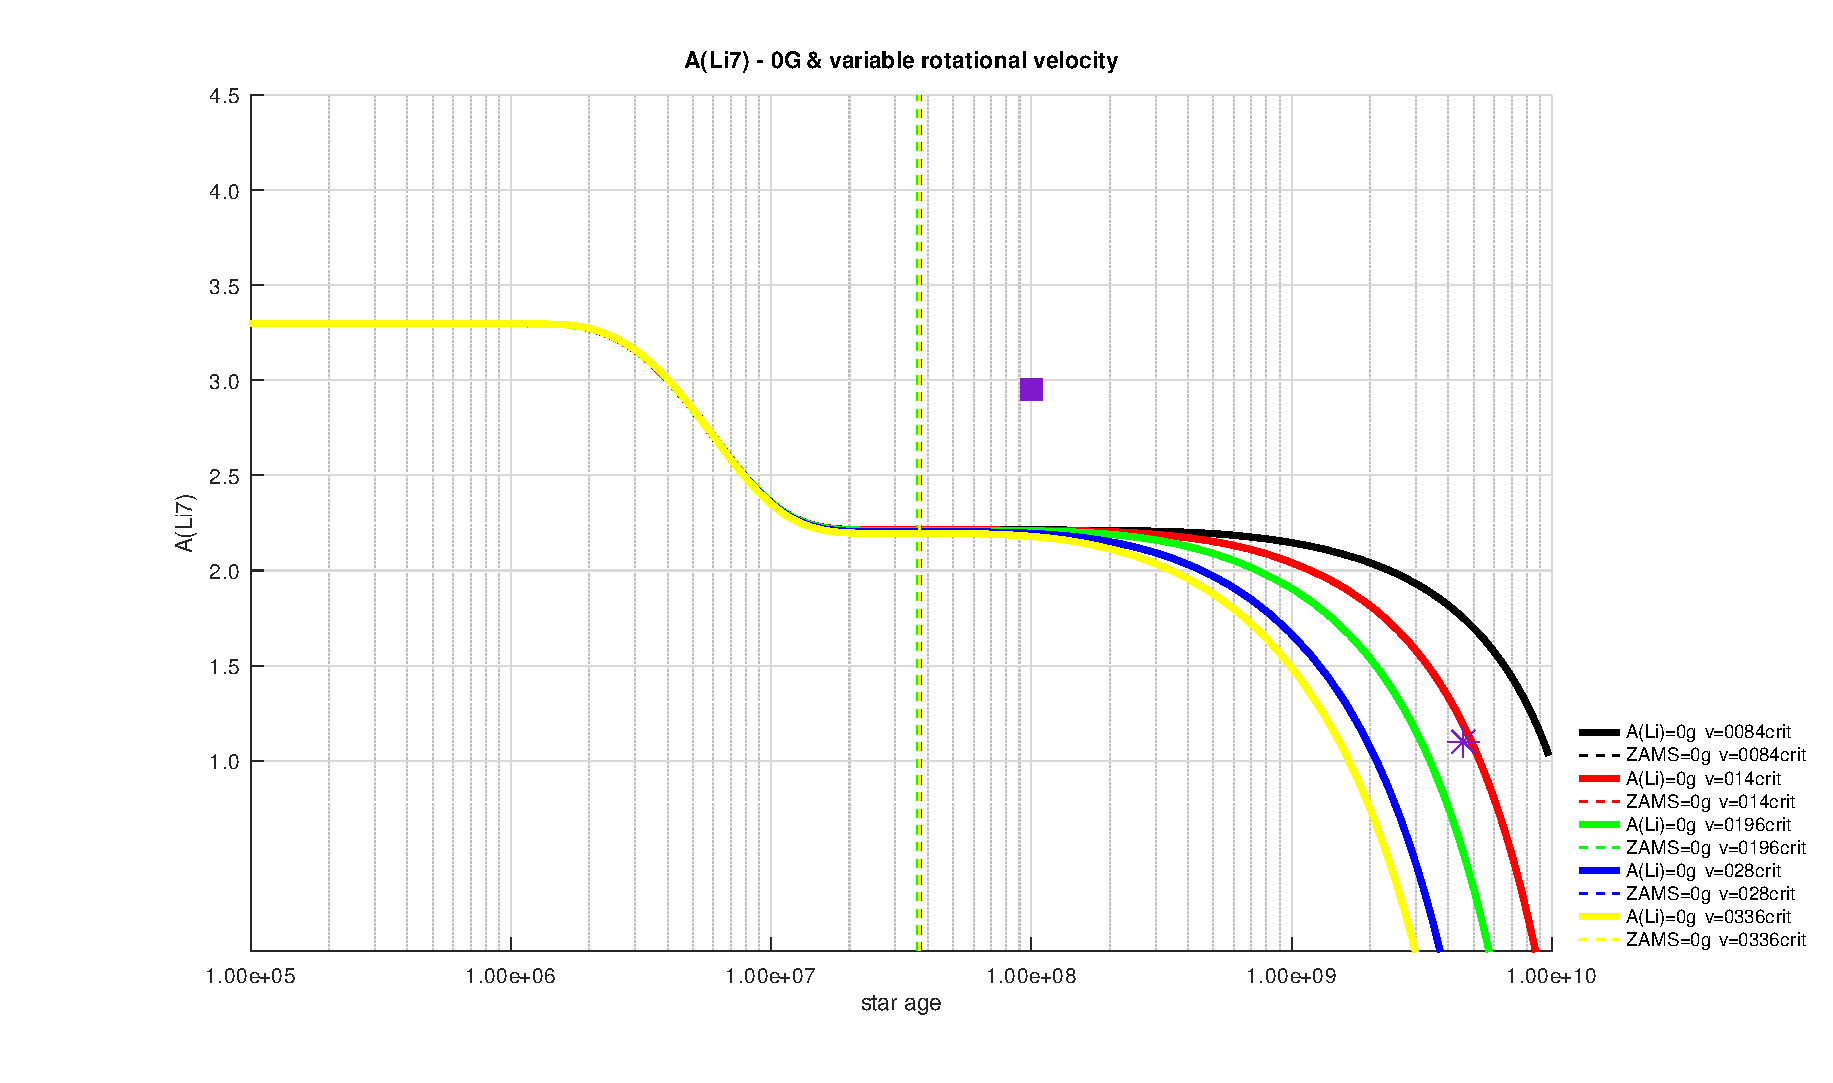
\includegraphics[width=\columnwidth]{figures/li_var_vel_0_0g.eps}
    \caption{The evolution of surface \isotope[7]{Li} abundance relative to \isotope[1]{H}, as a function of time for several 1 $M_{\sun}$ models. The solid black line represents the fiducial model according to \citet{Choi2016}. The rest of lines are models which include PMS rotation with $v/v_{crit}$ between 0.0084 and 0.0336, respectively. The purple star and square are surface Li abundance for the present-day Sun \citep{Asplund2009} and the Pleiades cluster \citep{Sestito2005} respectively. The dashed lines make reference to the ZAMS defined as the temporal simulation instant closest to the timestep in which both the central H mass fraction has been reduced by 0.0015 from its initial value and the model first $L_H/L_{phot} \geq 0.99$, where $L_{H}$ is luminosity produced by the H burning power at the star core and $L_{phot}$ represents the star luminosity in the photosphere.}
    \label{fig:li_var_vel_0g}
\end{figure}

As previously mentioned, standard stellar evolution models so far have not been able to successfully reproduce the solar surface Li abundance, indicating the need to include extra physical mechanisms. One way to account for missing physics in the models is to incorporate the effects of rotation, mixing processes and the magnetic braking. In Figure \ref{fig:li_var_vel_0g} we show the evolution of surface Li abundance relative to H as a function of time for several $1M_{\odot}$ models which take into account the effects of rotation and AML caused by stellar winds and. The purple star and square are surface Li abundance for the present-day Sun \citet{Asplund2009} and Pleiades surface Li abundance \citep{Sestito2005}.\par

In the figure (\ref{fig:li_var_vel_0g}) it can be clearly appreciated how the surface Li abundance decreases over time in all the simulated models due to the inclusion of diffusion. The solid black line represents the fiducial model that adopts the solar-calibrated envelope overshoot parameters as documented in \citet{Choi2016}. In general, all models burn too much Li early on and do not match with the Pleiades surface Li abundance. Later, the fidicual model (black line) does not deplete lithium efficiently on the MS and fail (again) to match the current solar surface Li abundance. On the other hand, the other models which include rotation during the PMS with values of $v/v_{crit}$ between 0.0084 and 0.0336 are able to burn Li in a more realistic way although only one of them (green line) is close to match the present-day Li abundance of the Sun but it rotational velocity is much higher (see fig. \ref{fig:rot_vel_0g}) than the $2 kms^{-1}$ of the Sun \citep{Gill2012} \par

Figure (\ref{fig:rot_vel_0g}) shows the photosphere rotation profile at different ages for the different rotating models. At the beginning of the PMS phase, the star is fully convective and rotates as a solid body. As soon as the radiative core develops, differential rotation takes place in the radiative zone mainly as a result of the star contracting. This effects can be clearly recognized in the figure (\ref{fig:rot_vel_cz_0g}) which shows, in addition to the angular velocity of the star surface, the velocity corresponding to the upper and lower limits of the convective zone. Differential rotation in radiative zone is directly influenced by the initial angular velocity and leads to a steep rotation profile at the base of the convective zone; the higher the initial velocity, the bigger the velocity gradient between the bottom and top limits of the convective zone. As a consequence, the turbulence strength located at the bottom of the convective envelope also increases so that the resulting mixing can transport Li to deeper and hotter regions, where it is finally destroyed in a more efficient way (see figure (\ref{fig:li_var_vel_0g})).On the other hand, the quantitative impact of rotation on the PMS Li abundance of solar-type stars seems not to be very sensitive to the initial angular velocity until the radiative core develops.\par

\begin{figure}
	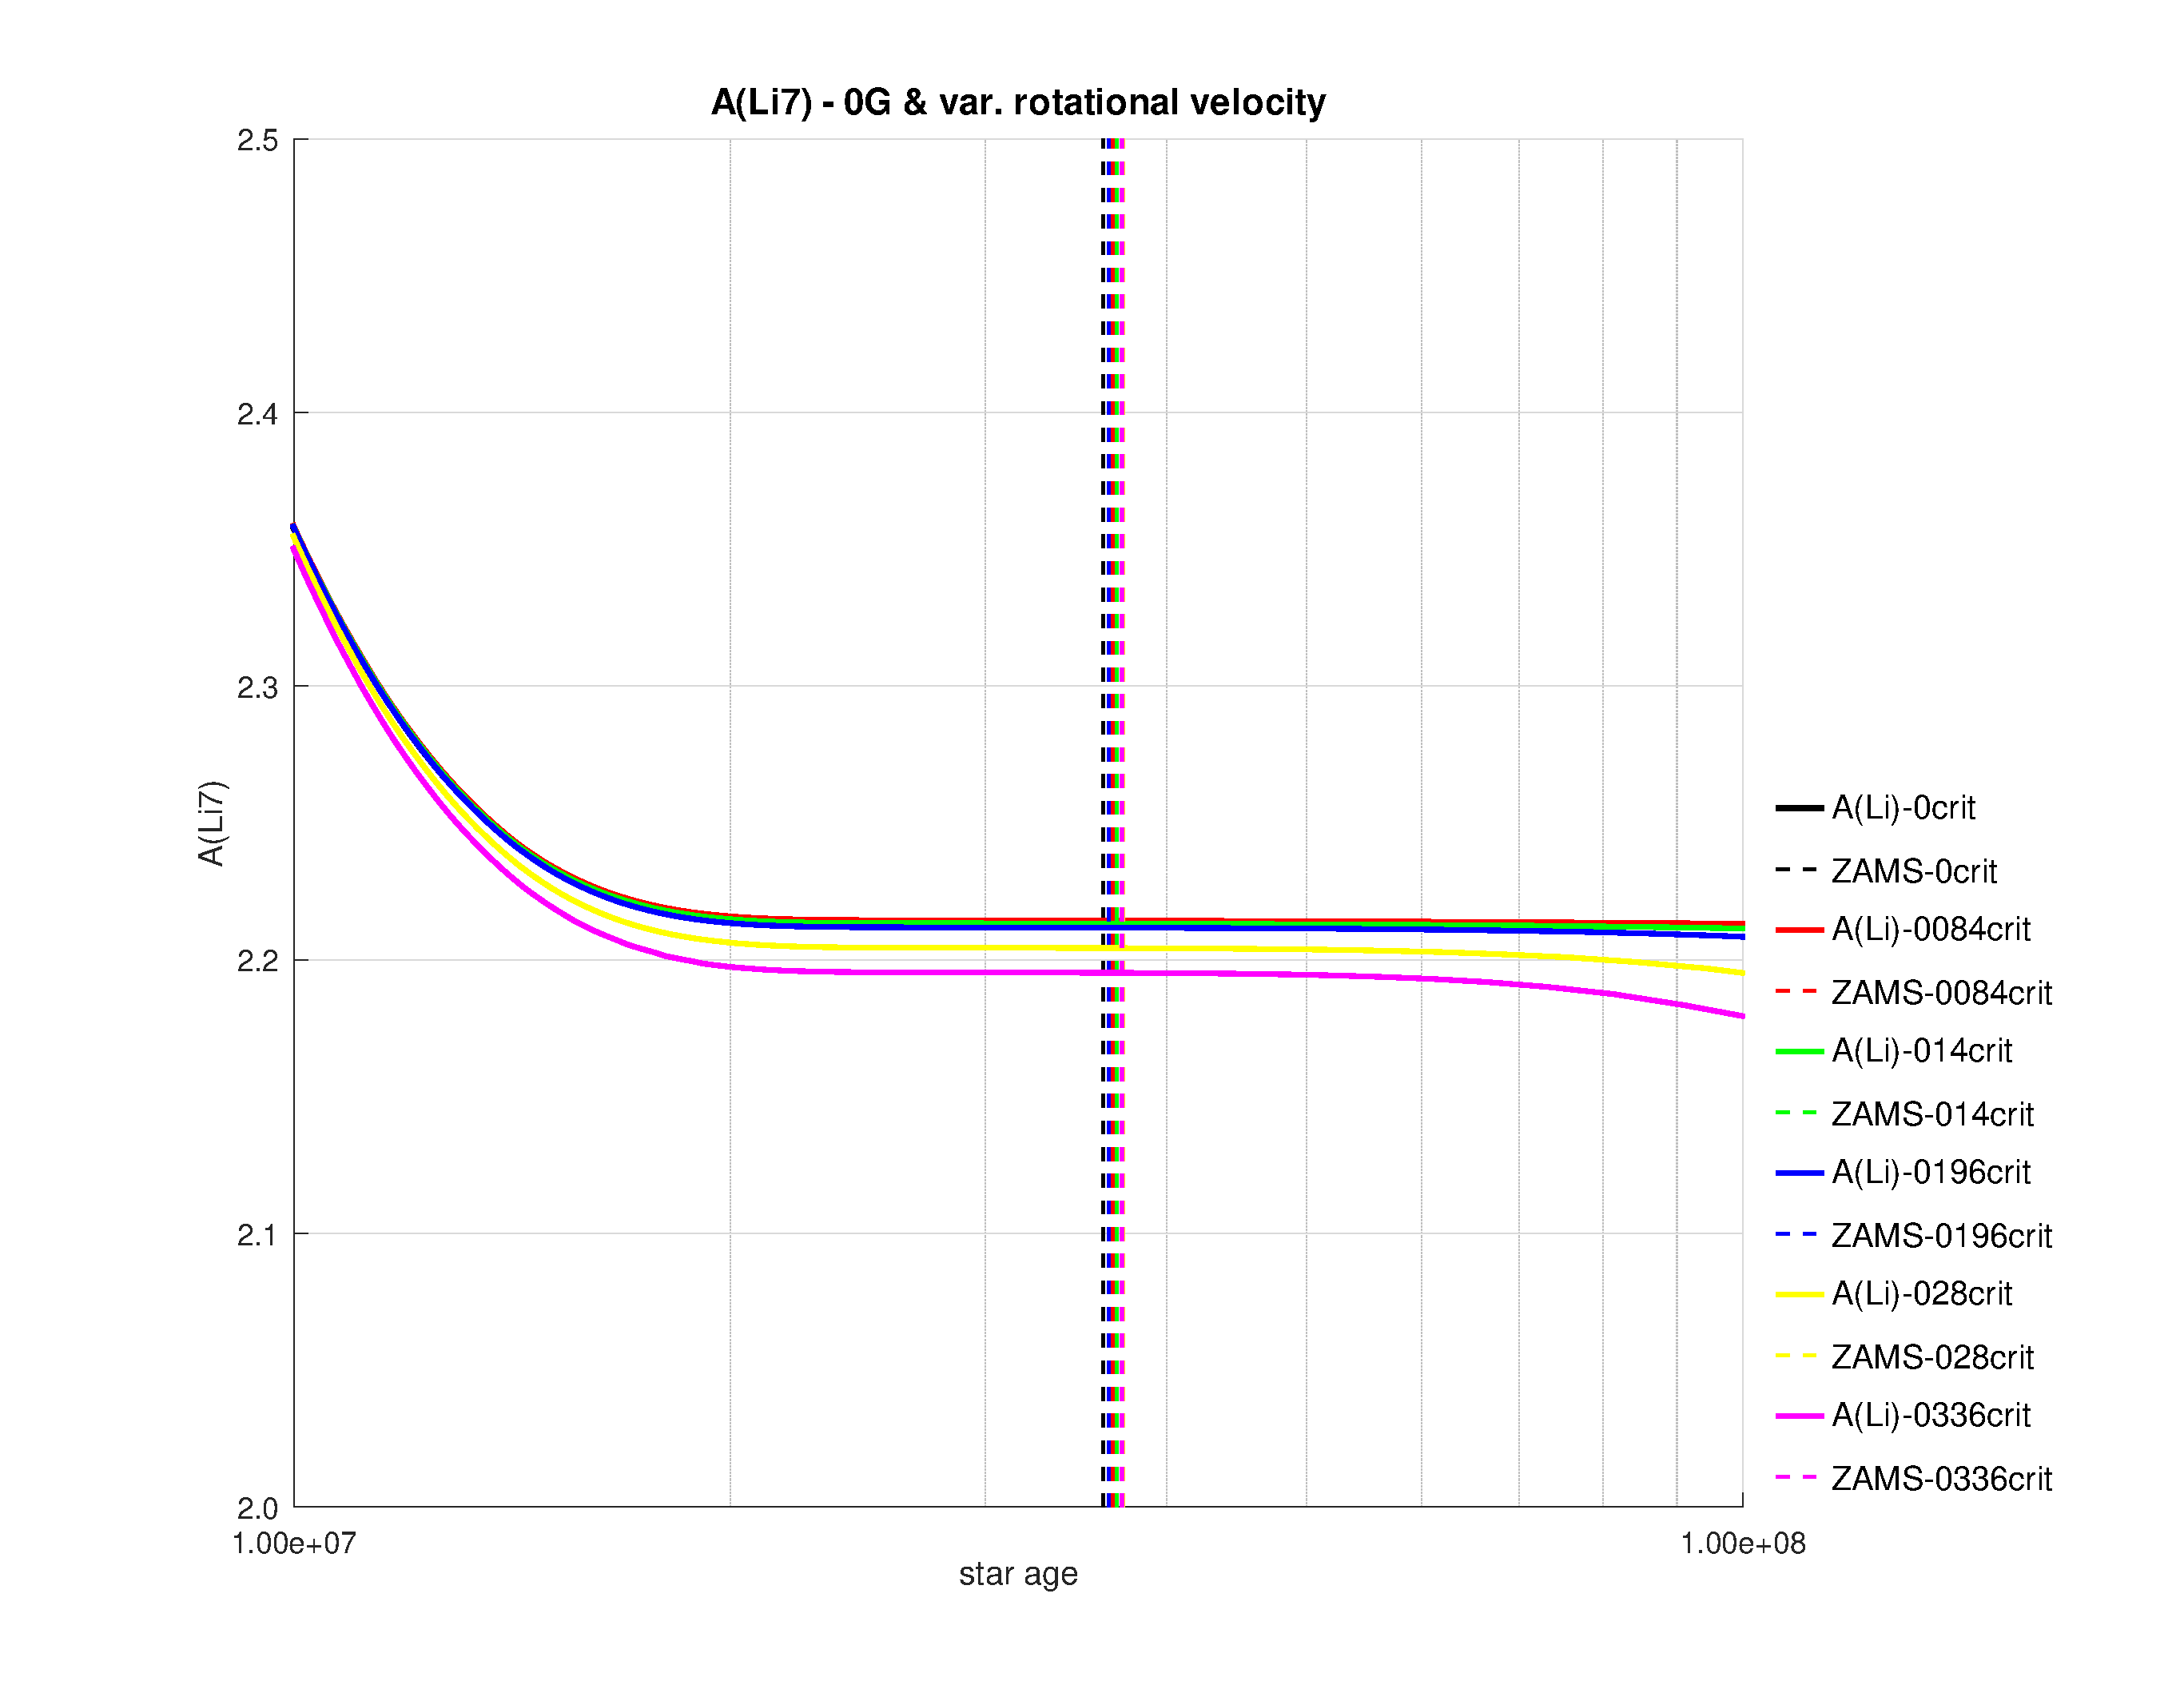
\includegraphics[width=\columnwidth]{figures/li_var_vel_0_0g_z1.eps}
    \caption {The evolution of surface \isotope[7]{Li} abundance relative to \isotope[1]{H}, as a function of time for several 1 $M_{\sun}$ models in the approach to the ZAMS (dashed lines). The solid black line represents the fiducial model according to \citet{Choi2016}. The rest of lines are models with includes PMS rotation with $v/v_{crit}$ between 0.0084 and 0.0336, respectively.}
    \label{fig:li_var_vel_0g_z1}
\end{figure}


The evolutionary tracks in the HR diagram are shown for the models in figure (\ref{fig:hr_var_vel_0g}). A well known structural effect of rotation is the decrease of the effective temperature and to a less extent of stellar luminosity. These results are in line with those of previous studies (see e.g. \citet{Eggenberger2012}, \citet{Piau2001}, \citet{Pinsonneault1989}). Figure (\ref{fig:li_var_vel_0g_z1}) shows a zoomed-in view of evolution tracks from the ZAMS till the TAMS in which the aforementioned effects caused by rotation are easily recognized. As depicted in figure (\ref{fig:li_var_vel_0g_z1}) at the end of the PMS, the rotating models exhibits a lower surface Li abundance than the non-rotating one. We thus see that the inclusion of rotation results in a global increase of the Li depletion during the PMS. We also note that the Li depletion occurs earlier for the rotating model than for the non-rotating.\par


\begin{figure}
	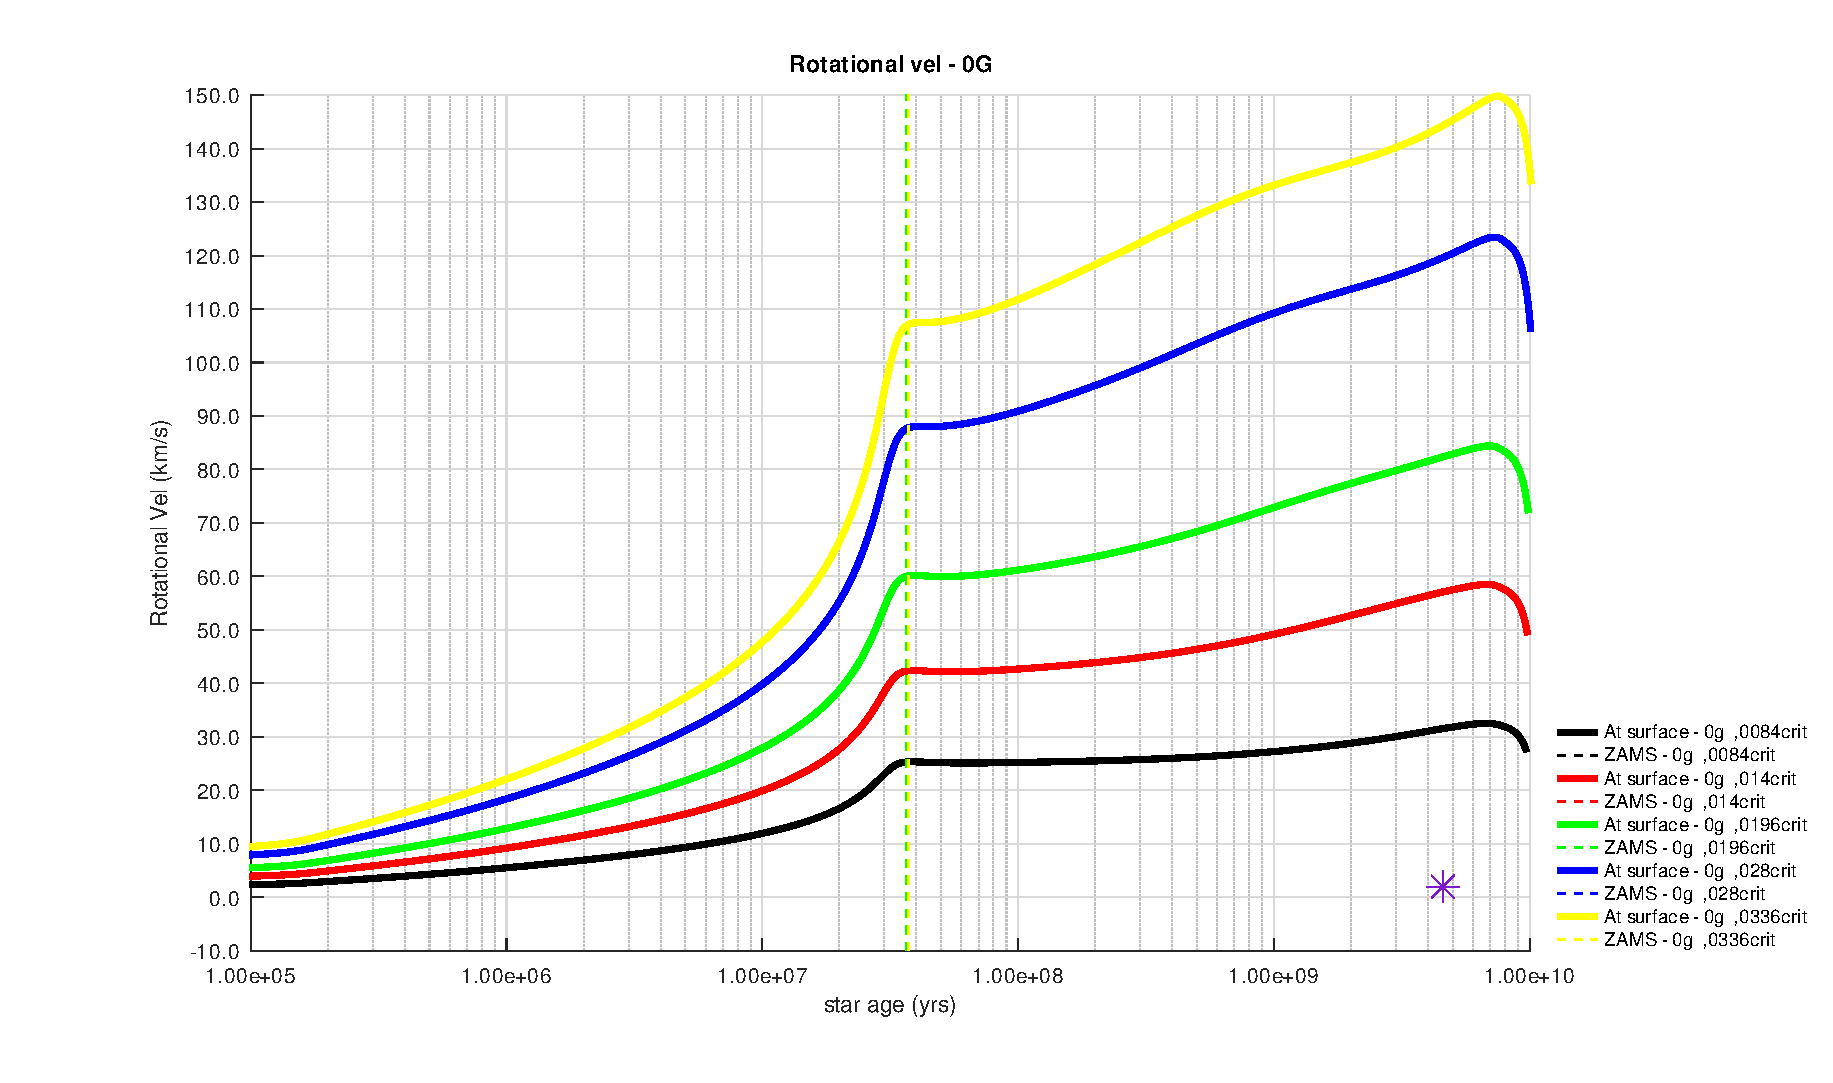
\includegraphics[width=\columnwidth]{figures/rot_vel_0g.eps}
    \caption{The evolution of surface rotational velocity, as a function of time for several 1 $M_{\sun}$ models. The lines are models with includes PMS rotation with $v/v_{crit}$ between 0.0084 and 0.0336, respectively. The purple star is the surface angular velocity for the present-day Sun \citep{Gill2012}. The dashed lines make reference to the ZAMS.}
    \label{fig:rot_vel_0g}
\end{figure}

\begin{figure}
	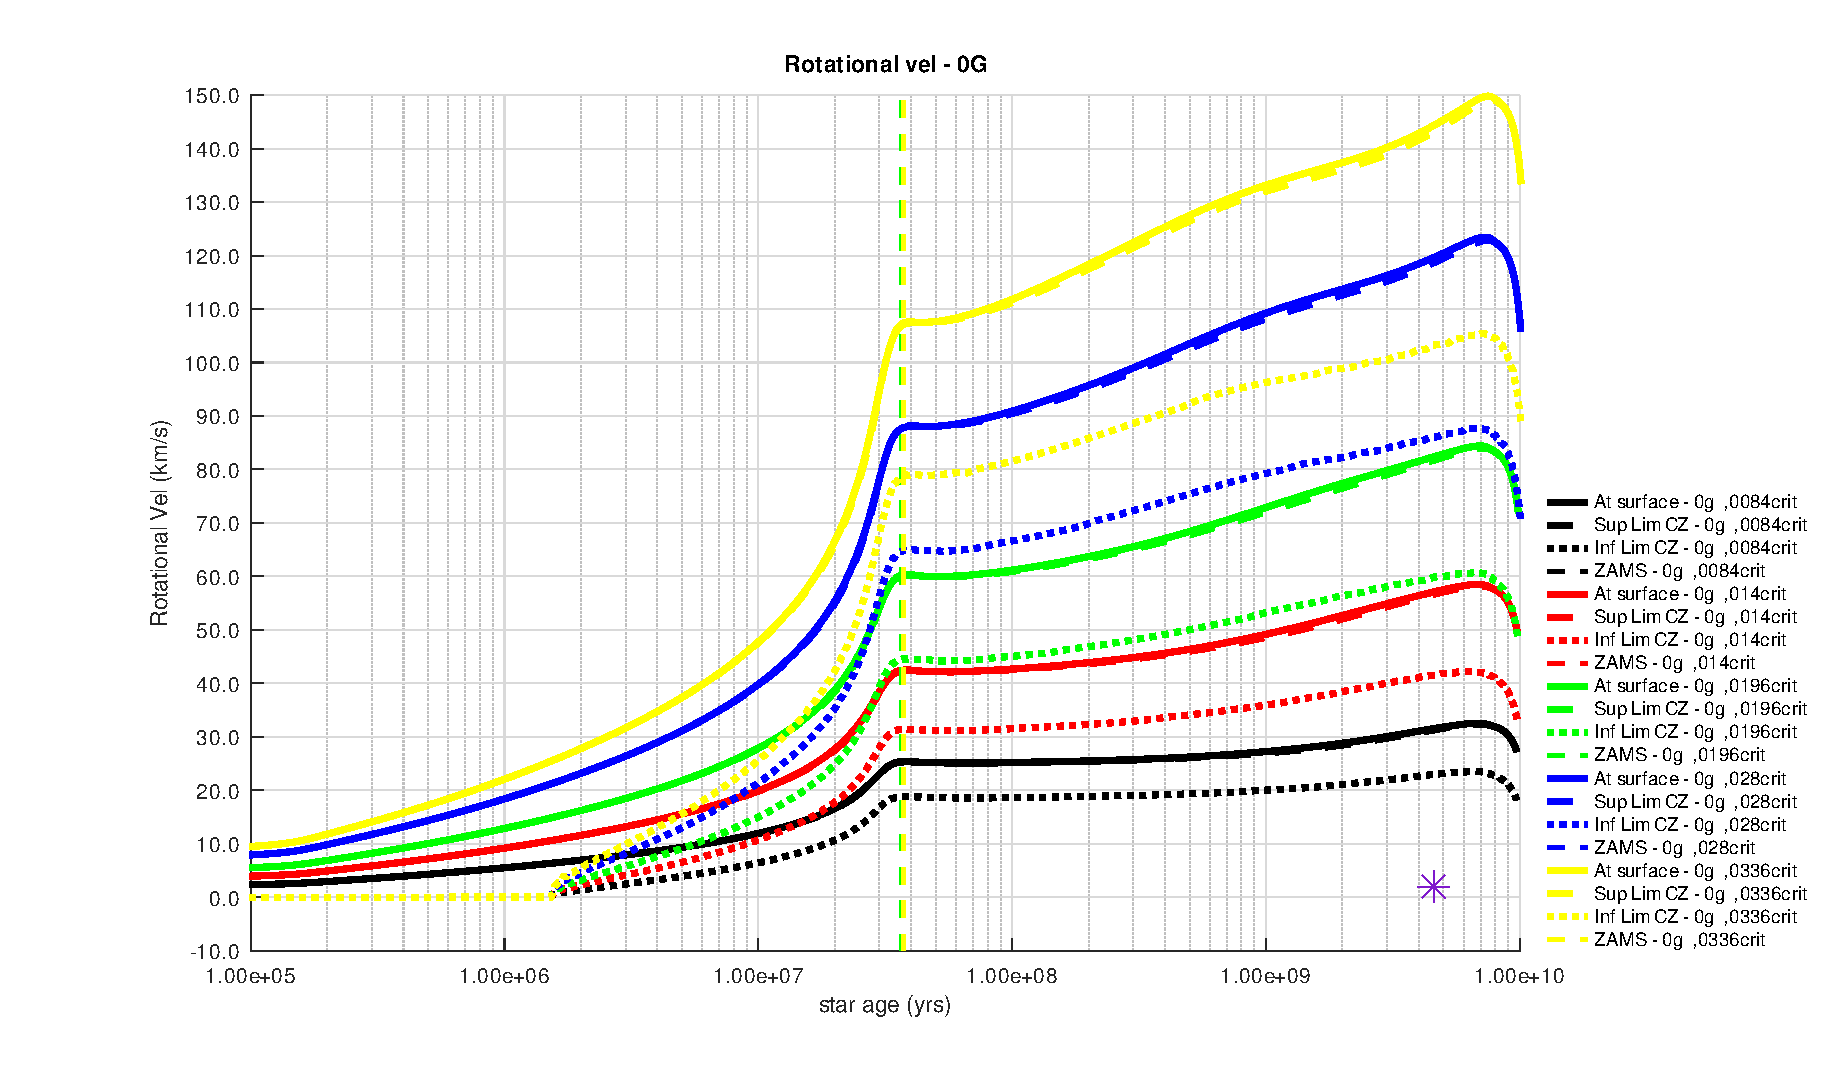
\includegraphics[width=\columnwidth]{figures/rot_vel_cz_0g.eps}
    \caption{The evolution of angular velocity at surface and limits of the uppermost convective zone, as a function of time for several 1 $M_{\sun}$ models. The lines are models with includes PMS rotation with $v/v_{crit}$ between 0.0084 and 0.0336, respectively. The purple star is the surface angular velocity for the present-day Sun \citep{Gill2012}. The dashed lines make reference to the ZAMS.}
    \label{fig:rot_vel_cz_0g}
\end{figure}

\begin{figure}
	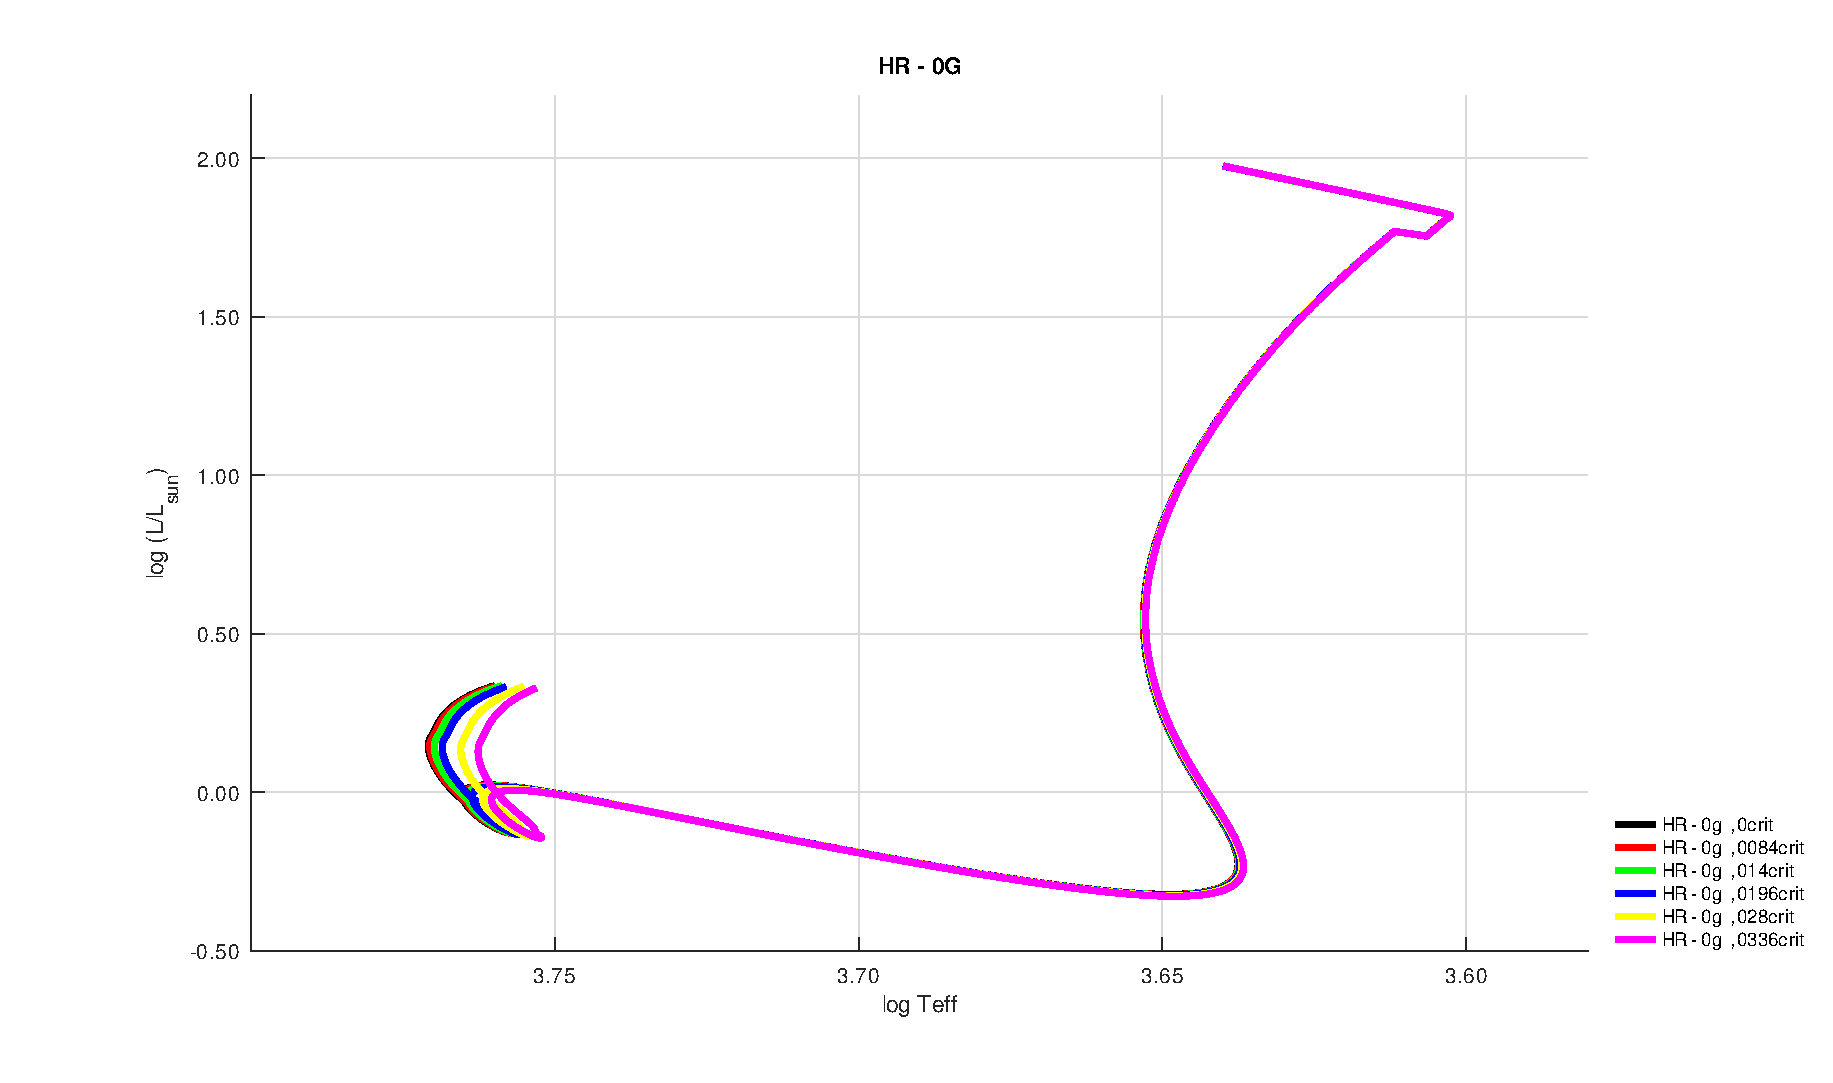
\includegraphics[width=\columnwidth]{figures/hr_var_vel_0g.eps}
    \caption{An example solar 1$M_{\sun}$ grid of stellar evolutionary track from PMS till TAMS covering a wide range of angular velocities. The rotation is activated in the models in the PMS.}
    \label{fig:hr_var_vel_0g}
\end{figure}

\begin{figure}
	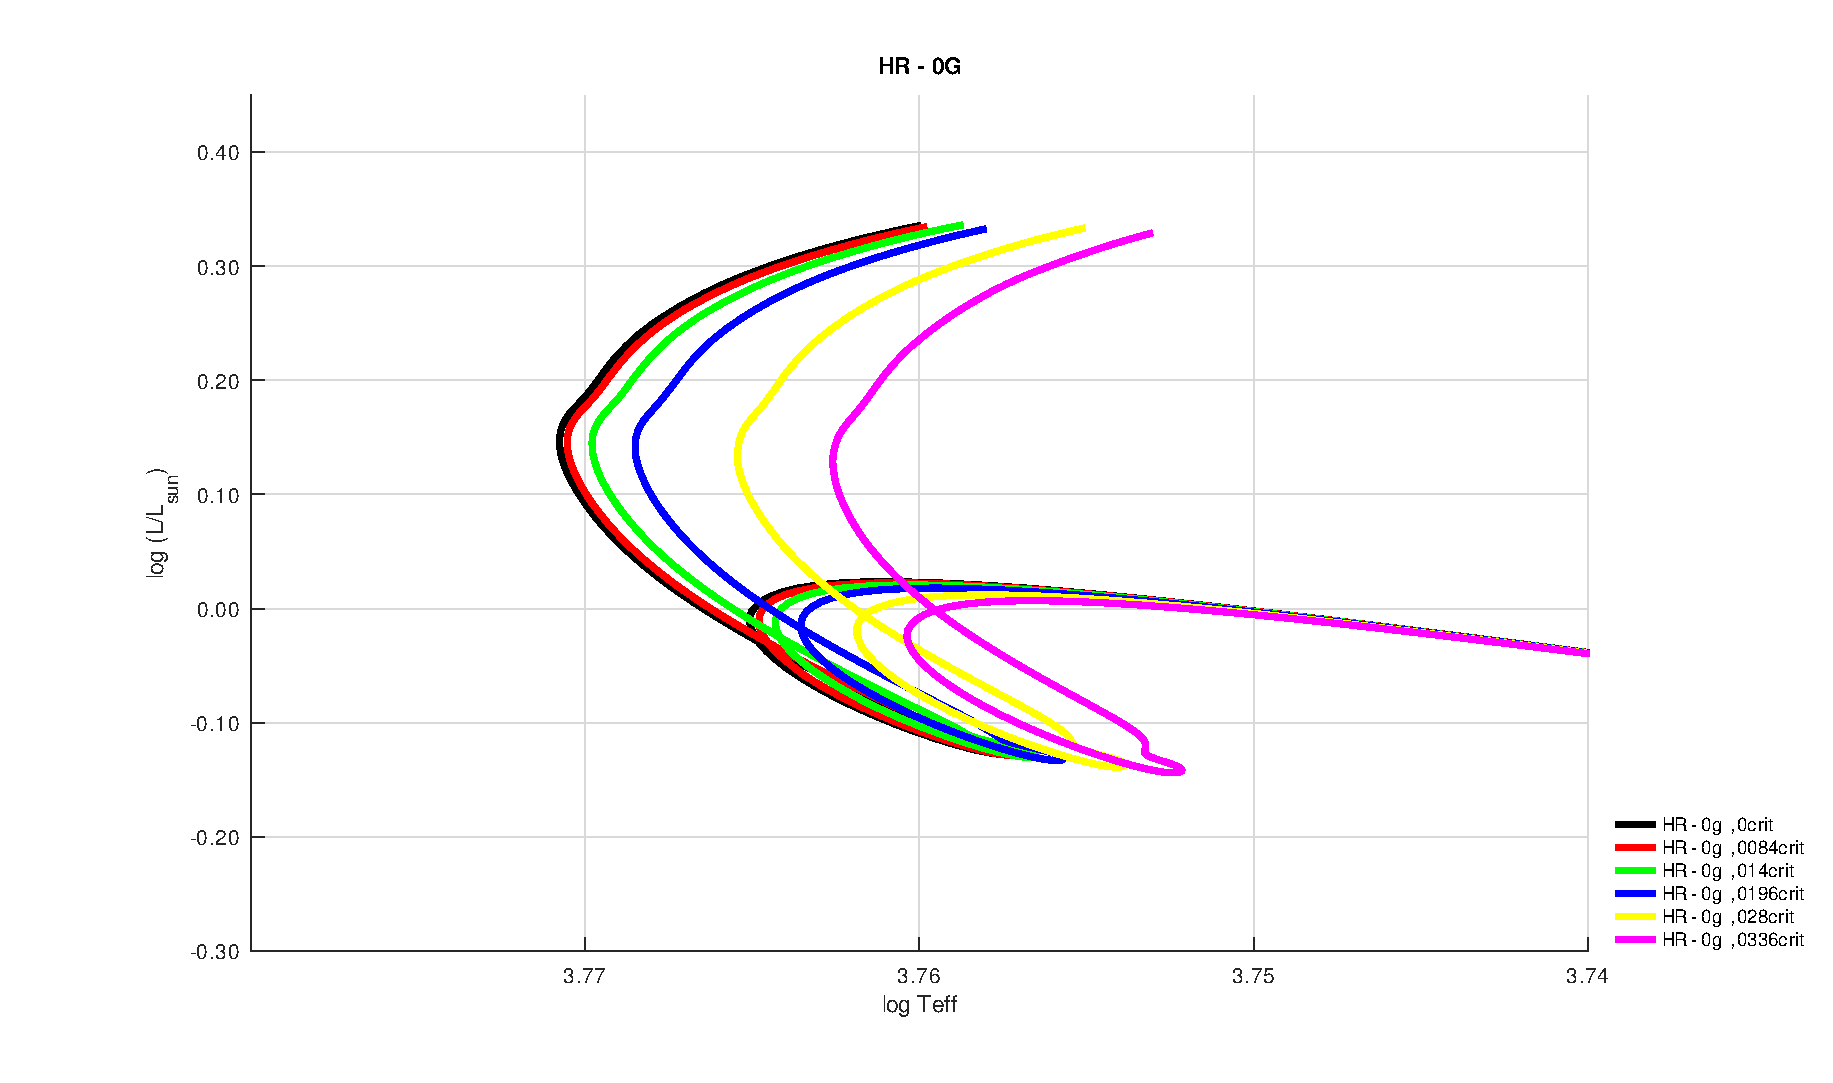
\includegraphics[width=\columnwidth]{figures/hr_var_vel_0g_z1.eps}
    \caption{Similar to figure (\ref{fig:hr_var_vel_0g}) but now showing in detail the effects of rotation on the evolutionary tracks.}
    \label{fig:hr_var_vel_0g_z1}
\end{figure}


\subsection{Magnetic braking and Li evolution}
In the rest of this document we are going to focus, unless otherwise indicated, on models that include rotation from the PMS since they are the ones that can offer a greater approximation to the observations. In turn, these models will serve as a basis for others in which our magnetic braking routine is used by simulating magnetic fields of different intensity, varying from 3.5G to 5.5G in 0.5G increments.\par

If we concentrate our attention on figure (\ref{fig:li_var_vel_4_0g}) and compare it with figure (\ref{fig:li_var_vel_0g}) we will see how the profiles of Li abundance are already altered during PMS and MS. In the first phase we can describe the effect as modest, somewhat expected and in line with the fact that the loss of angular momentum caused by magnetic braking (see equation (\ref{eq:j_dot})) depends directly on the loss of mass. If we take into account that for solar type stars the models predict a modest total loss of mass, this is even much lower during PMS. On the contrary, during the MS it is observed in a much more evident way how the loss of angular momentum is much more significant, causing the star to rotate more slowly and as a result a smaller amount of Li to be destroyed.\par

\begin{figure}
	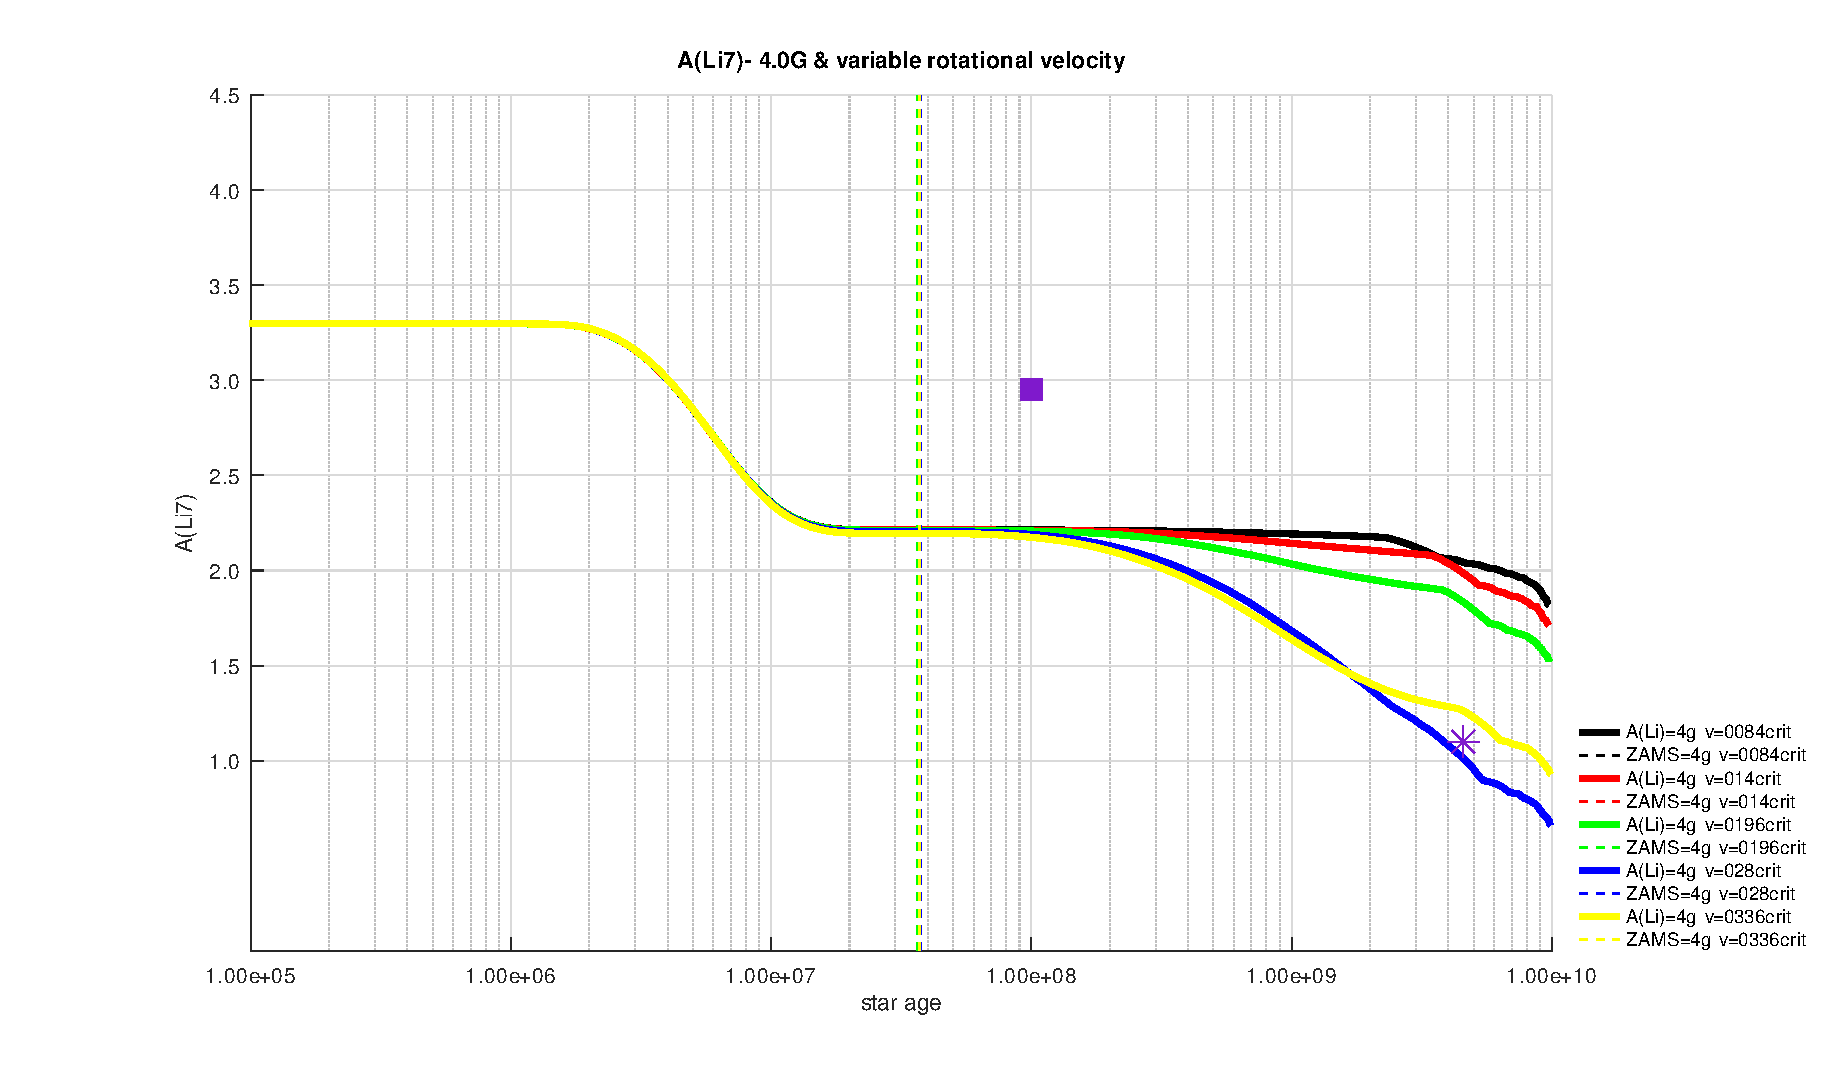
\includegraphics[width=\columnwidth]{figures/li_var_vel_4_0g.eps}
    \caption{The evolution of surface \isotope[7]{Li} abundance relative to \isotope[1]{H}, as a function of time for several 1 $M_{\sun}$ models. The models include a magnetic field with an intensity of 4G and PMS rotation with $v/v_{crit}$ between 0.0084 and 0.0336, respectively. The purple star and square are surface Li abundance for the present-day Sun \citep{Asplund2009} and the Pleiades cluster \citep{Sestito2005} respectively. The dashed lines make reference to the ZAMS.}
    \label{fig:li_var_vel_4_0g}
\end{figure}

The effect of the magnetic braking routine can be seen even more clearly in figure (\ref{fig:rot_vel_4g}). Here we represent the rotation profiles on the surface of the stars for different rotating models. As it can be observed, and in a similar way to the evolution profiles of the Li on the surface commented in the previous paragraph, the effect of the routine is much more accentuated once the ZAMS is reached. If the evolution of the curves presented here with those of figure (\ref{fig:rot_vel_0g}) we see how the star, instead of continuing to increase its angular velocity, begins to slow down after having reached its maximum in the passage through the ZAMS.\par

We also find it interesting to highlight the behaviour of angular velocity profiles when approaching TAMS. As can be seen in figure (\ref{fig:rot_vel_4g}) and in more detail in (\ref{fig:rot_vel_4g_z1}), we find that the evolution of angular velocity suffers from a series of ups and downs that do not appear previously. Everything seems to indicate that this behavior is due to a combined effect of the magnetic braking routine and the time-step (probably to big) used by MESA during the last part of the simulation. We based this affirmation on the fact that this effect is not observed in the series of simulations in which the routine is not included (figs. (\ref{fig:rot_vel_0g}) and (\ref{fig:rot_vel_cz_0g})).\par

\begin{figure}
	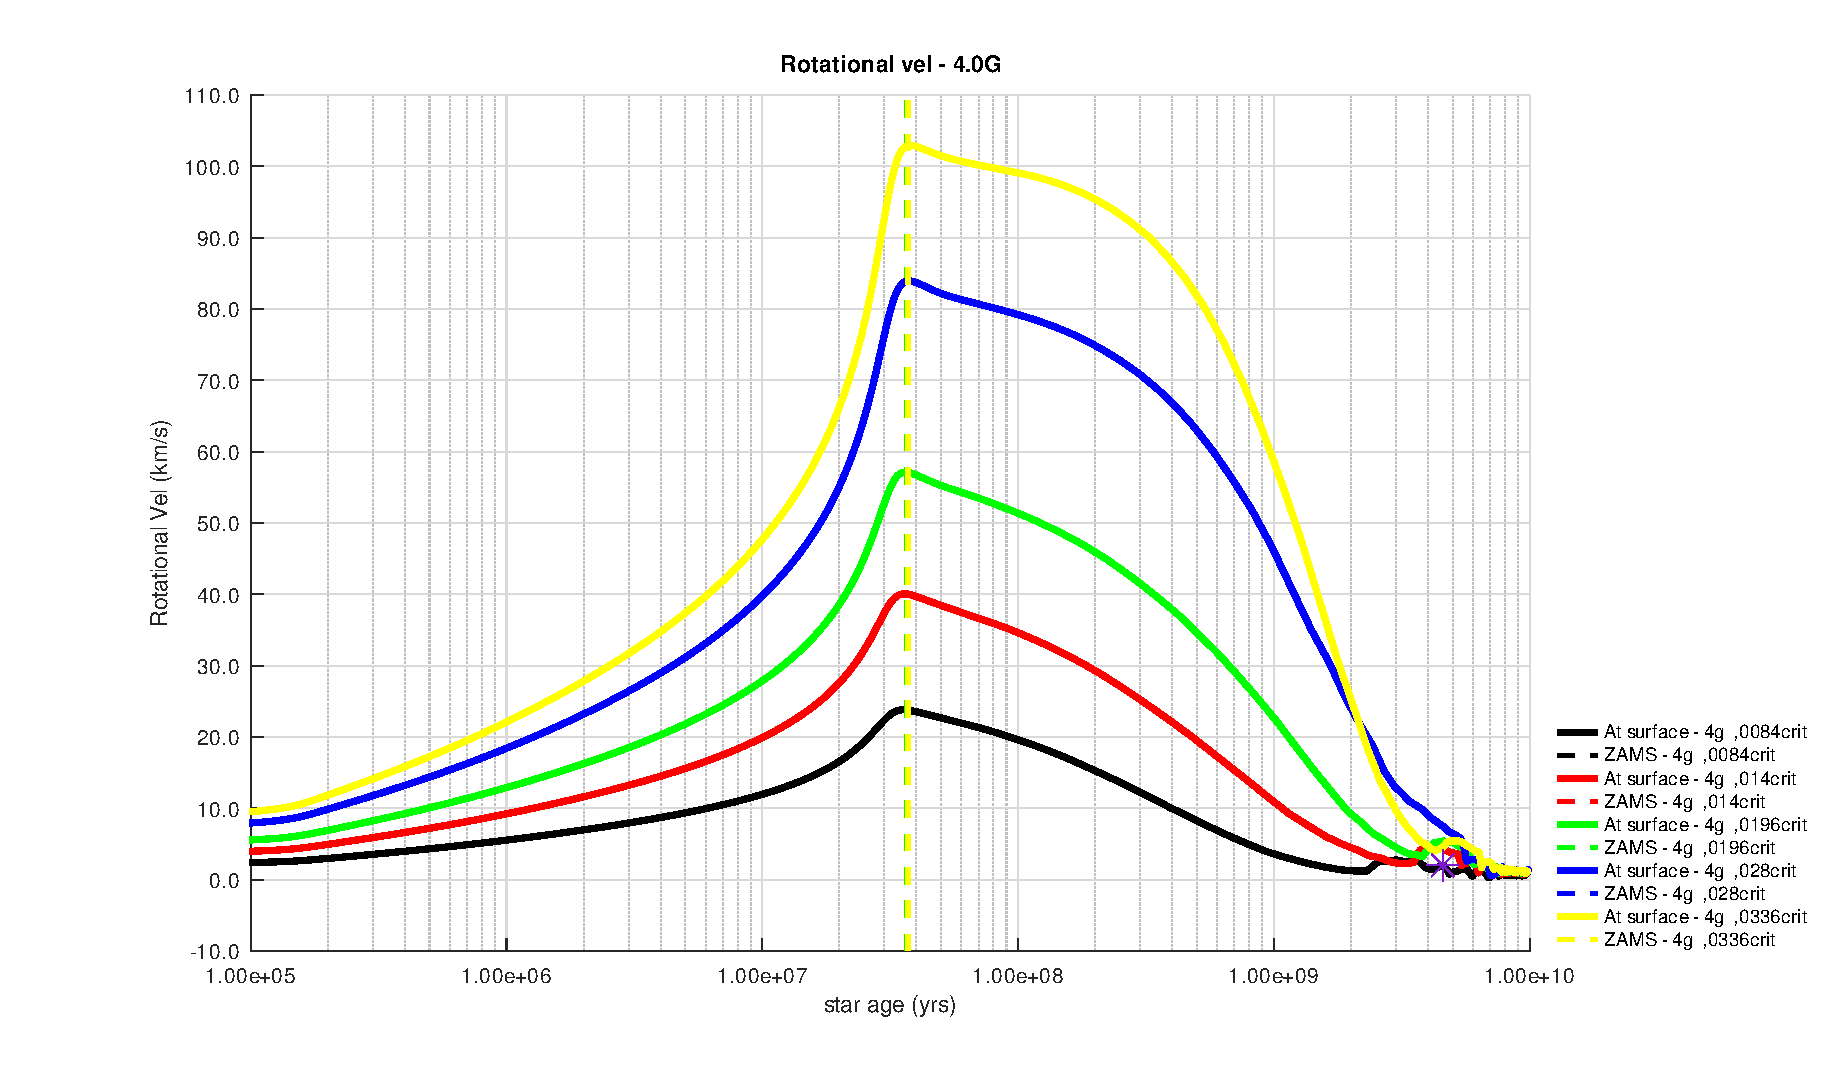
\includegraphics[width=\columnwidth]{figures/rot_vel_4g.eps}
    \caption{The evolution of surface rotational velocity, as a function of time for several 1 $M_{\sun}$ models. The models include a magnetic field with an intensity of 4G and PMS rotation with $v/v_{crit}$ between 0.0084 and 0.0336, respectively. Additionally it's simulated the magnetic braking effect of magnetic field with an intensity of 4G. The purple star is the surface angular velocity for the present-day Sun \citep{Gill2012}. The dashed lines make reference to the ZAMS.}
    \label{fig:rot_vel_4g}
\end{figure}

\begin{figure}
	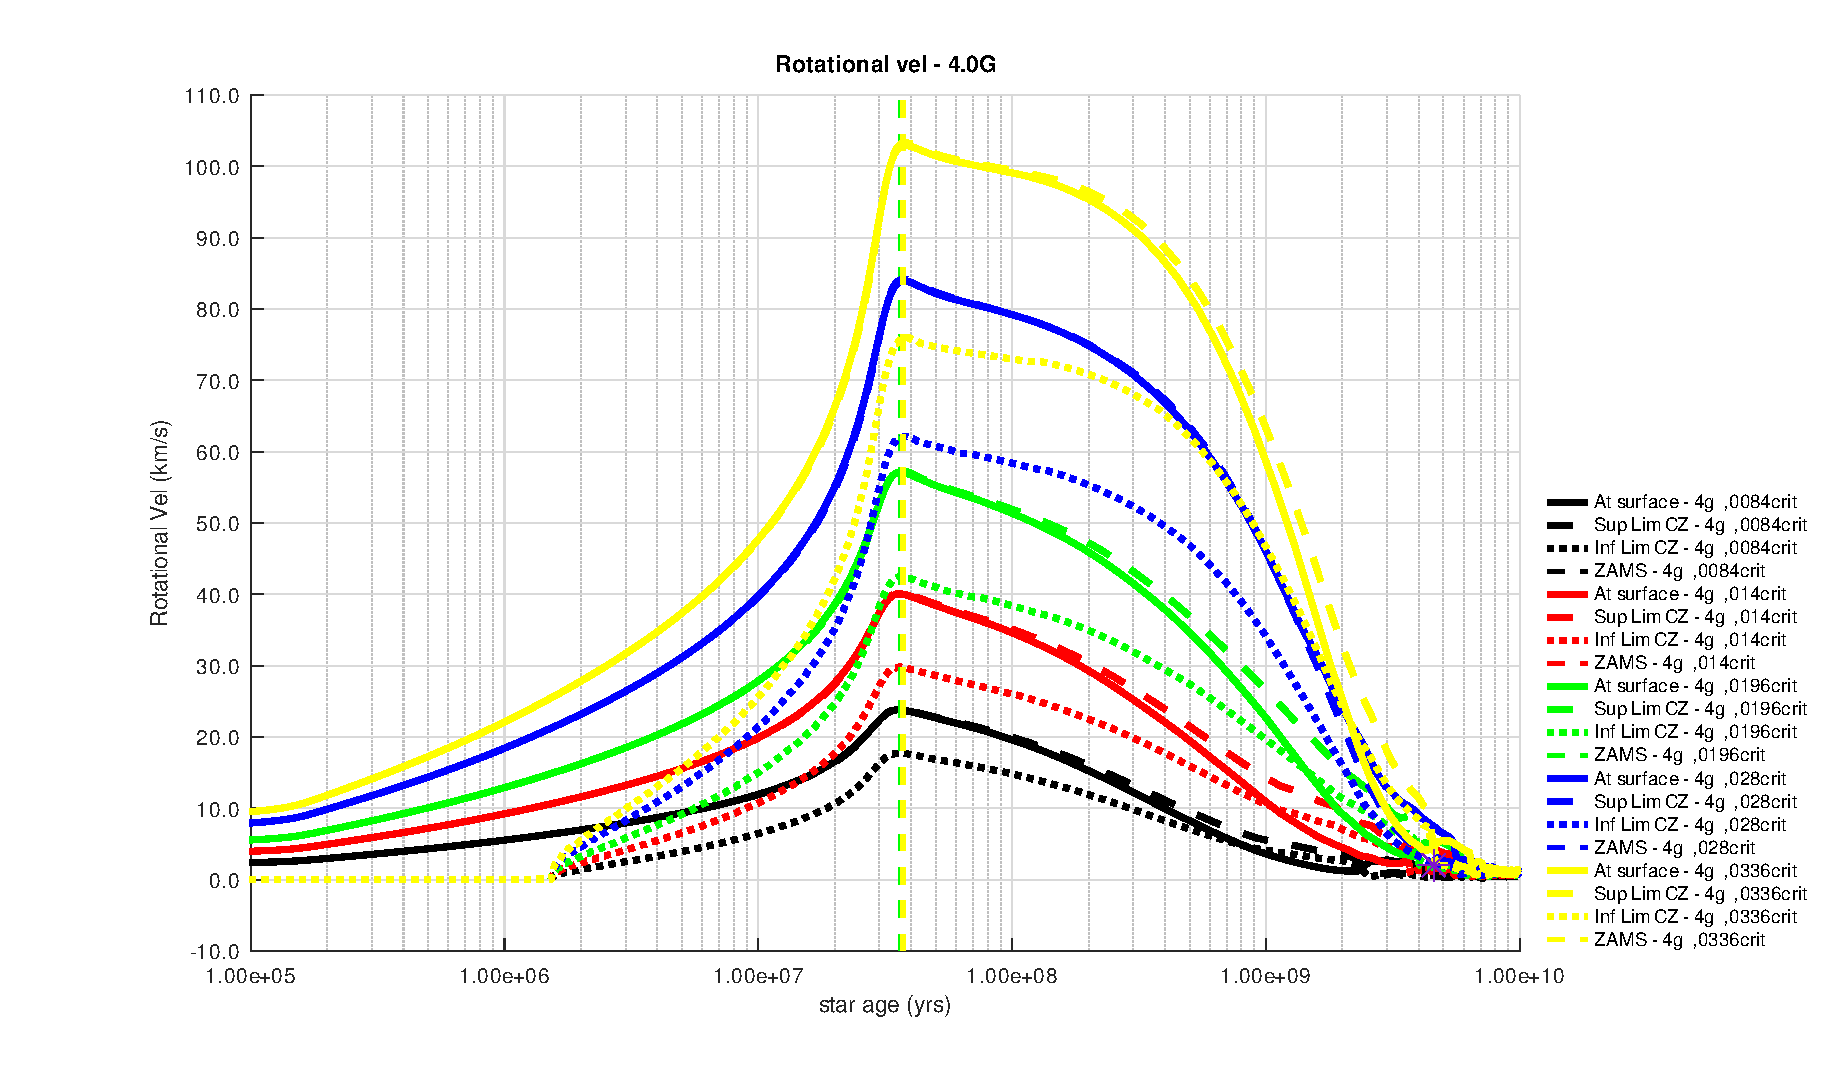
\includegraphics[width=\columnwidth]{figures/rot_vel_cz_4g.eps}
    \caption{The evolution of angular velocity at surface and limits of the uppermost convective zone, as a function of time for several 1 $M_{\sun}$ models. The lines are models with includes PMS rotation with $v/v_{crit}$ between 0.0084 and 0.0336, respectively. The dashed lines make reference to the ZAMS.}
    \label{fig:rot_vel_cz_4g}
\end{figure}

\begin{figure}
	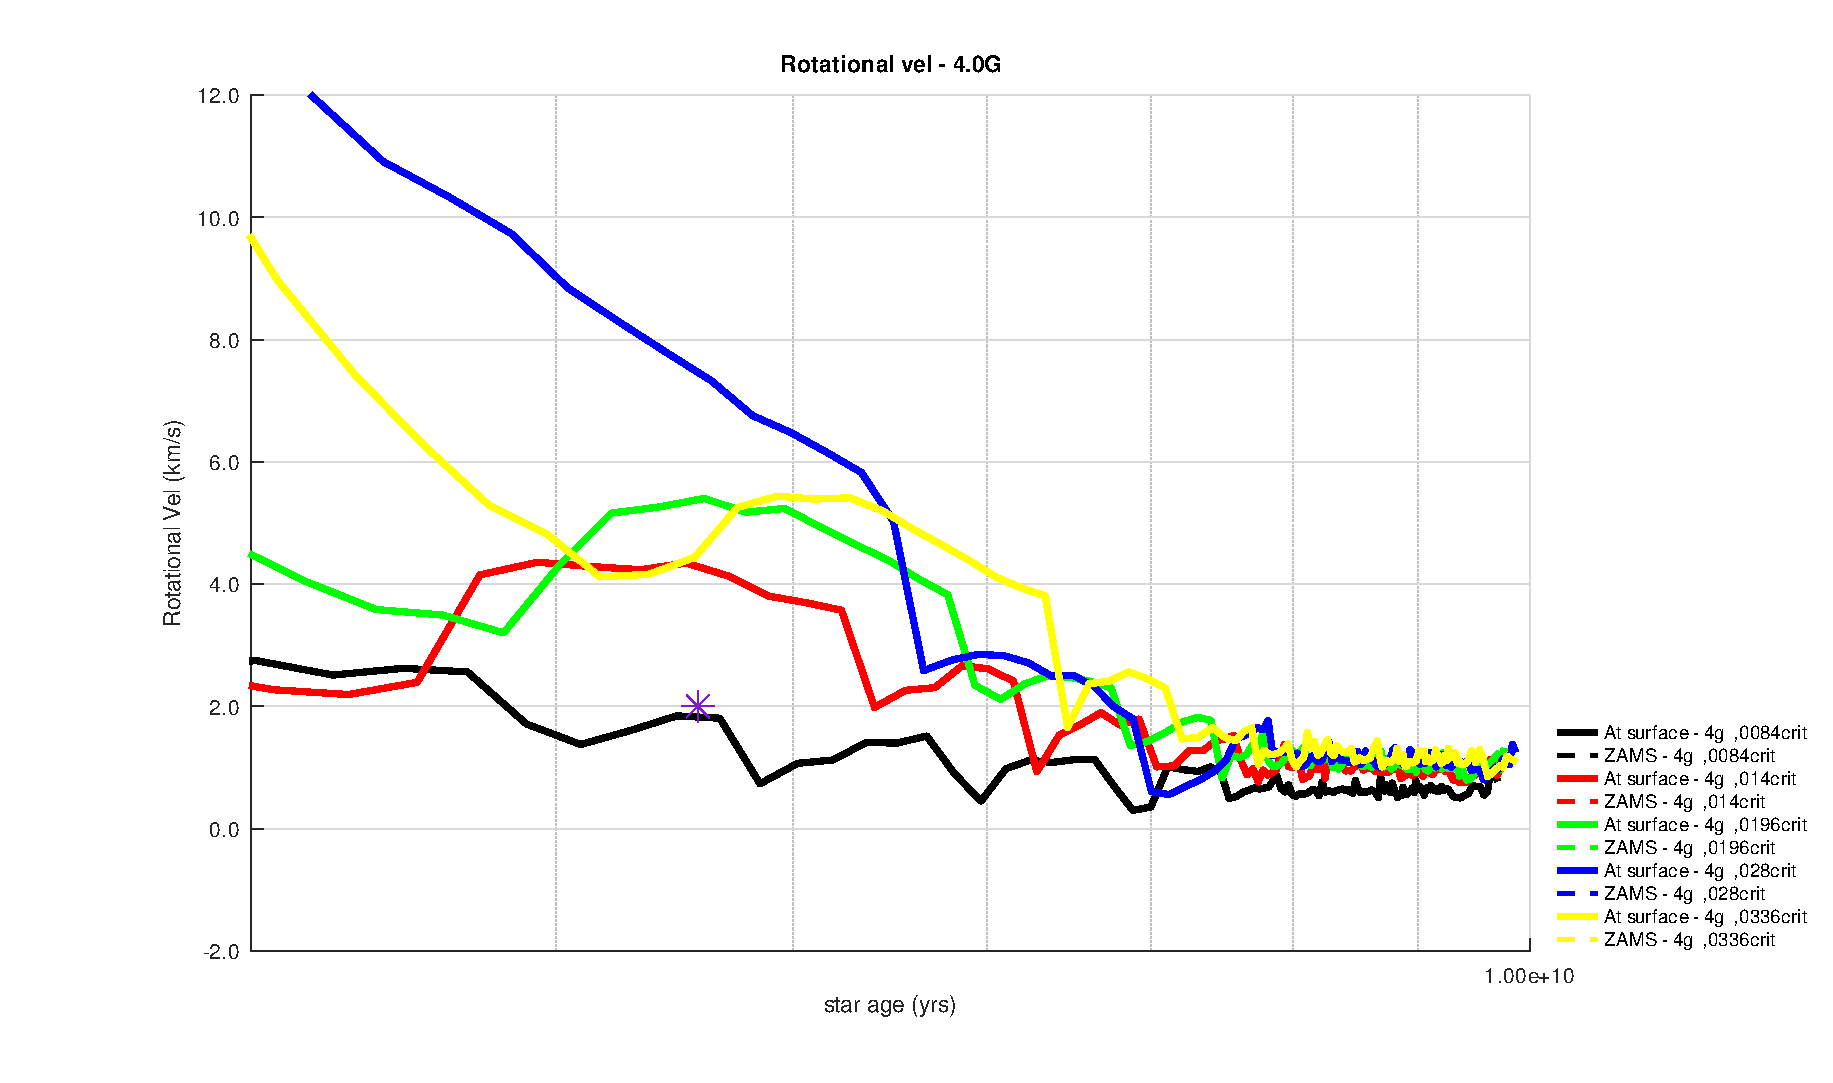
\includegraphics[width=\columnwidth]{figures/rot_vel_4g_z1.eps}
    \caption{Similar to figure (\ref{fig:rot_vel_4g}) but now showing in detail the surface rotational velocity as the star approaches TAMS.}
    \label{fig:rot_vel_4g_z1}
\end{figure}

It's also remarkable to highlight the lower angular velocity observed in figure (\ref{fig:rot_vel_cz_4g} at the star surface in comparison with the upper limit of the convective layer. This fact is most probably a consequence of the expansion of the superficial layers after the mass loss produced by stellar winds.\par


As mentioned above, the magnetic braking routine distributes the total amount of AML calculated according to equation (\ref{eq:k_jdot}) among the different layers that compose it. In figure (\ref{fig:cz_vc_028_var_b}) we can observe the evolution of the most external convective zone normalized with respect to the radius of the star. In accordance with the established models of stellar evolution, in a solar-type star the convective zone covers practically all of it for a large part of the PMS. As it approaches ZAMS it is decreasing, as a consequence of the appearance of a radiative core, maintaining an approximately constant radius until the final stage of the MS, where it increases significantly as a response to the generalized increase of the star's radius. Regarding the effect of magnetic braking on the size of the convective zone, we observe that as the intensity of the magnetic field increases, the size of the convective zone decreases. According to \citet{Jeffries2004} this direct consequence is expected because the magnetic fields in the convective zone raise the adiabatic temperature gradient and accelerate the formation of a radiative core. This radiative core pushes outward to include a rapidly increasing fraction of the stellar mass, making that the temperature at the BCZ drops below the one required for burning Li. This effect is most evident during MS (fig. (\ref{fig:cz_vc_028_var_b_z1})). The decrease in the size of the convective zone is in line with the fact that less Li is destroyed by causing less star material to reach areas with temperatures above $T_{Li}$. \par

Similar to the evolution of the angular velocity towards the end of the MS discussed in the previous paragraph, we observe that the size of the convective zone also shows a series of ups and downs. Again we think that this effect is a direct consequence of the temporal resolution used by MESA in the stellar evolution equations. The specific origin of these fluctuations is a subject that we will deal with in more depth and detail the origin of these fluctuations in subsequent works to the current one.\par

\begin{figure}
	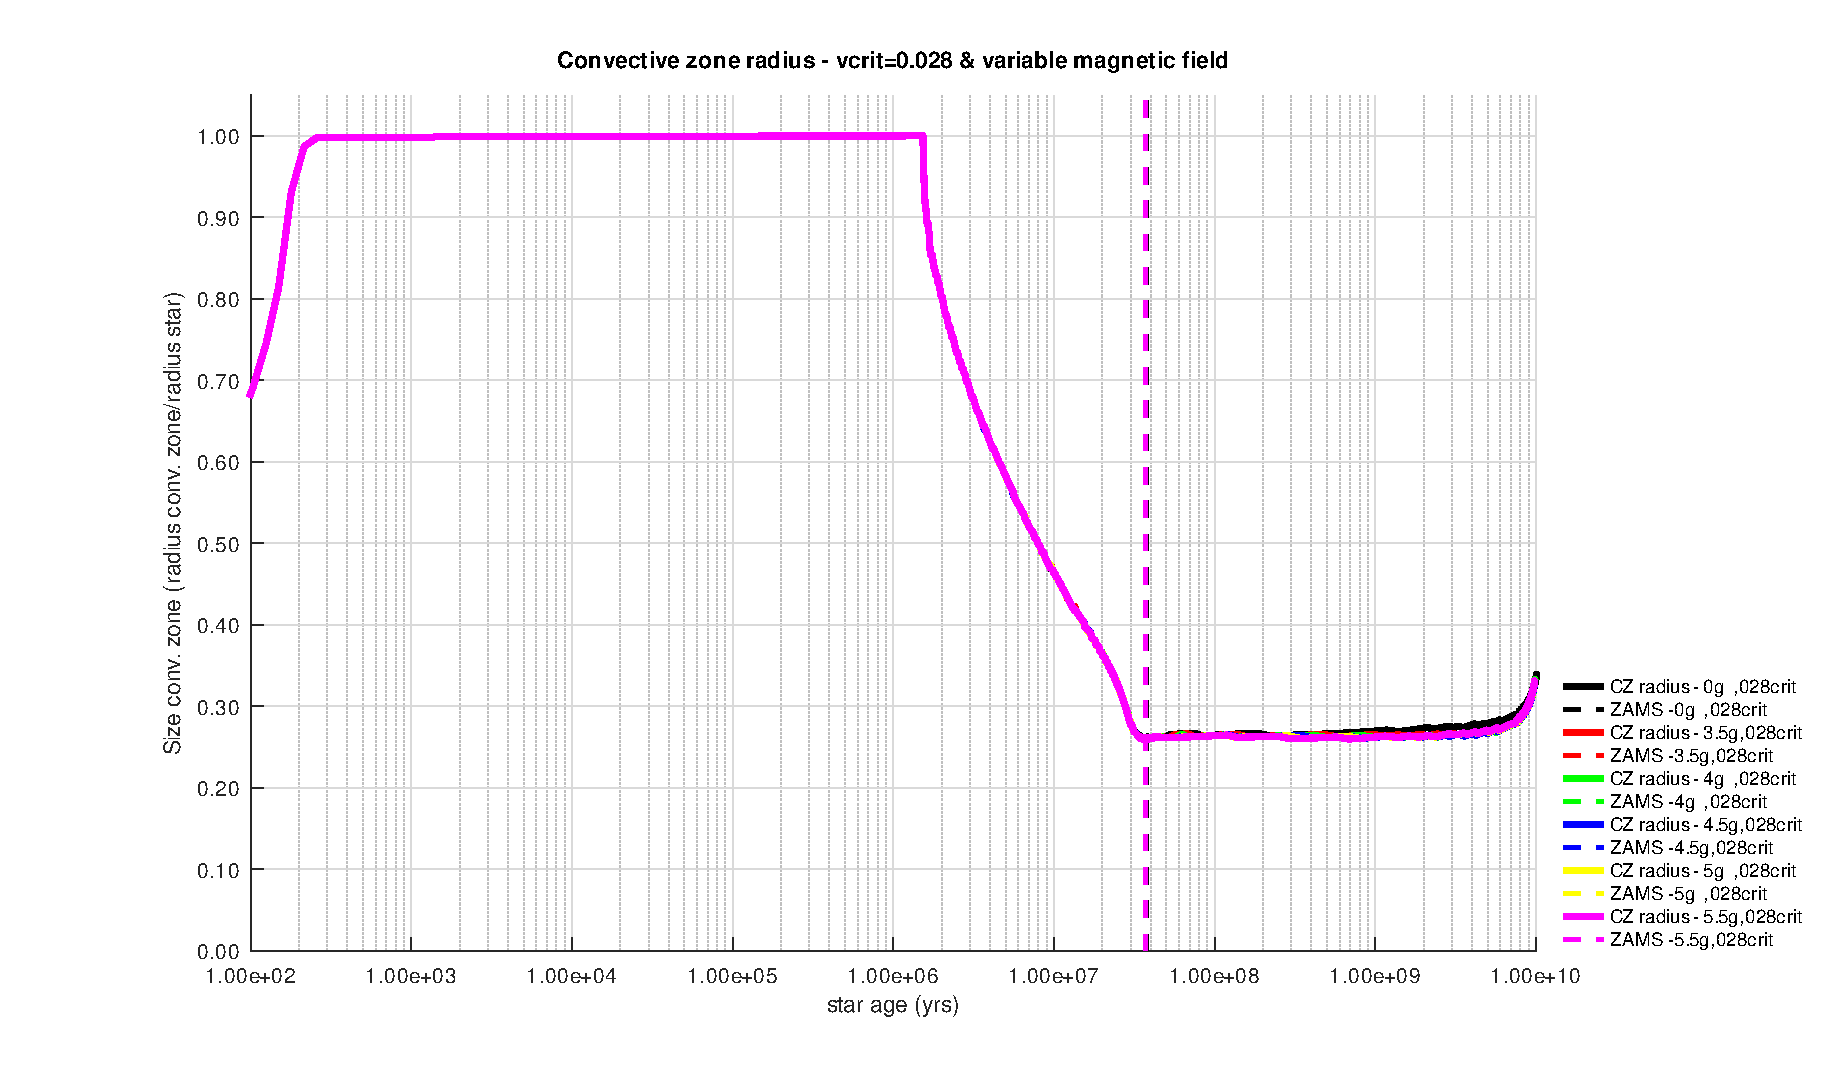
\includegraphics[width=\columnwidth]{figures/cz_vc_028_var_b.eps}
    \caption{The evolution of convective zone size, as a function of time for several 1 $M_{\sun}$ models. The models include a magnetic field with an intensity of 4G and PMS rotation with $v/v_{crit}$ between 0.0084 and 0.0336, respectively. Additionally it's simulated the magnetic braking effect of magnetic field with an intensity of 4G.The dashed lines make reference to the ZAMS.}
    \label{fig:cz_vc_028_var_b}
\end{figure}

\begin{figure}
	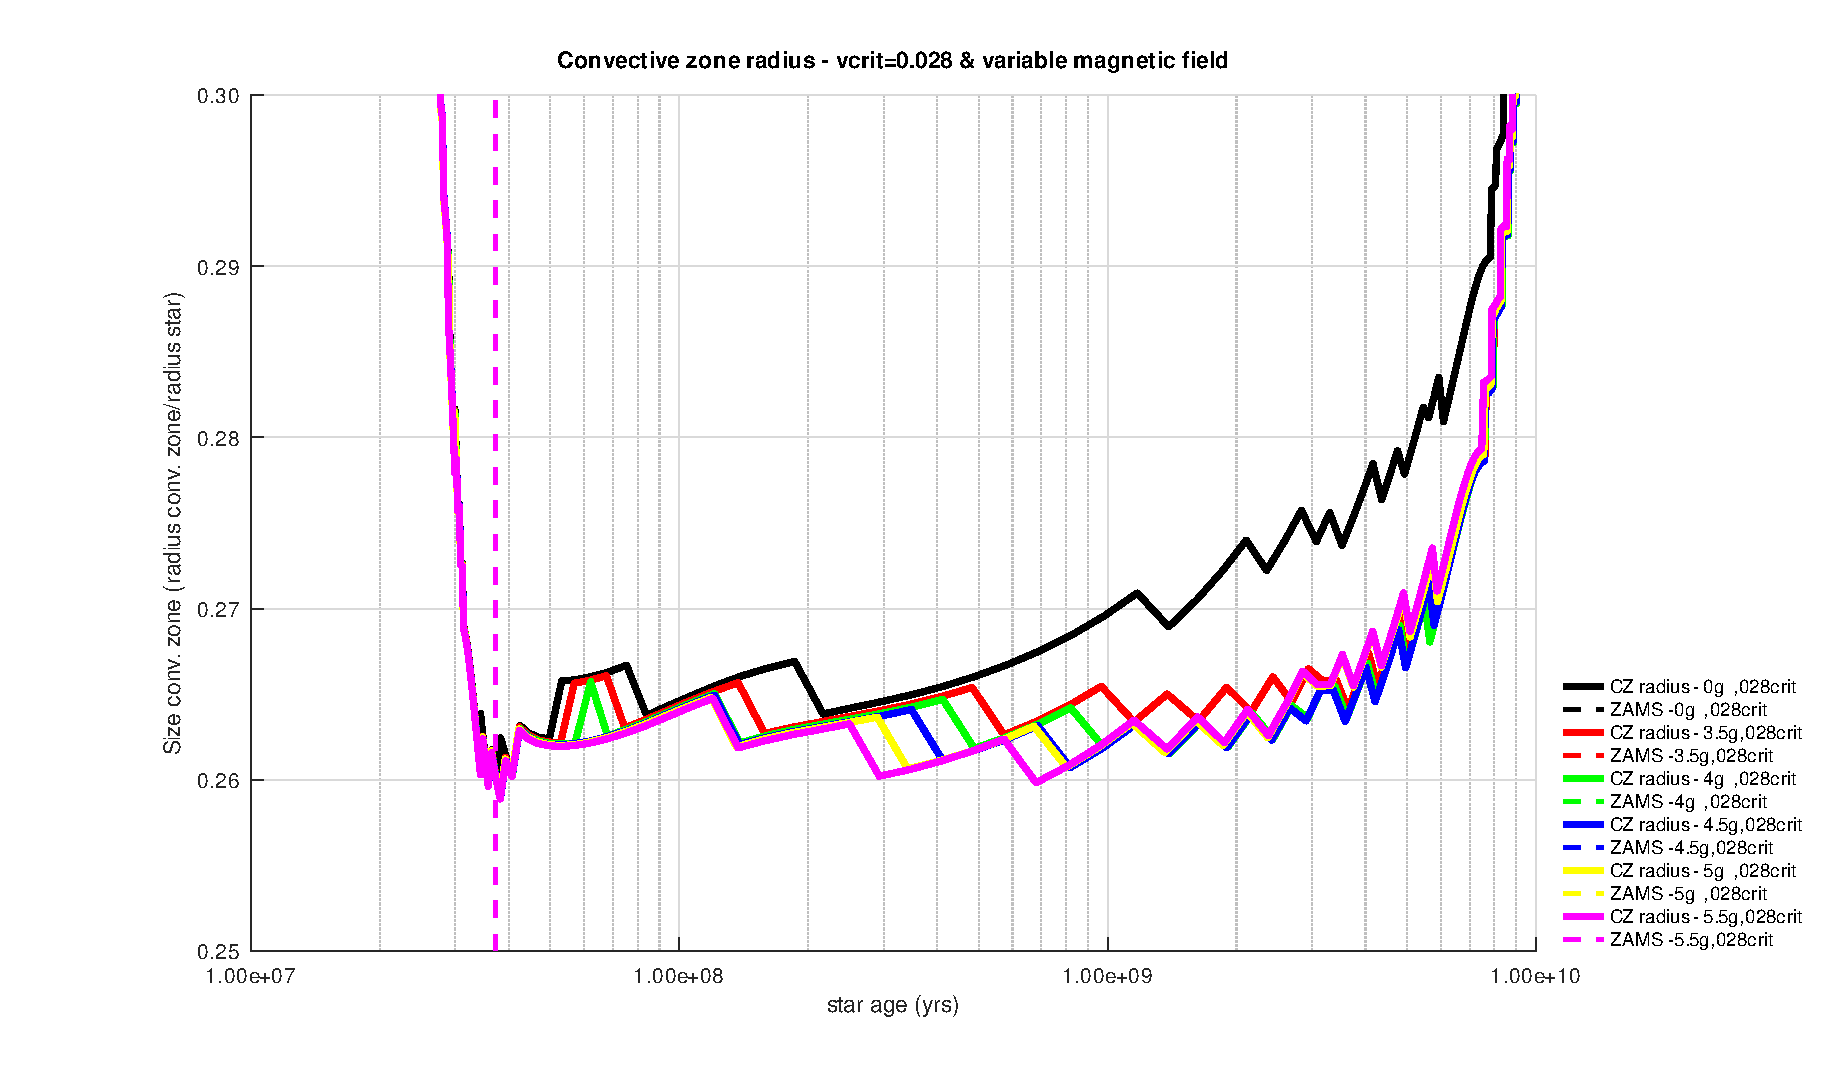
\includegraphics[width=\columnwidth]{figures/cz_vc_028_var_b_z1.eps}
    \caption{Similar to figure (\ref{fig:cz_vc_028_var_b}) but now showing in detail the convection zone size from the near ZAMS till the TAMS. As the intensity of the magnetic field increases, the size of the convective zone decreases.}
    \label{fig:cz_vc_028_var_b_z1}
\end{figure}

Before ending this section we would also like to comment on the other factor that directly affects AML; the loss of mass, $\Dot{M}$. In figure (\ref{fig:mdot_vc_028_var_b}) we can see the evolution of $\Dot{M}$ during PMS and MS. In the first stages of PMS is where the greatest loss of mass is concentrated and this diminishes as it approaches the ZAMS. If we add to the scenario the fact that the star also decreases its radius during the PMS we have as a result that the star increases $\Omega$ obeying the principle of conservation of angular momentum. When reaching the ZAMS, the radius of the star remains more or less stable for much of the MS (except for its final stage) but continues to lose mass so it continues to increase its angular velocity, although in a less aggressive way if we compare it with the PMS. However, as a consequence of both the appearance of the radiative core during Henyey track and the existence of a convective zone (see fig. (\ref{fig:mb_act_var_vel_vc_028})), the magnetic braking routine is activated, causing the angular velocity of the star to begin to decrease along the entire MS. The more intense the magnetic field, the greater the braking effect.\par 

\begin{figure}
	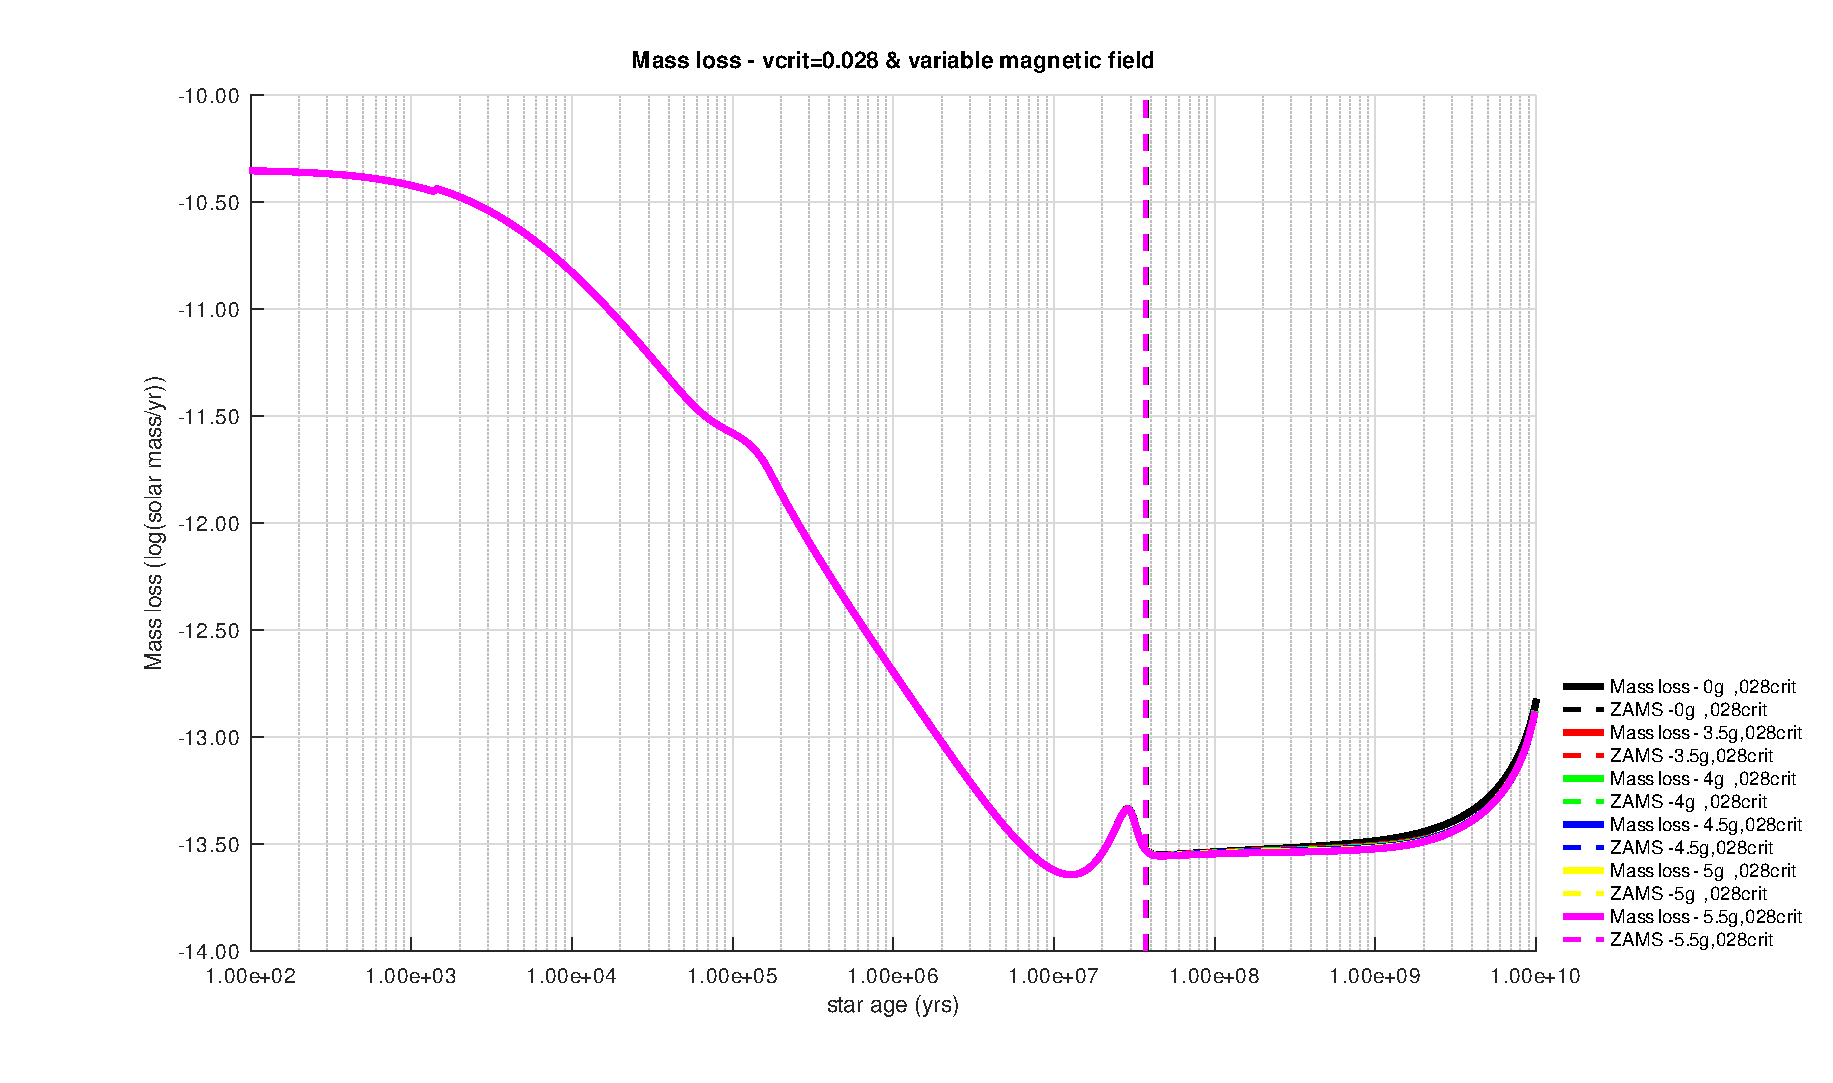
\includegraphics[width=\columnwidth]{figures/mdot_vc_028_var_b.eps}
    \caption{The evolution of mass loss $\Dot{M}$ , as a function of time for several 1 $M_{\sun}$ models. The models include a variable magnetic field intensity between 0G and 5.5G and PMS rotation with $v/v_{crit}=0.028$. The dashed lines make reference to the ZAMS.}
    \label{fig:mdot_vc_028_var_b}
\end{figure}

\begin{figure}
	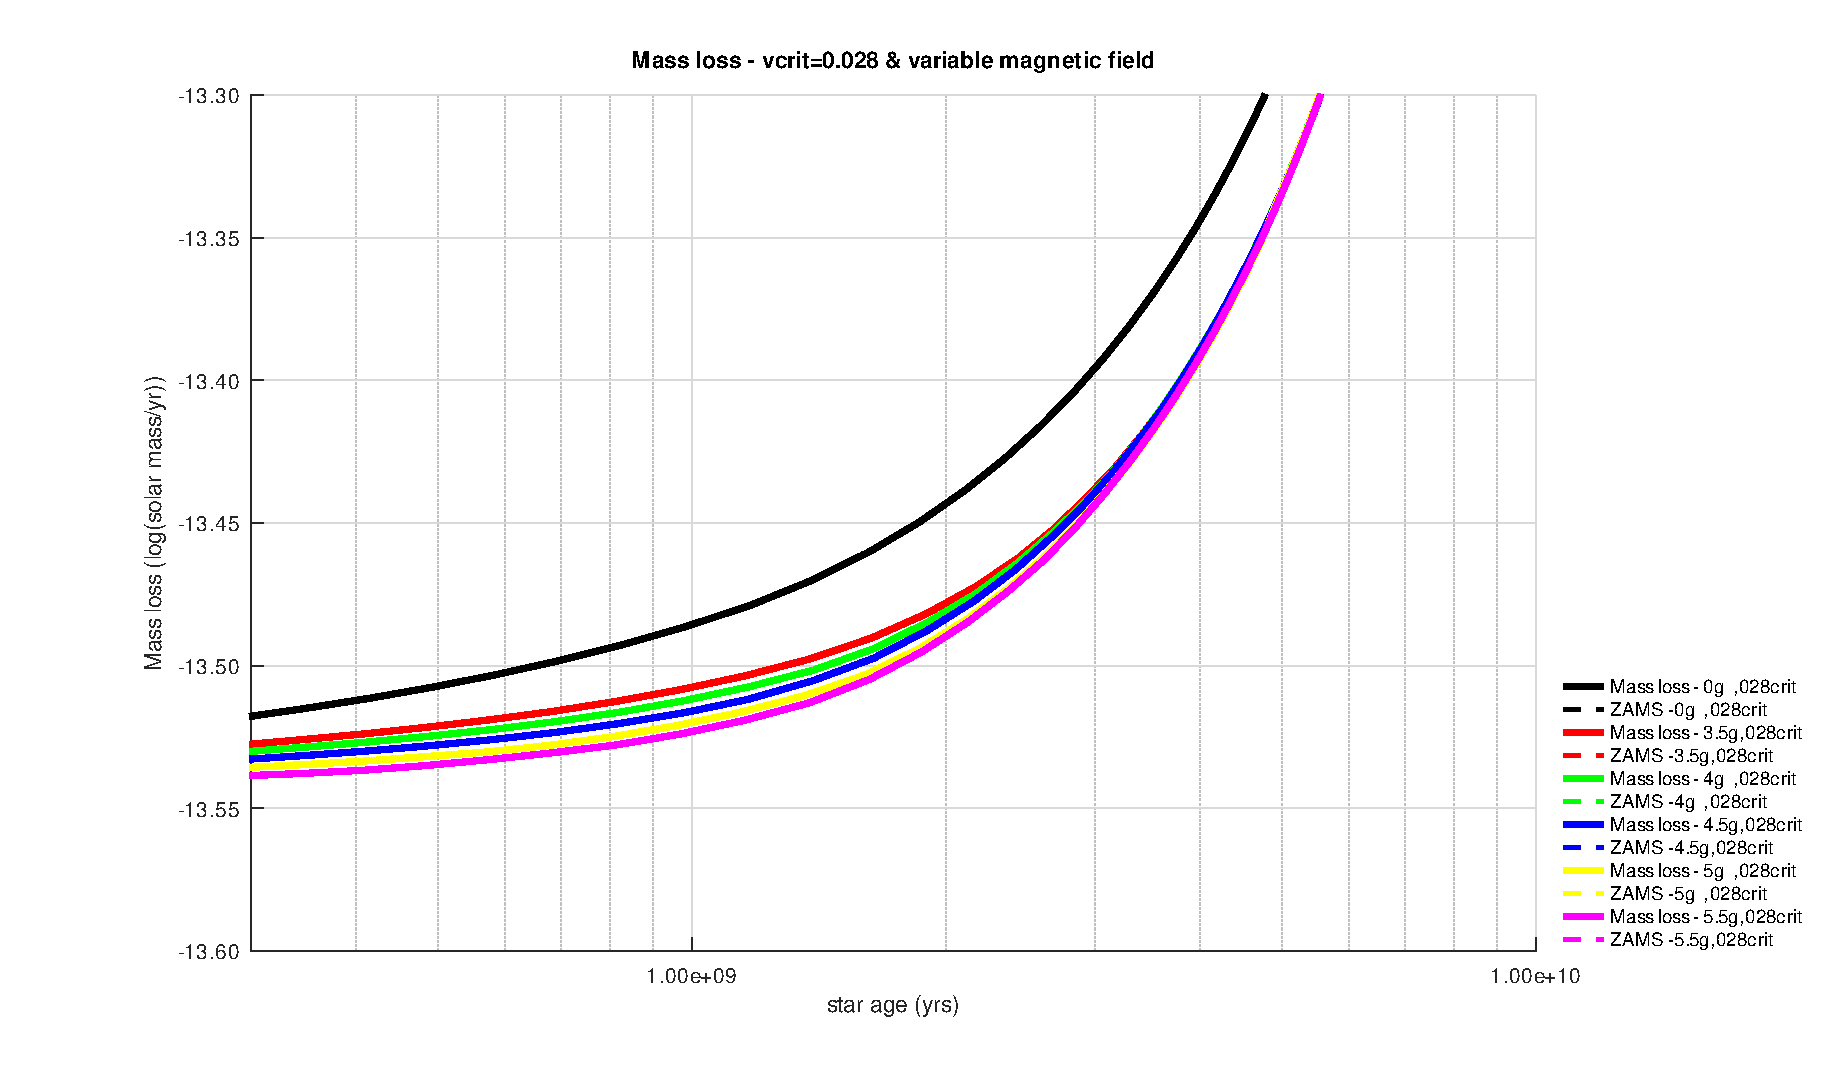
\includegraphics[width=\columnwidth]{figures/mdot_vc_028_var_b_z1.eps}
    \caption{The evolution of mass loss $\Dot{M}$ as the star is approaching TAMS, as a function of time for several 1 $M_{\sun}$ models. The models include a variable magnetic field intensity between 0G and 5.5G and PMS rotation with $v/v_{crit}=0.028$. The stronger the magnetic field, the lower both the angular velocity and $\Dot{M}$. The dashed lines make reference to the ZAMS.}
    \label{fig:mdot_vc_028_var_b_z1}
\end{figure}

\begin{figure}
	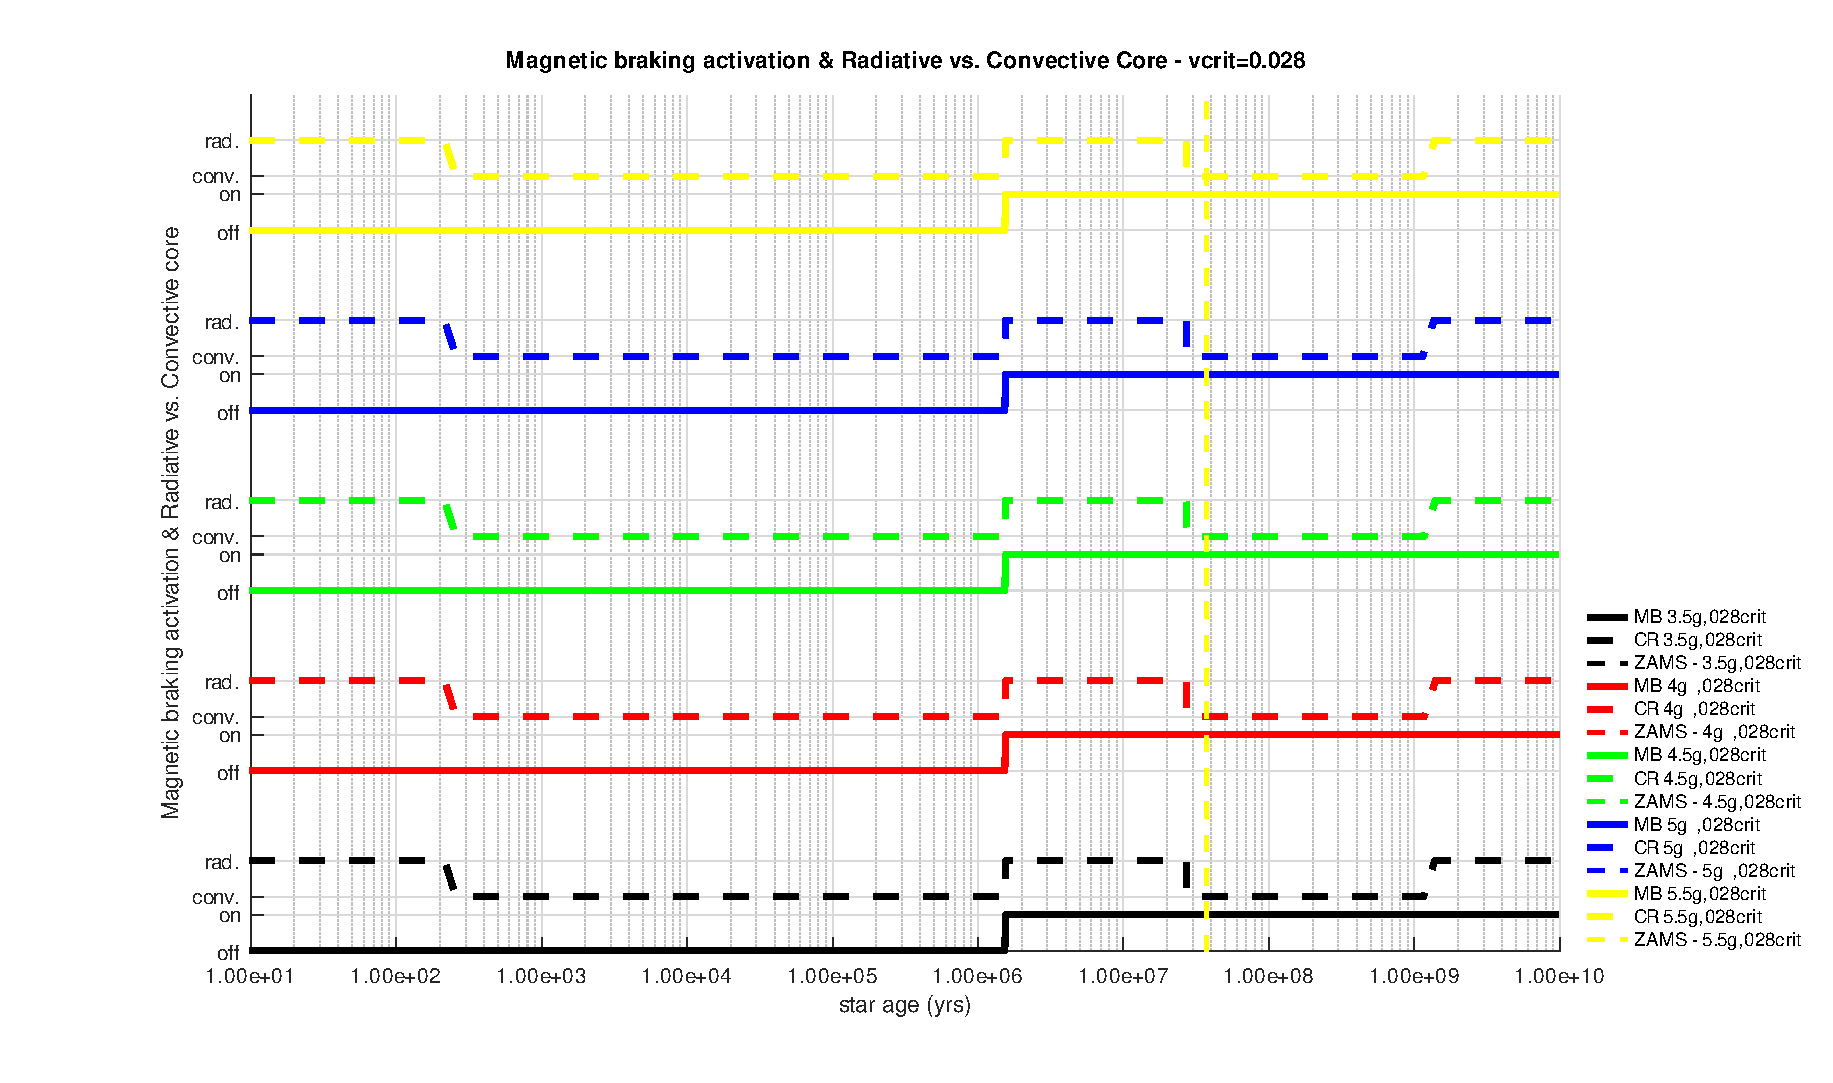
\includegraphics[width=\columnwidth]{figures/mb_act_var_vel_vc_028.eps}
    \caption{The evolution of convective zone size, as a function of time for several 1 $M_{\sun}$ models. The models include a magnetic field with an intensity of 4G and PMS rotation with $v/v_{crit}$ between 0.0084 and 0.0336, respectively. Additionally it's simulated the magnetic braking effect of magnetic field with an intensity of 4G. The solid lines signal the magnetic braking routine activation (on) and deactivation (off). The horizontal dashed lines inform about the star's core nature: radiative (rad) or convective (conv). The vertical dashed lines make reference to the ZAMS.}
    \label{fig:mb_act_var_vel_vc_028}
\end{figure}





\begin{figure*}
    \centering
    \begin{subfigure}[h]{0.47\textwidth}
    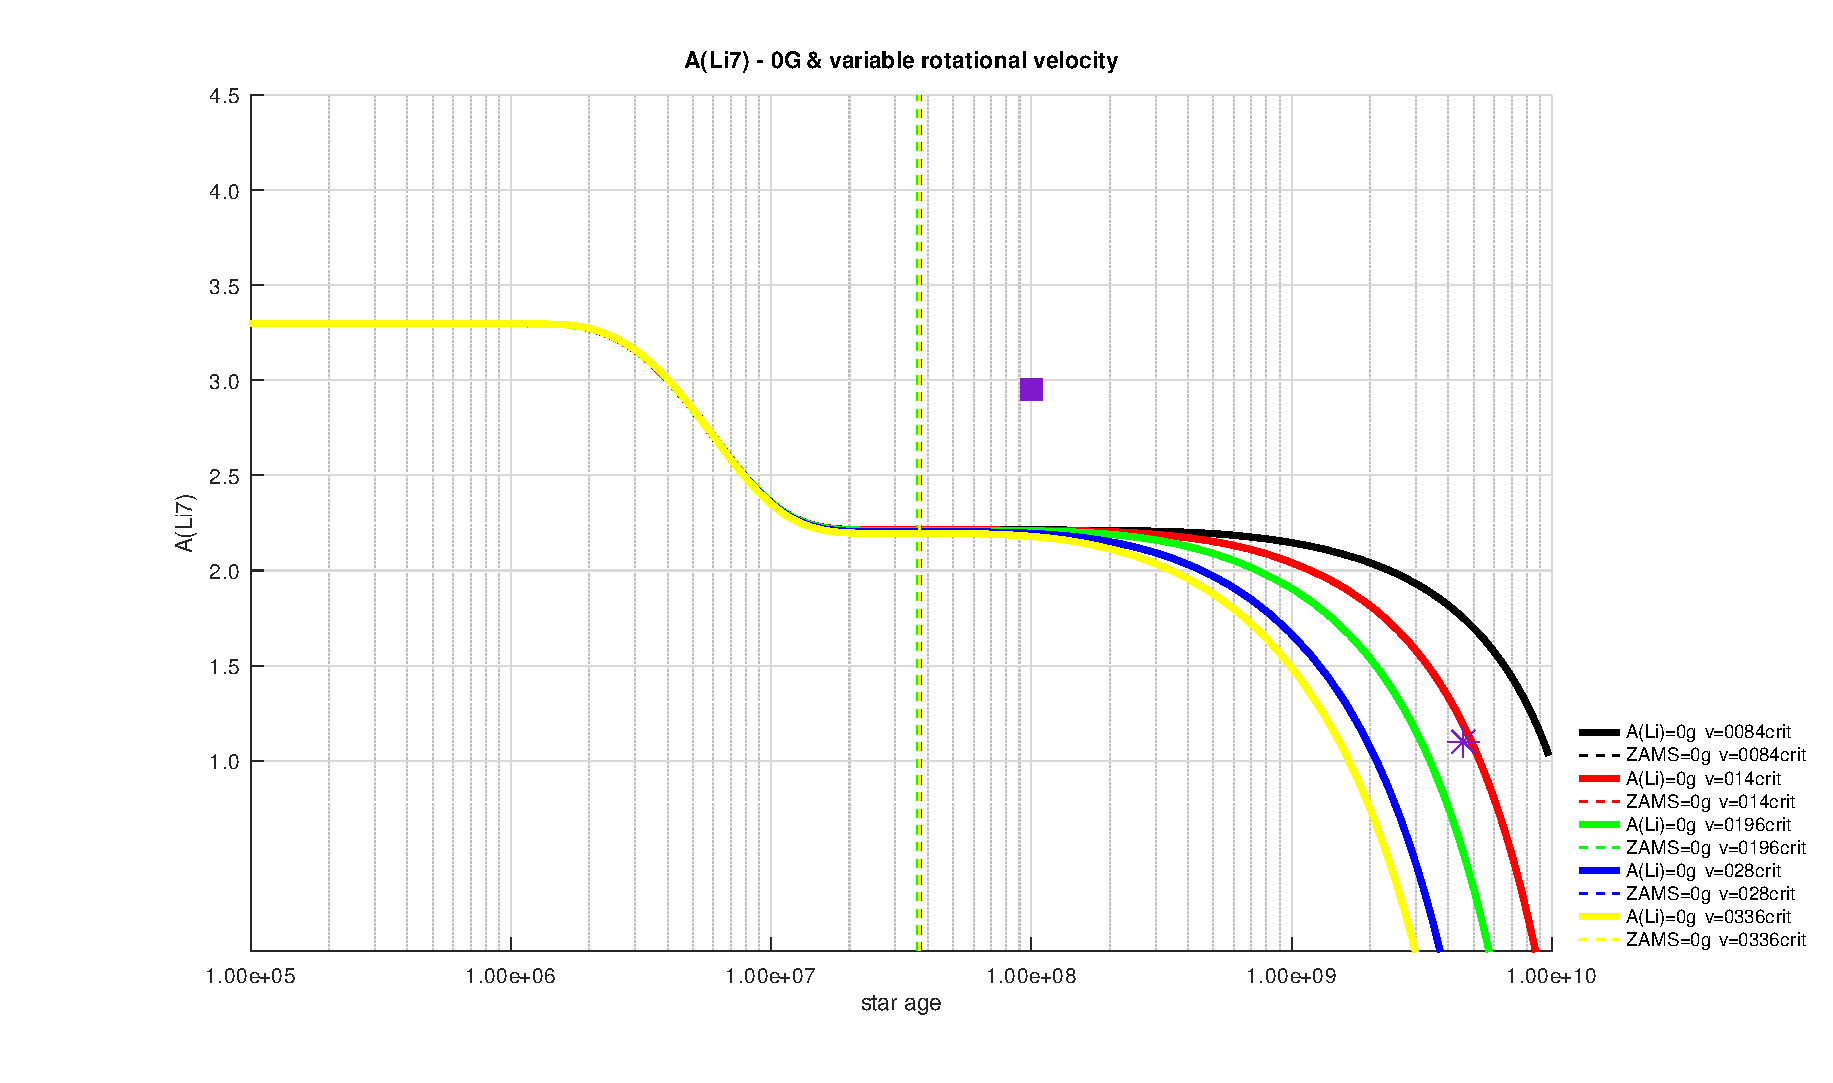
\includegraphics[width=\textwidth]{figures/li_var_vel_0_0g.eps}
    \label{fig:subim1}
    \end{subfigure}
    \begin{subfigure}[h]{0.47\textwidth}
    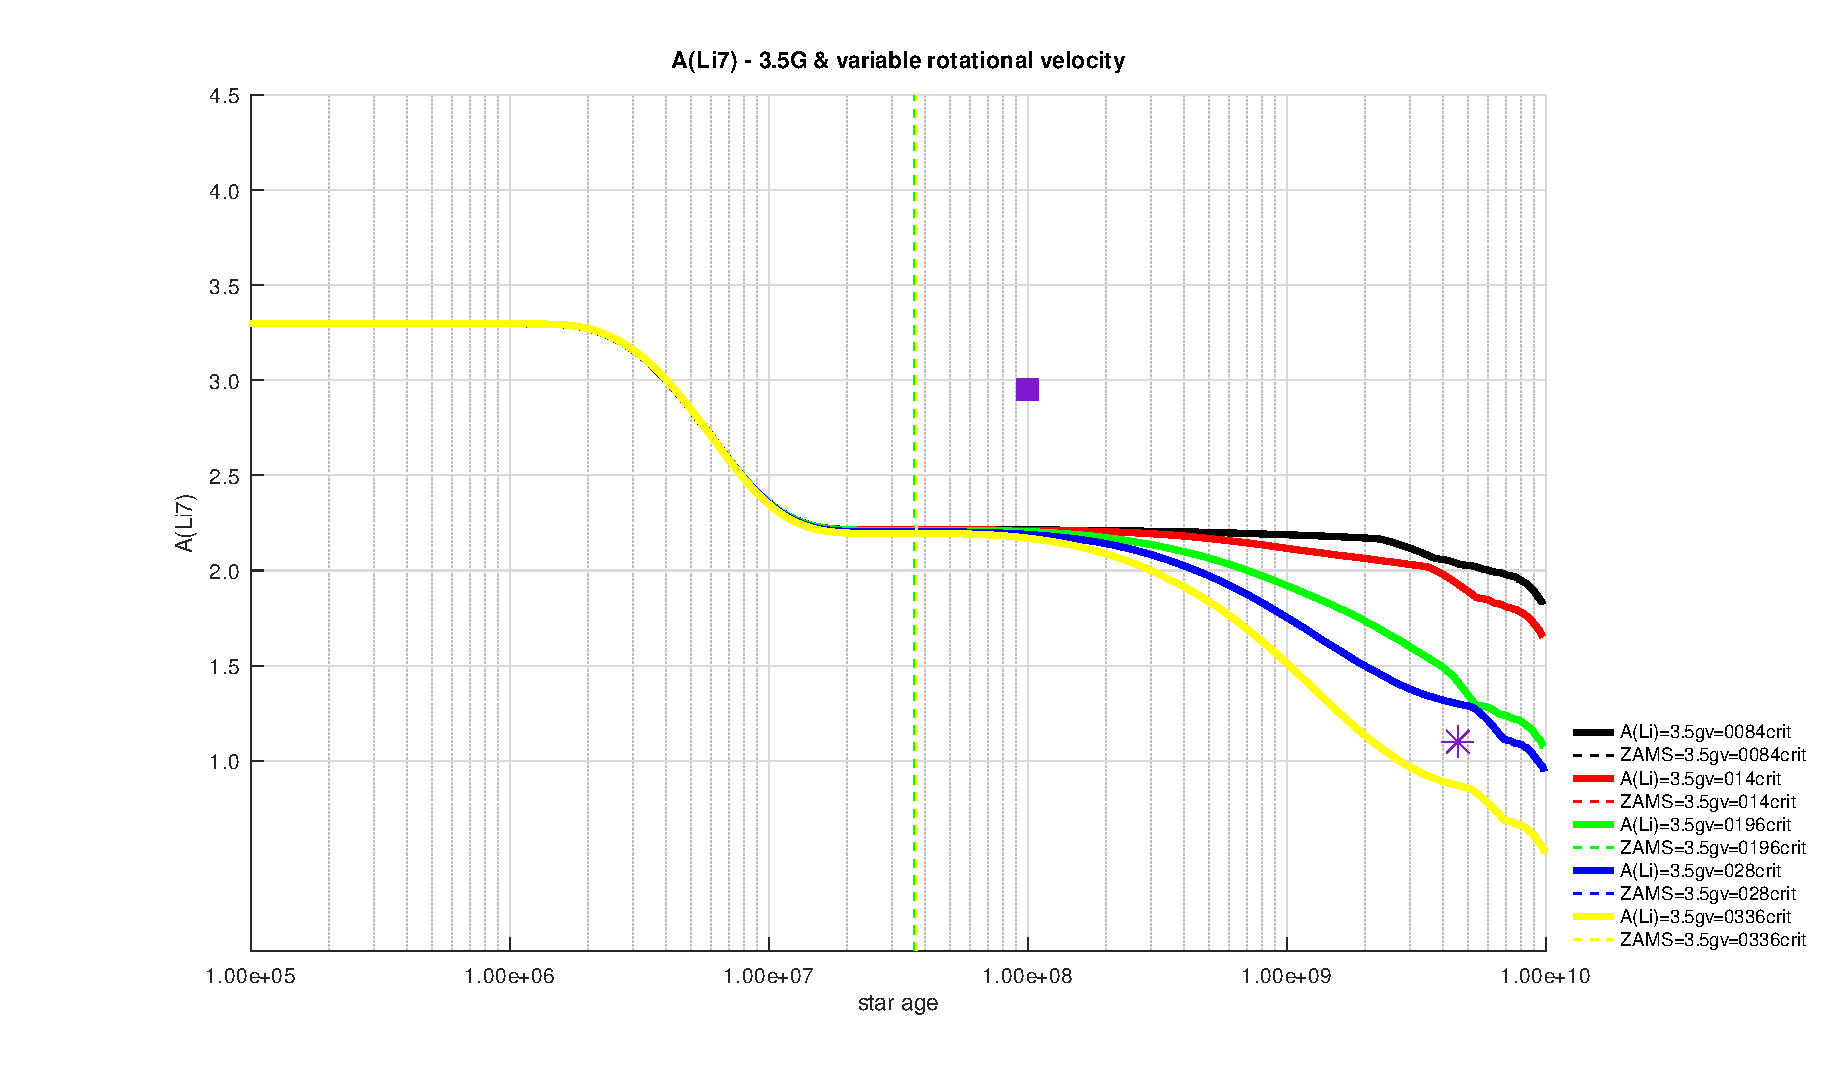
\includegraphics[width=\textwidth]{figures/li_var_vel_3_5g.eps}
    \label{fig:subim2}
    \end{subfigure}
    
    \begin{subfigure}[h]{0.47\textwidth}
    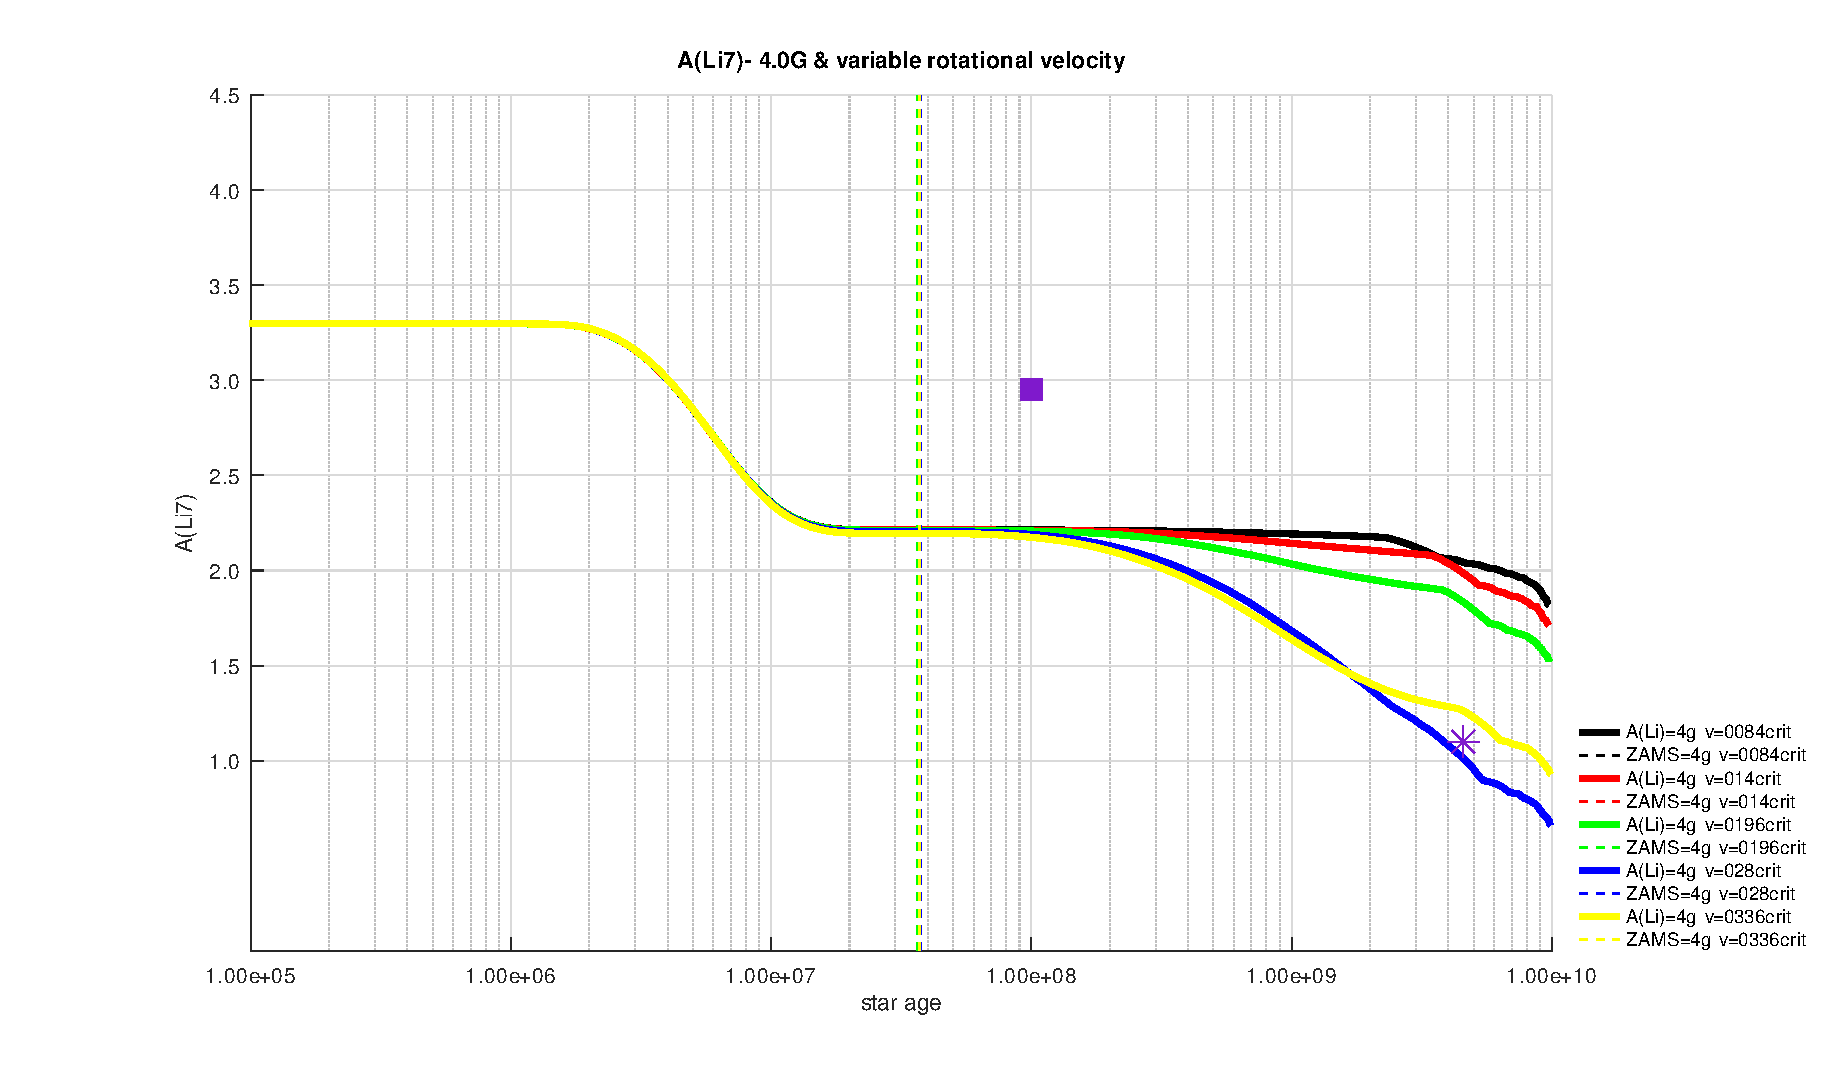
\includegraphics[width=\textwidth]{figures/li_var_vel_4_0g.eps}
    \label{fig:subim3}
    \end{subfigure}
    \begin{subfigure}[h]{0.47\textwidth}
    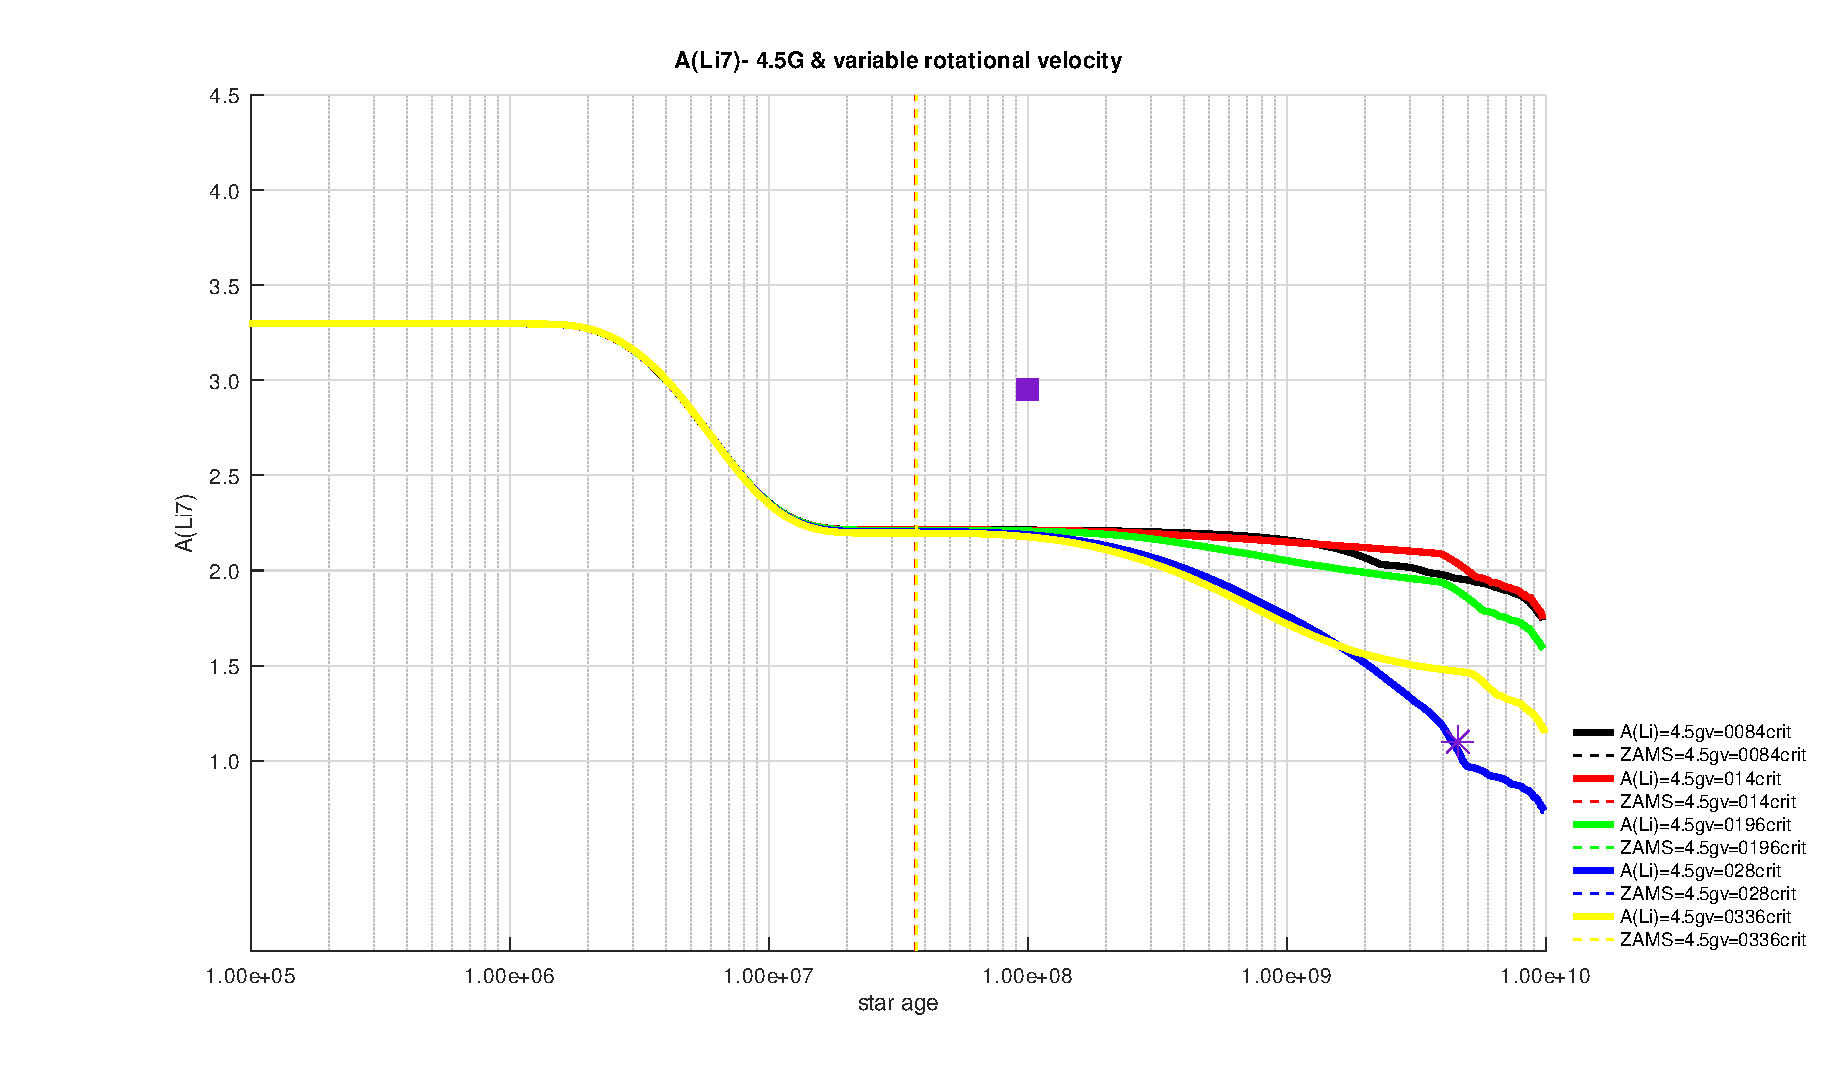
\includegraphics[width=\textwidth]{figures/li_var_vel_4_5g.eps}
    \label{fig:subim4}
    \end{subfigure}
    
    \begin{subfigure}[h]{0.47\textwidth}
    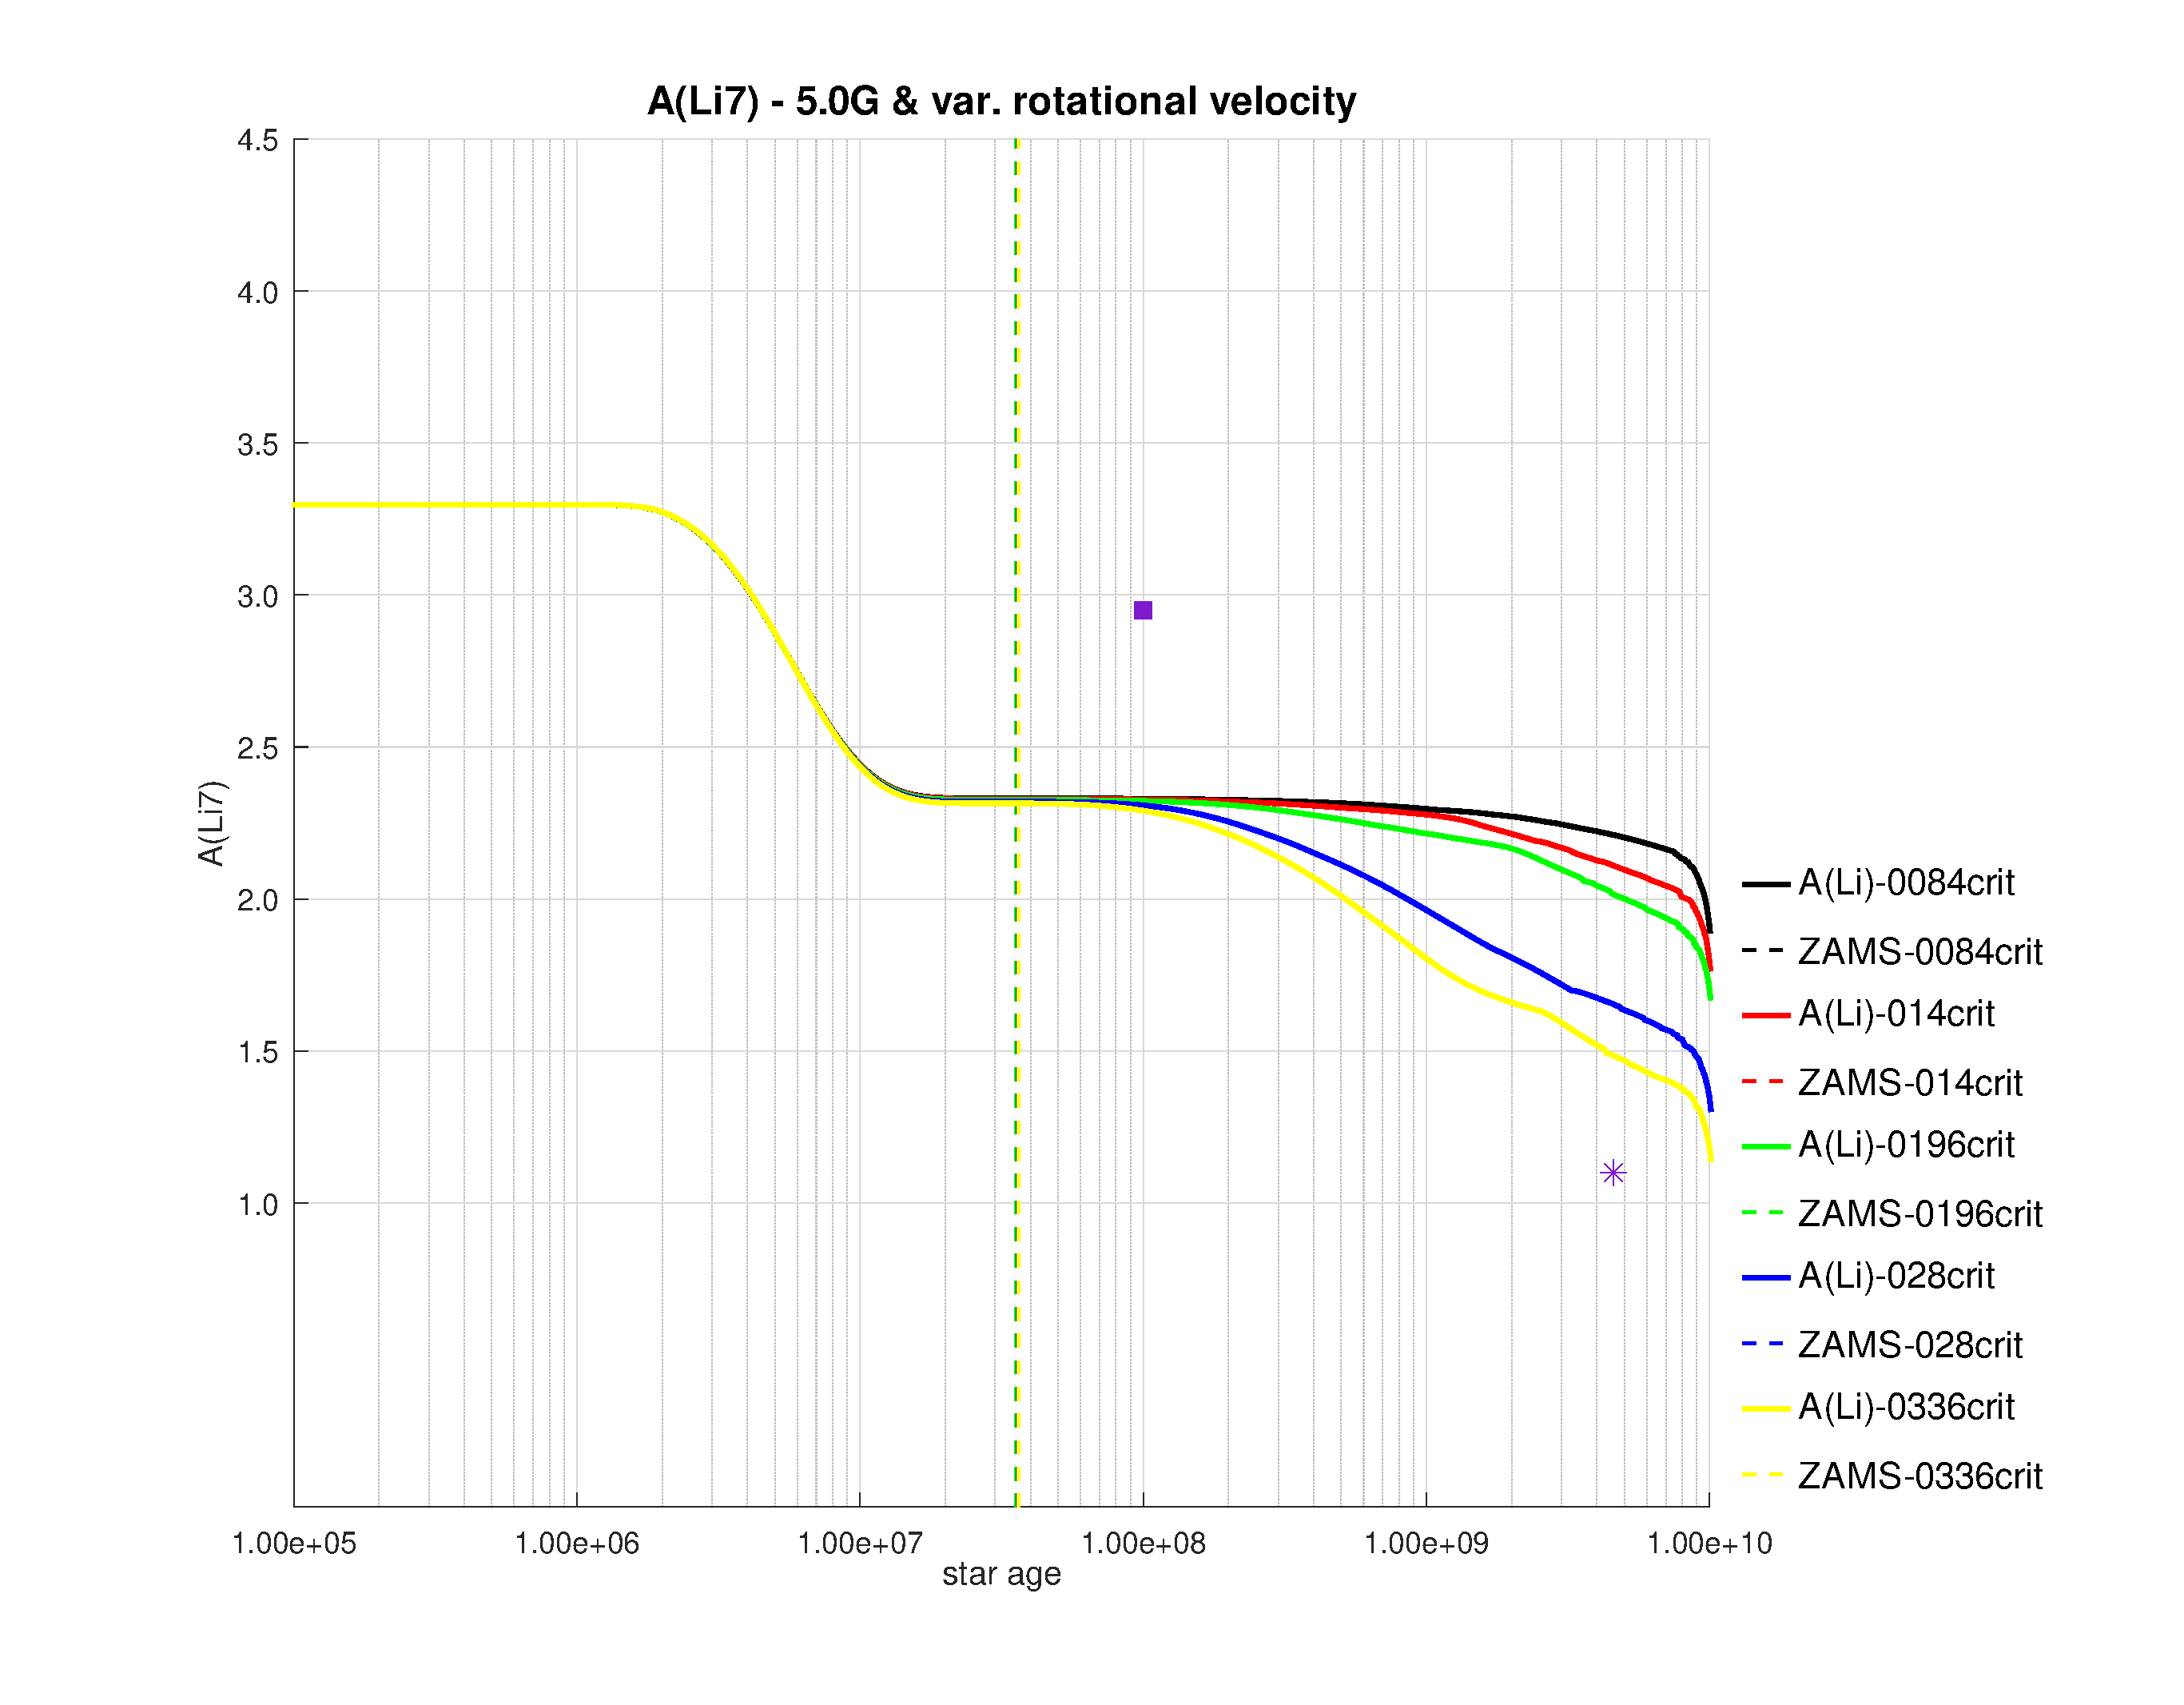
\includegraphics[width=\textwidth]{figures/li_var_vel_5_0g.eps}
    \label{fig:subim5}
    \end{subfigure}
    \begin{subfigure}[h]{0.47\textwidth}
    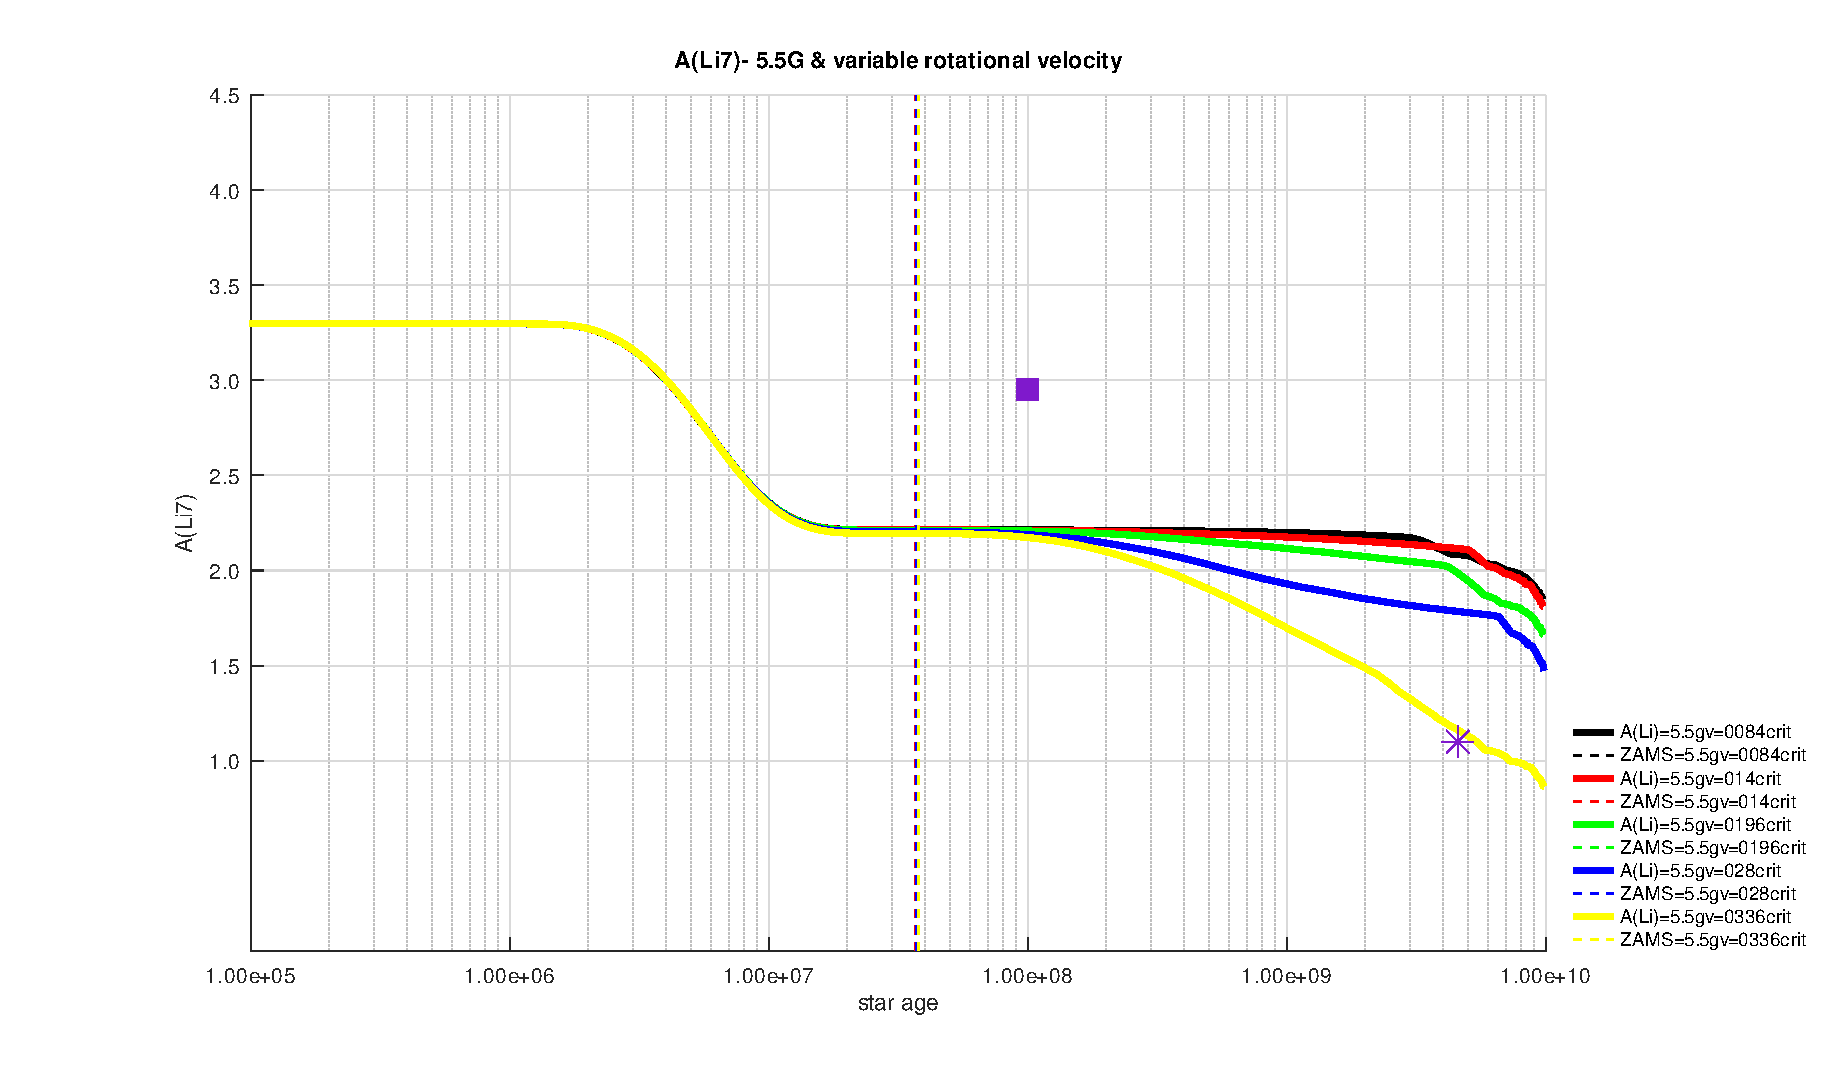
\includegraphics[width=\textwidth]{figures/li_var_vel_5_5g.eps}
    \label{fig:subim6}
    \end{subfigure}
\caption{The evolution of surface rotational velocity, as a function of time for several 1 $M_{\sun}$ models. The lines are models with includes PMS rotation with $v/v_{crit}$ between 0.0084 and 0.0336, respectively. The purple star is the surface Li abundance for the present-day Sun \citep{Asplund2009}. The dashed lines make reference to the ZAMS defined as the temporal simulation instant closest to the timestep in which both the central H mass fraction has been reduced by 0.0015 from its initial value and the model first $L_H/L_{phot} \geq 0.99$, where $L_{H}$ is luminosity produced by the H burning power at the star core and $L_{phot}$ represents the star luminosity in the photosphere.}
\label{fig:image2}
\end{figure*}
\par


\begin{figure*}
    \centering
    \begin{subfigure}[h]{0.47\textwidth}
    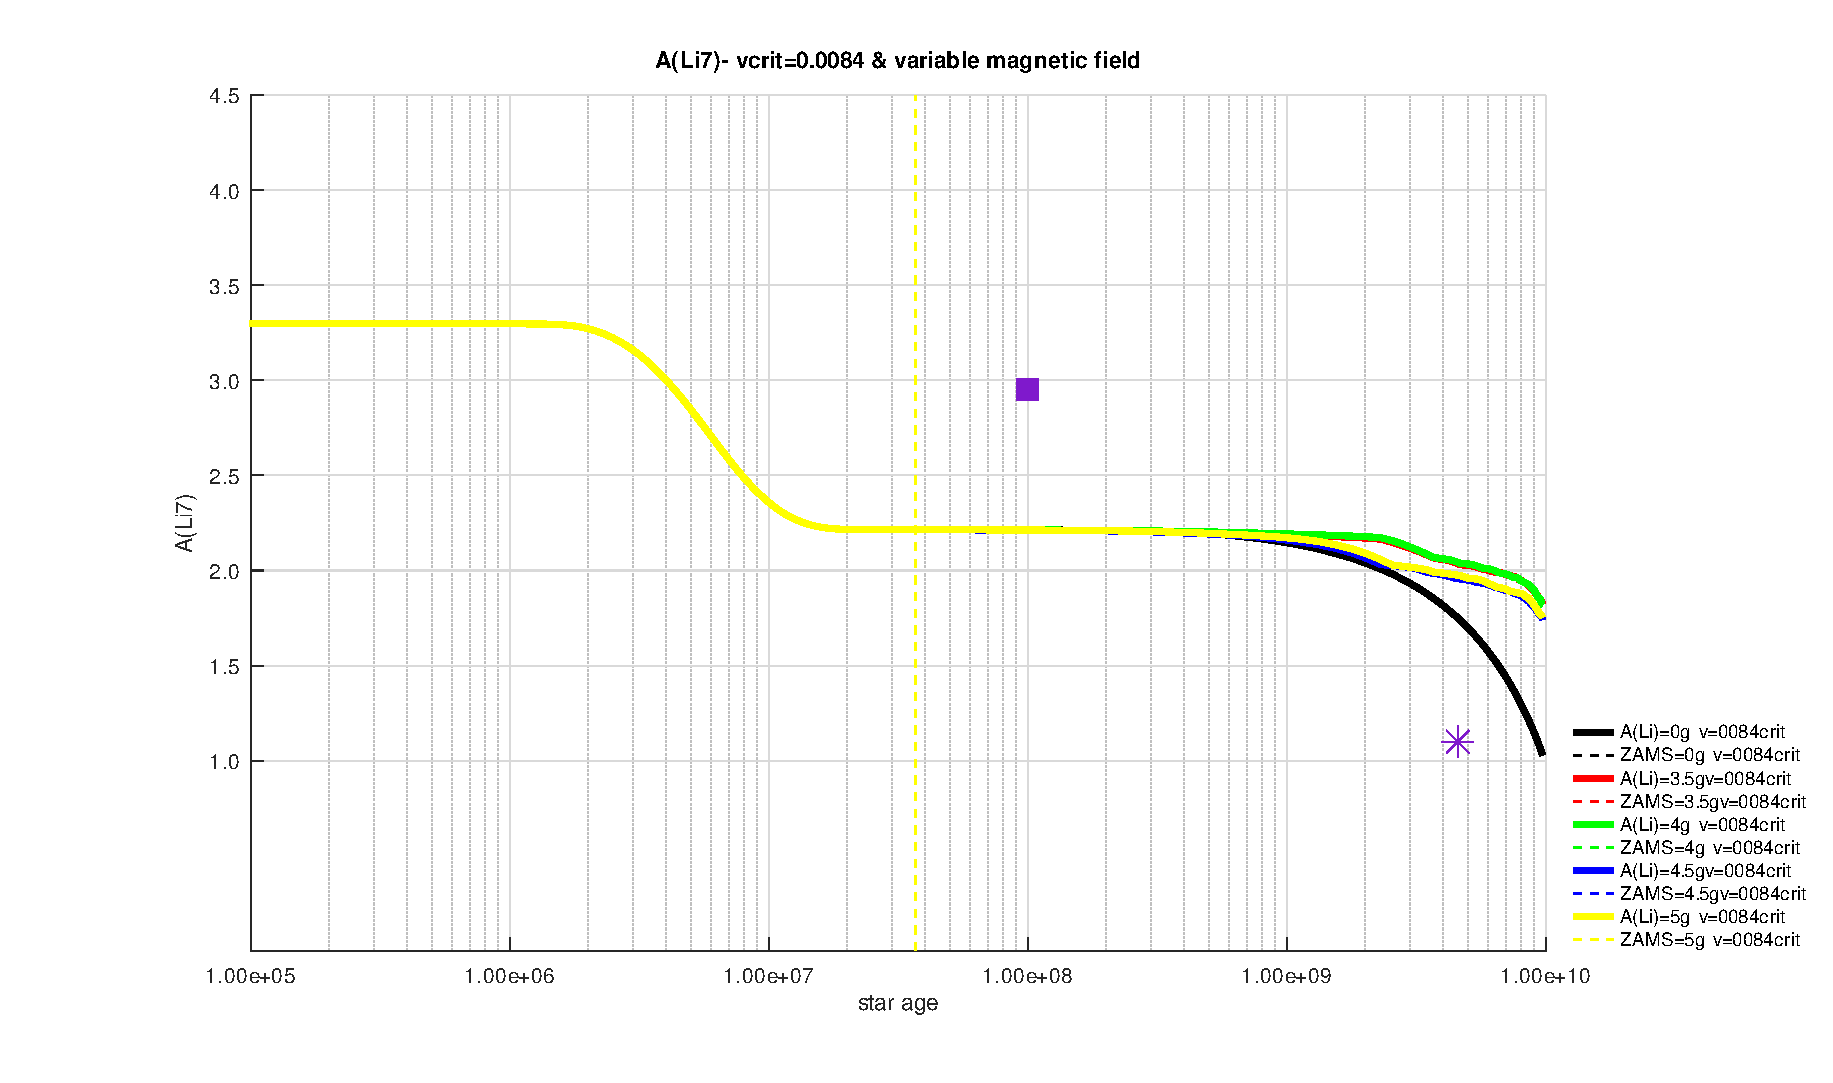
\includegraphics[width=\textwidth]{figures/li_vc_0084_var_b.eps}
    \label{fig:subim21}
    \end{subfigure}
    \begin{subfigure}[h]{0.47\textwidth}
    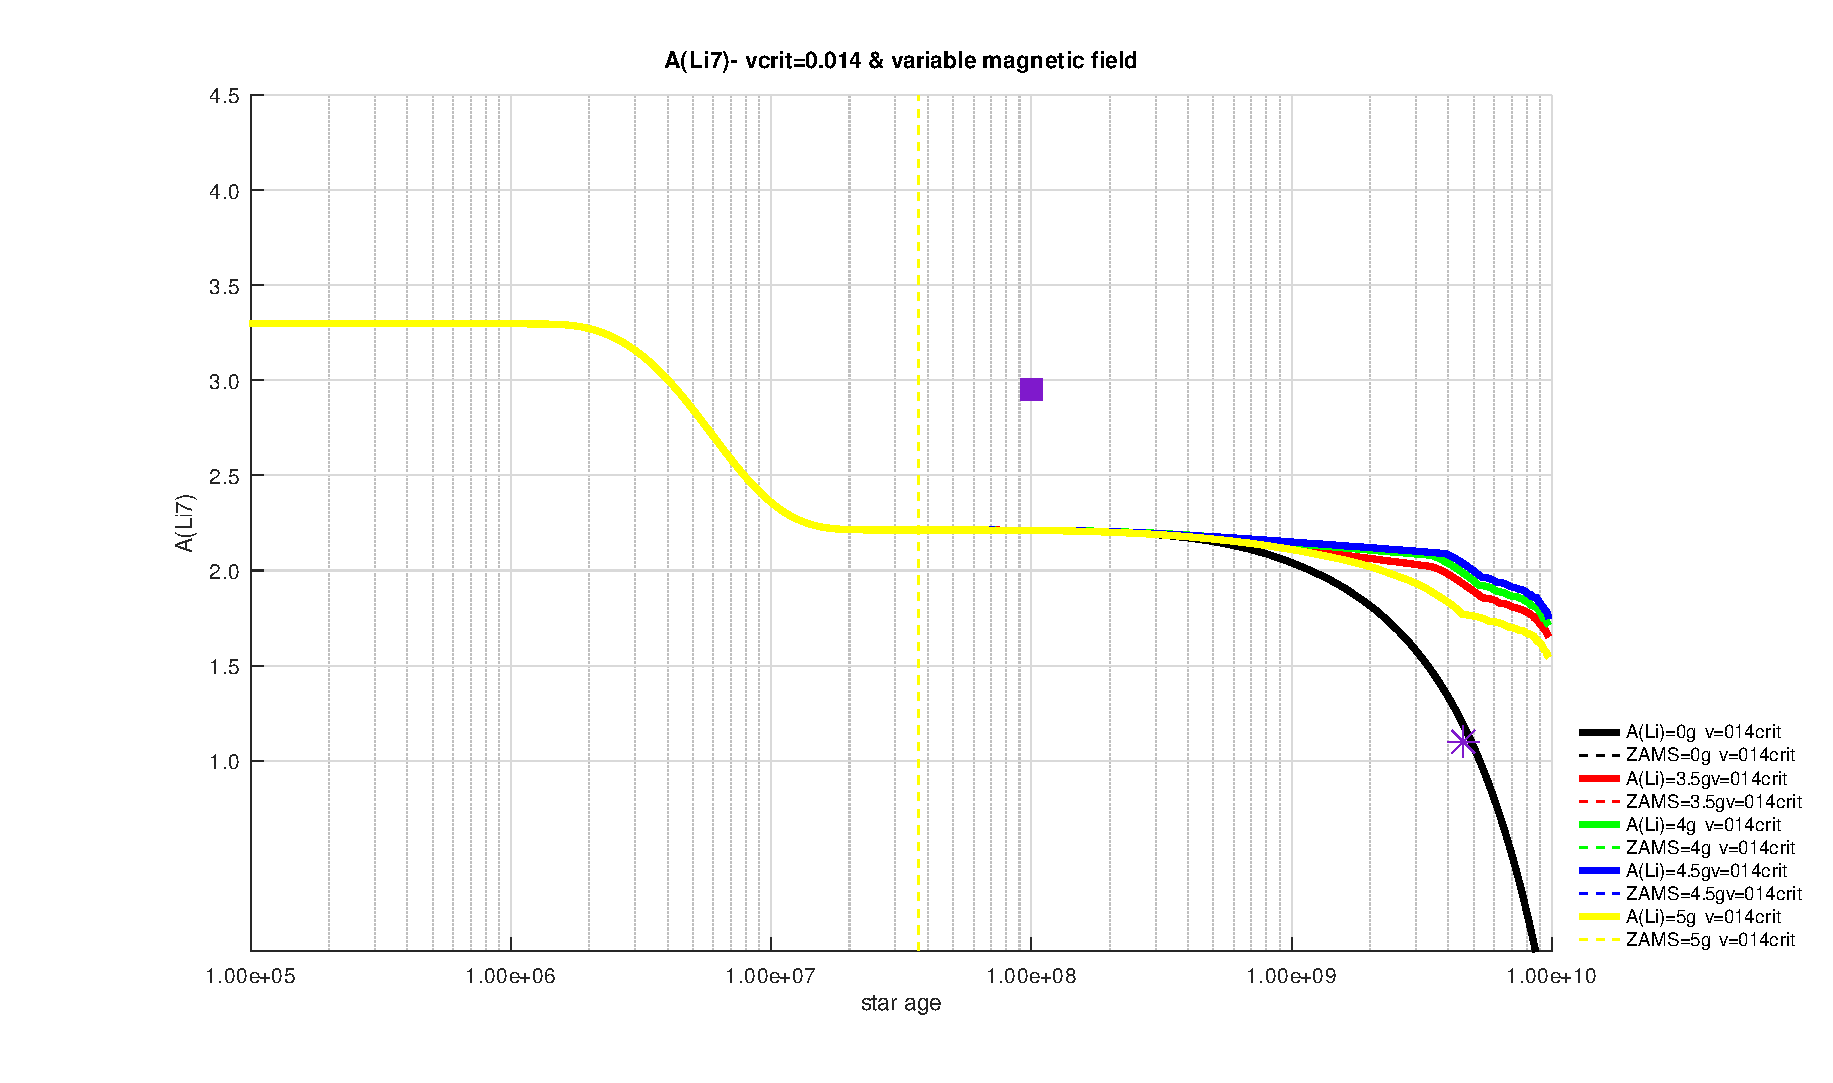
\includegraphics[width=\textwidth]{figures/li_vc_014_var_b.eps}
    \label{fig:subim22}
    \end{subfigure}
    \begin{subfigure}[h]{0.47\textwidth}
    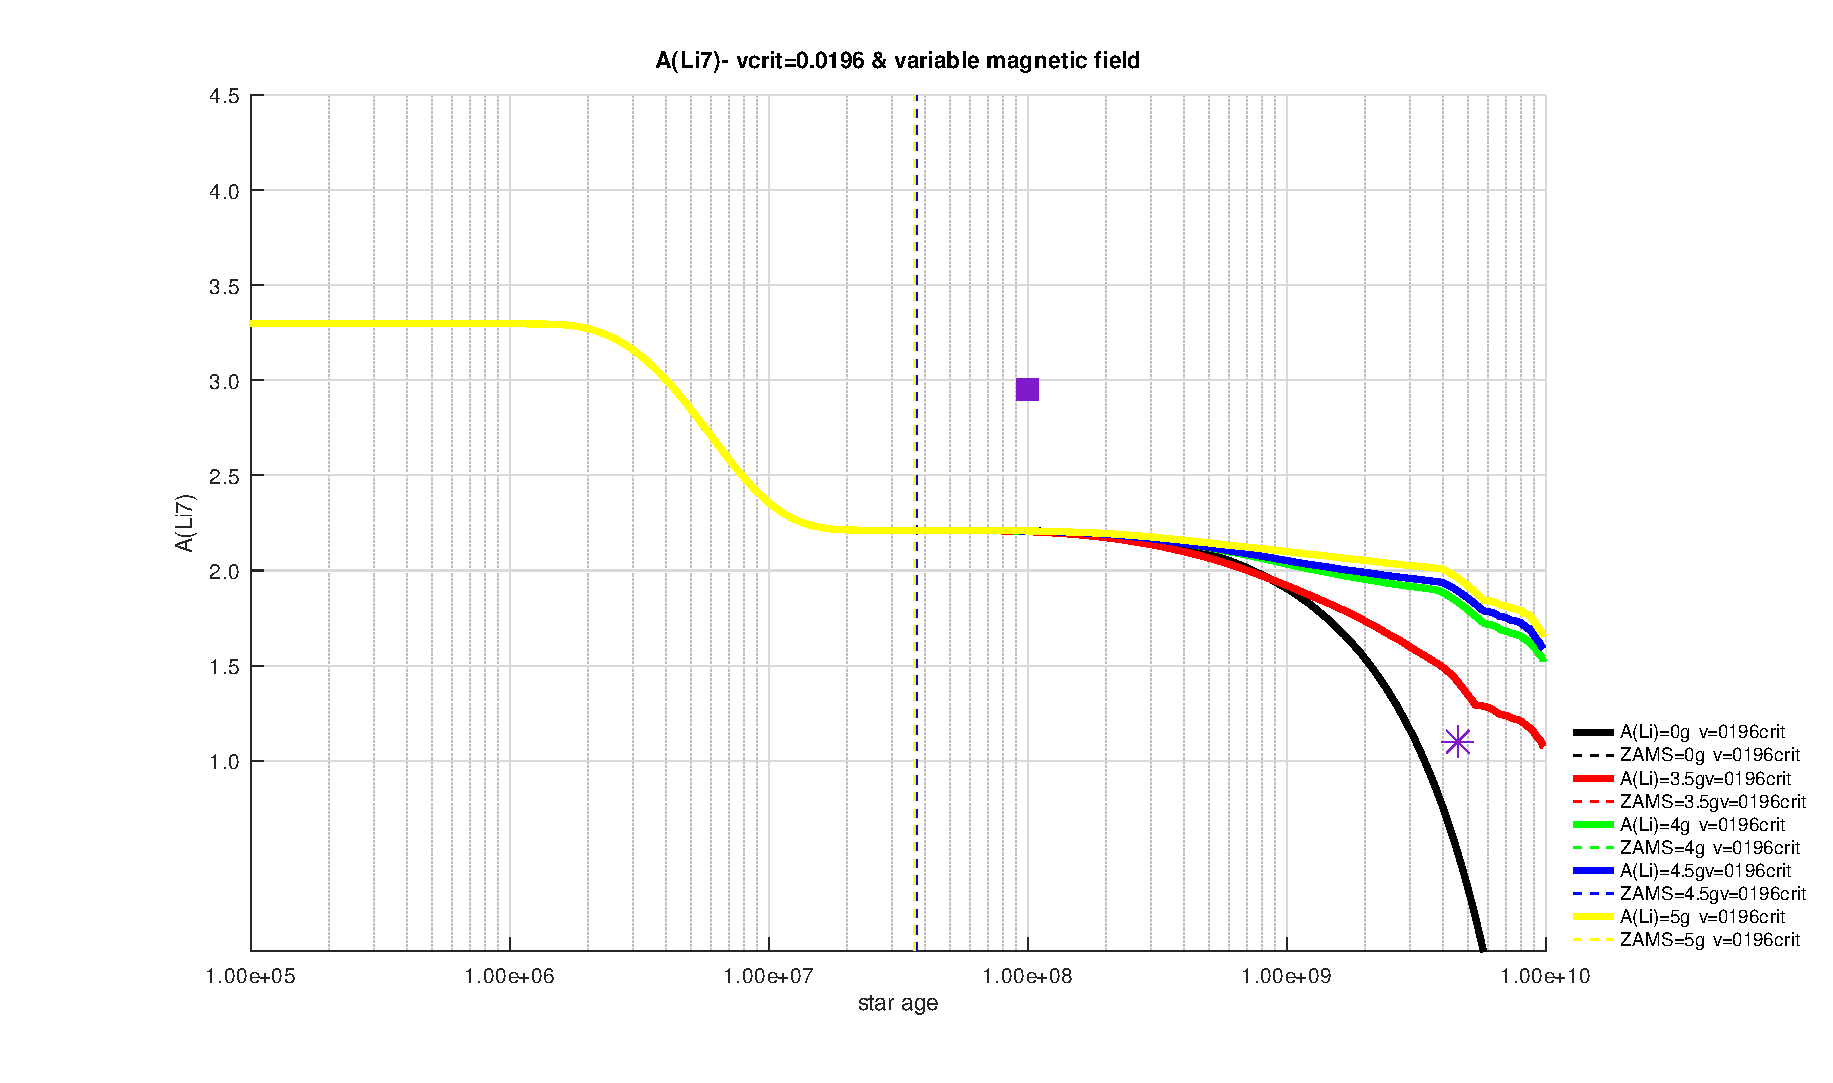
\includegraphics[width=\textwidth]{figures/li_vc_0196_var_b.eps}
    \label{fig:subim23}
    \end{subfigure}
    \begin{subfigure}[h]{0.47\textwidth}
    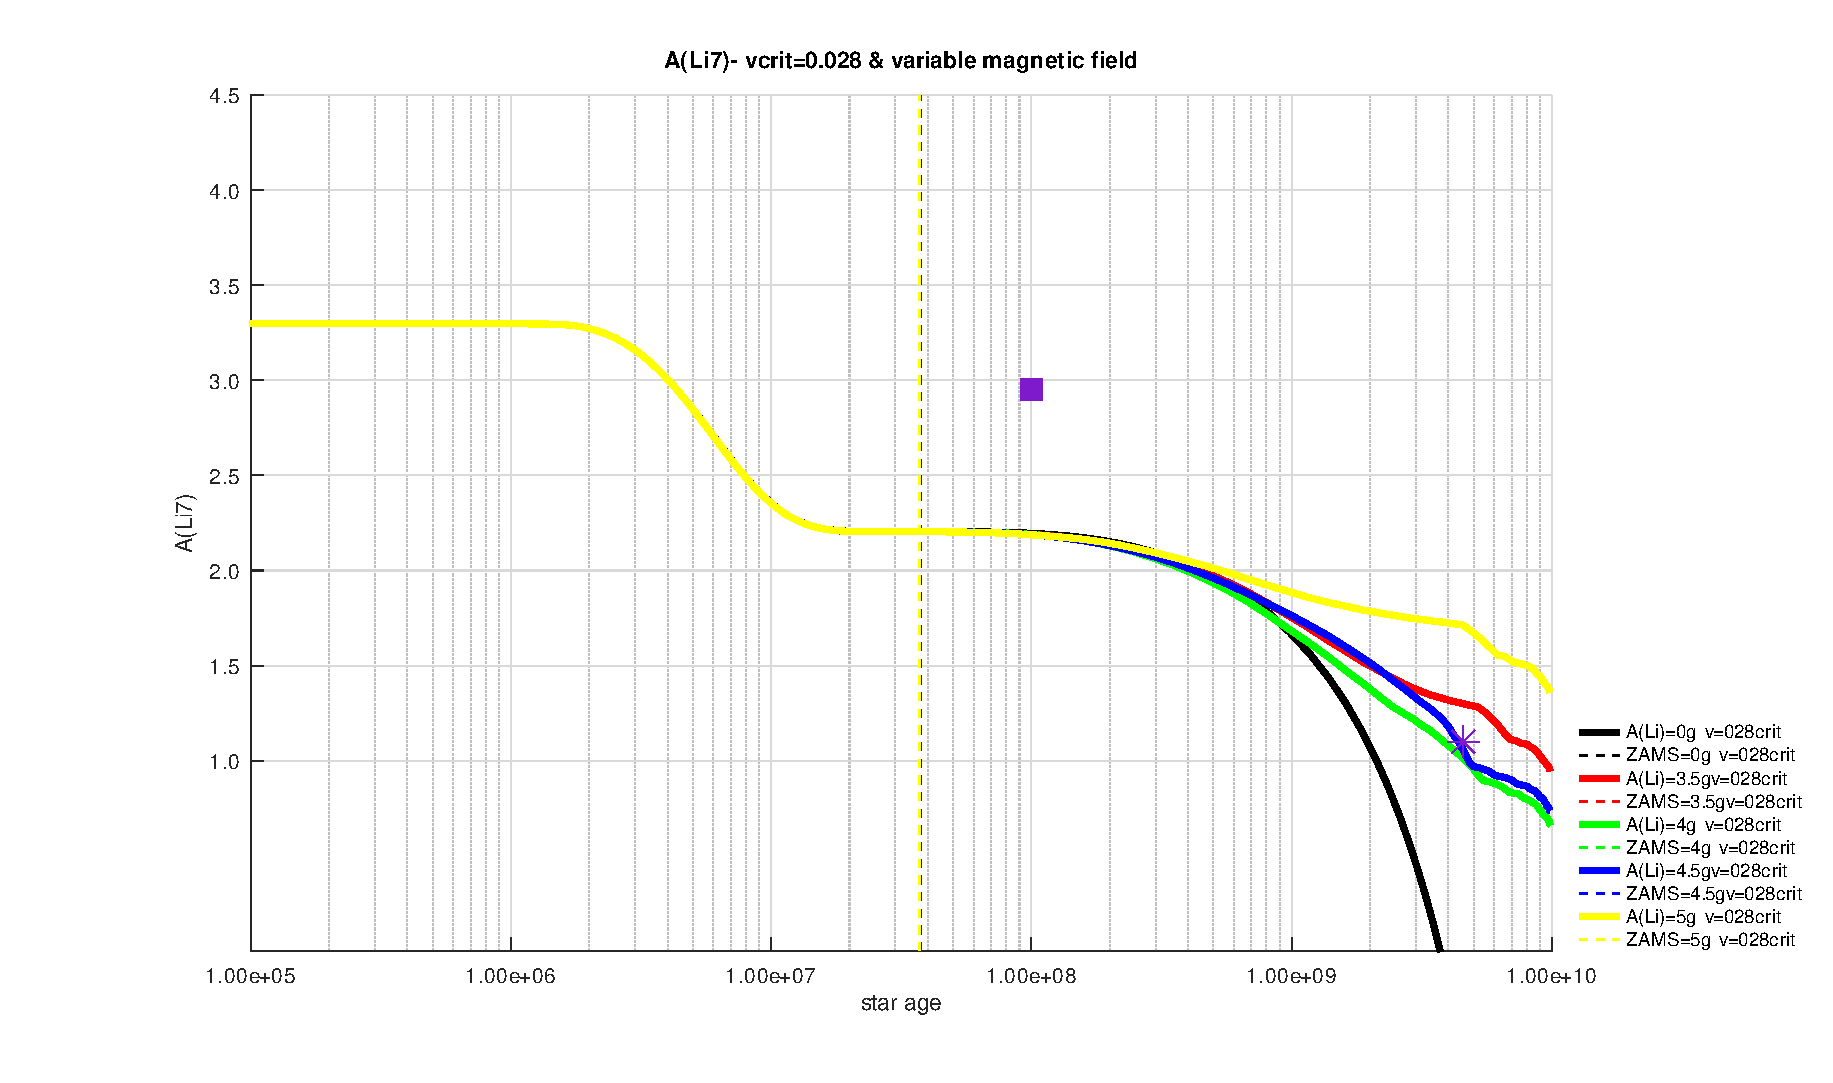
\includegraphics[width=\textwidth]{figures/li_vc_028_var_b.eps}
    \label{fig:subim24}
    \end{subfigure}
    \begin{subfigure}[h]{0.47\textwidth}
    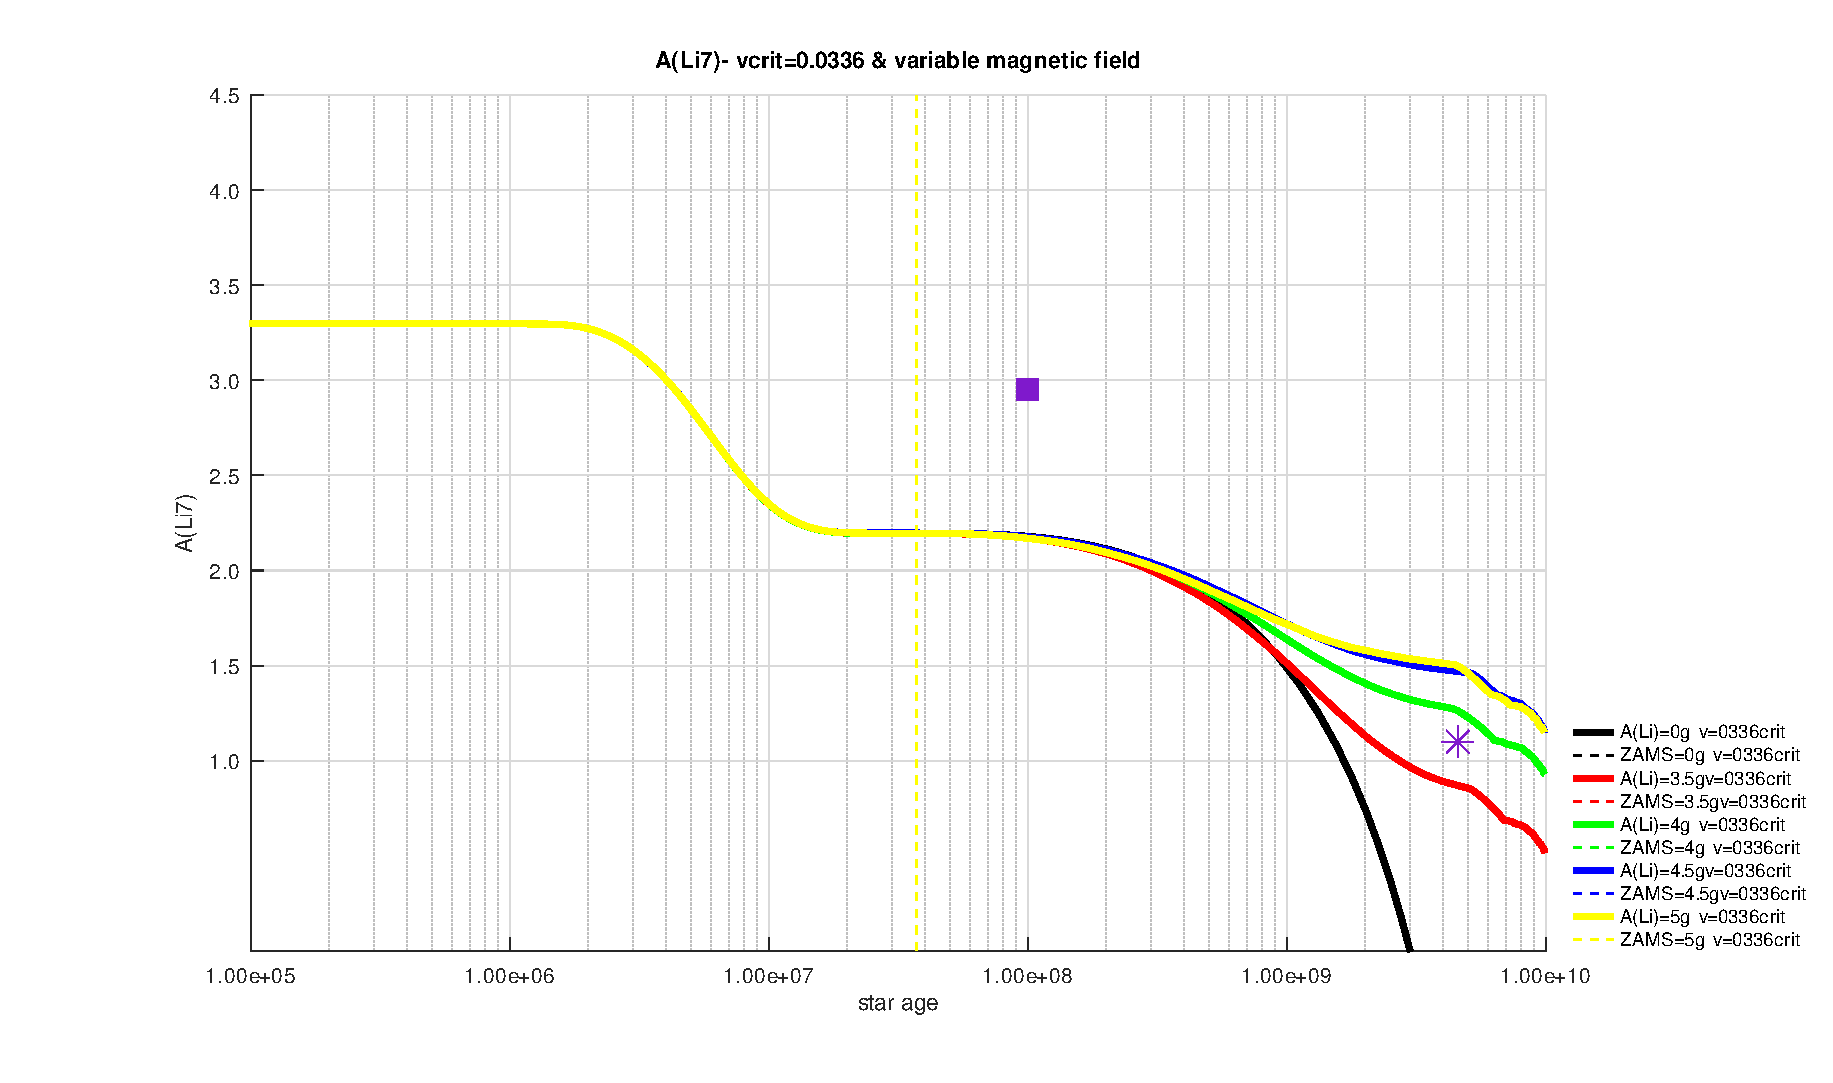
\includegraphics[width=\textwidth]{figures/li_vc_0336_var_b.eps}
    \label{fig:subim25}
    \end{subfigure}
    \begin{subfigure}[h]{0.47\textwidth}
    \includegraphics[width=\textwidth]{figures/blank.eps}
    \label{fig:subim26}
    \end{subfigure}
\caption{The evolution of surface rotational velocity, as a function of time for several 1 $M_{\sun}$ models. The lines are models with includes PMS rotation with $v/v_{crit}$ between 0.0084 and 0.0336, respectively. The purple star is the surface Li abundance for the present-day Sun \citep{Asplund2009}. The dashed lines make reference to the ZAMS defined as the temporal simulation instant closest to the timestep in which both the central H mass fraction has been reduced by 0.0015 from its initial value and the model first $L_H/L_{phot} \geq 0.99$, where $L_{H}$ is luminosity produced by the H burning power at the star core and $L_{phot}$ represents the star luminosity in the photosphere.}
\label{fig:image22}
\end{figure*}


\begin{figure*}
    \centering
    \begin{subfigure}[h]{0.47\textwidth}
    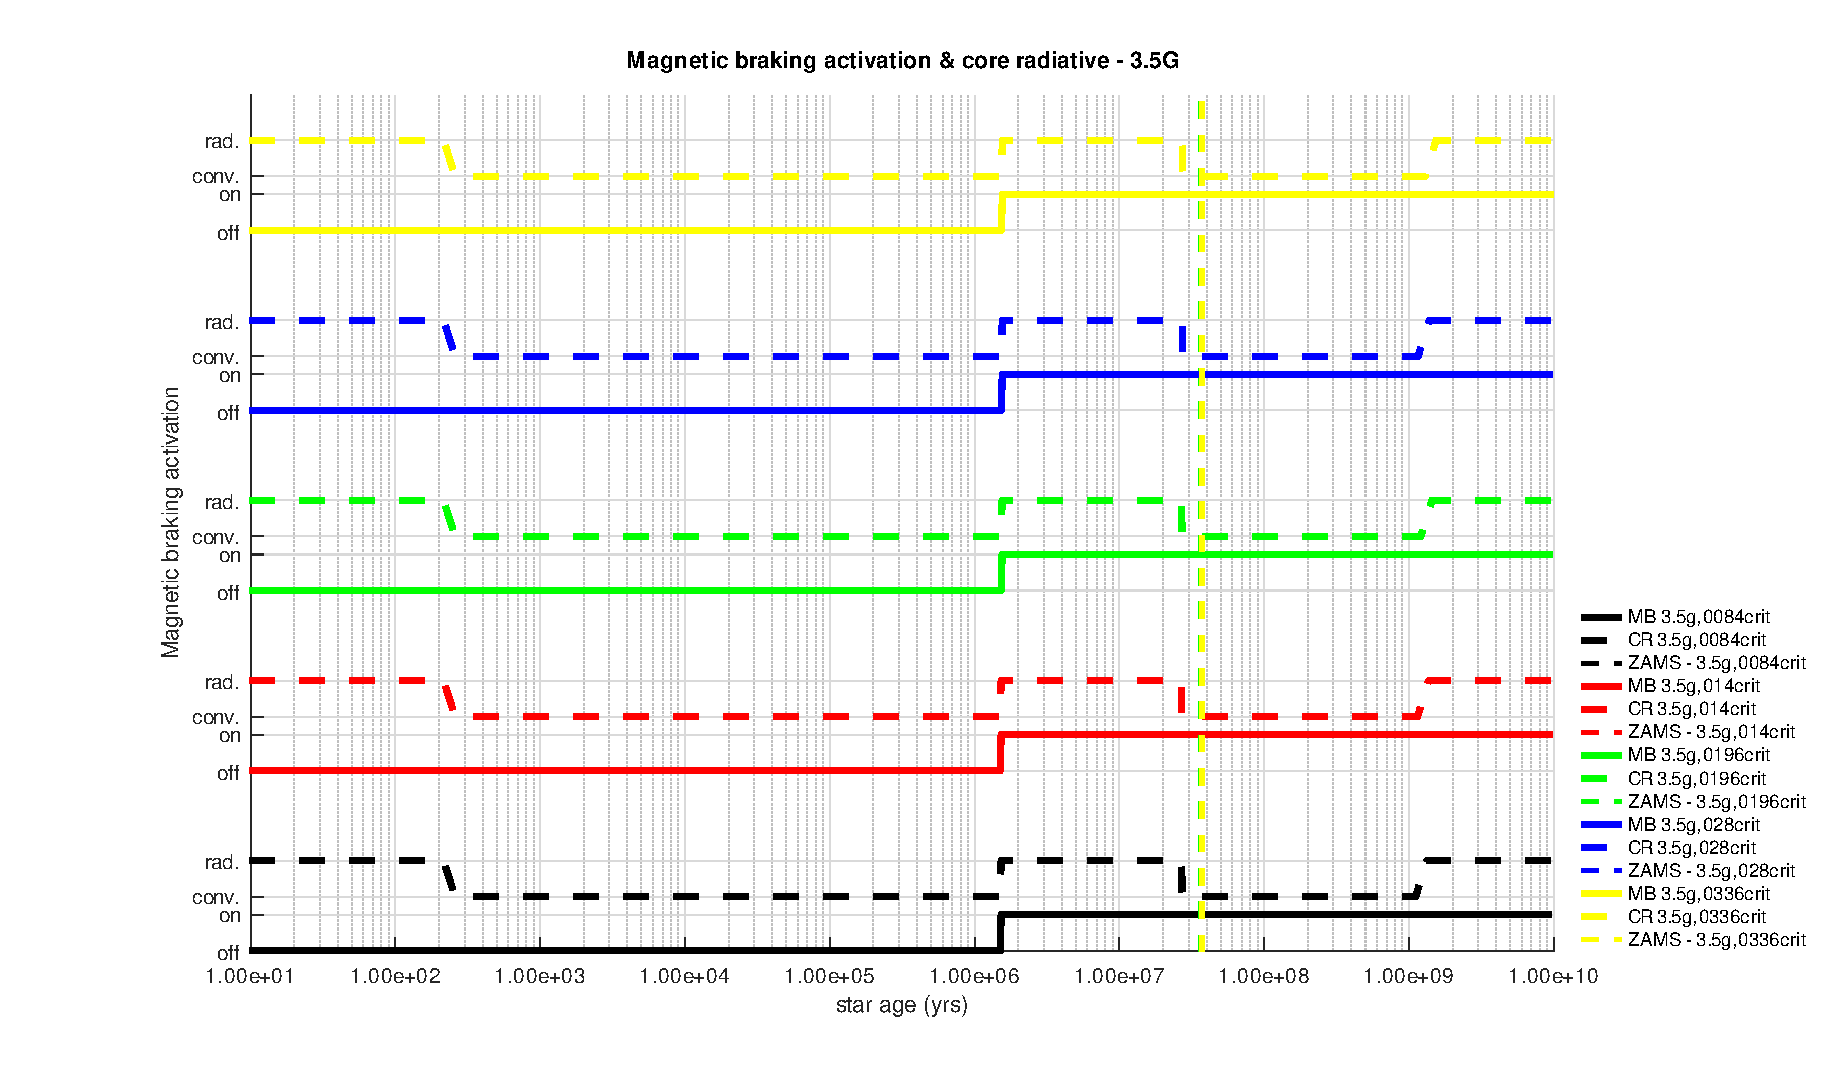
\includegraphics[width=\textwidth]{figures/mb_act_3_5g.eps}
    \label{fig:subim31}
    \end{subfigure}
    \begin{subfigure}[h]{0.47\textwidth}
    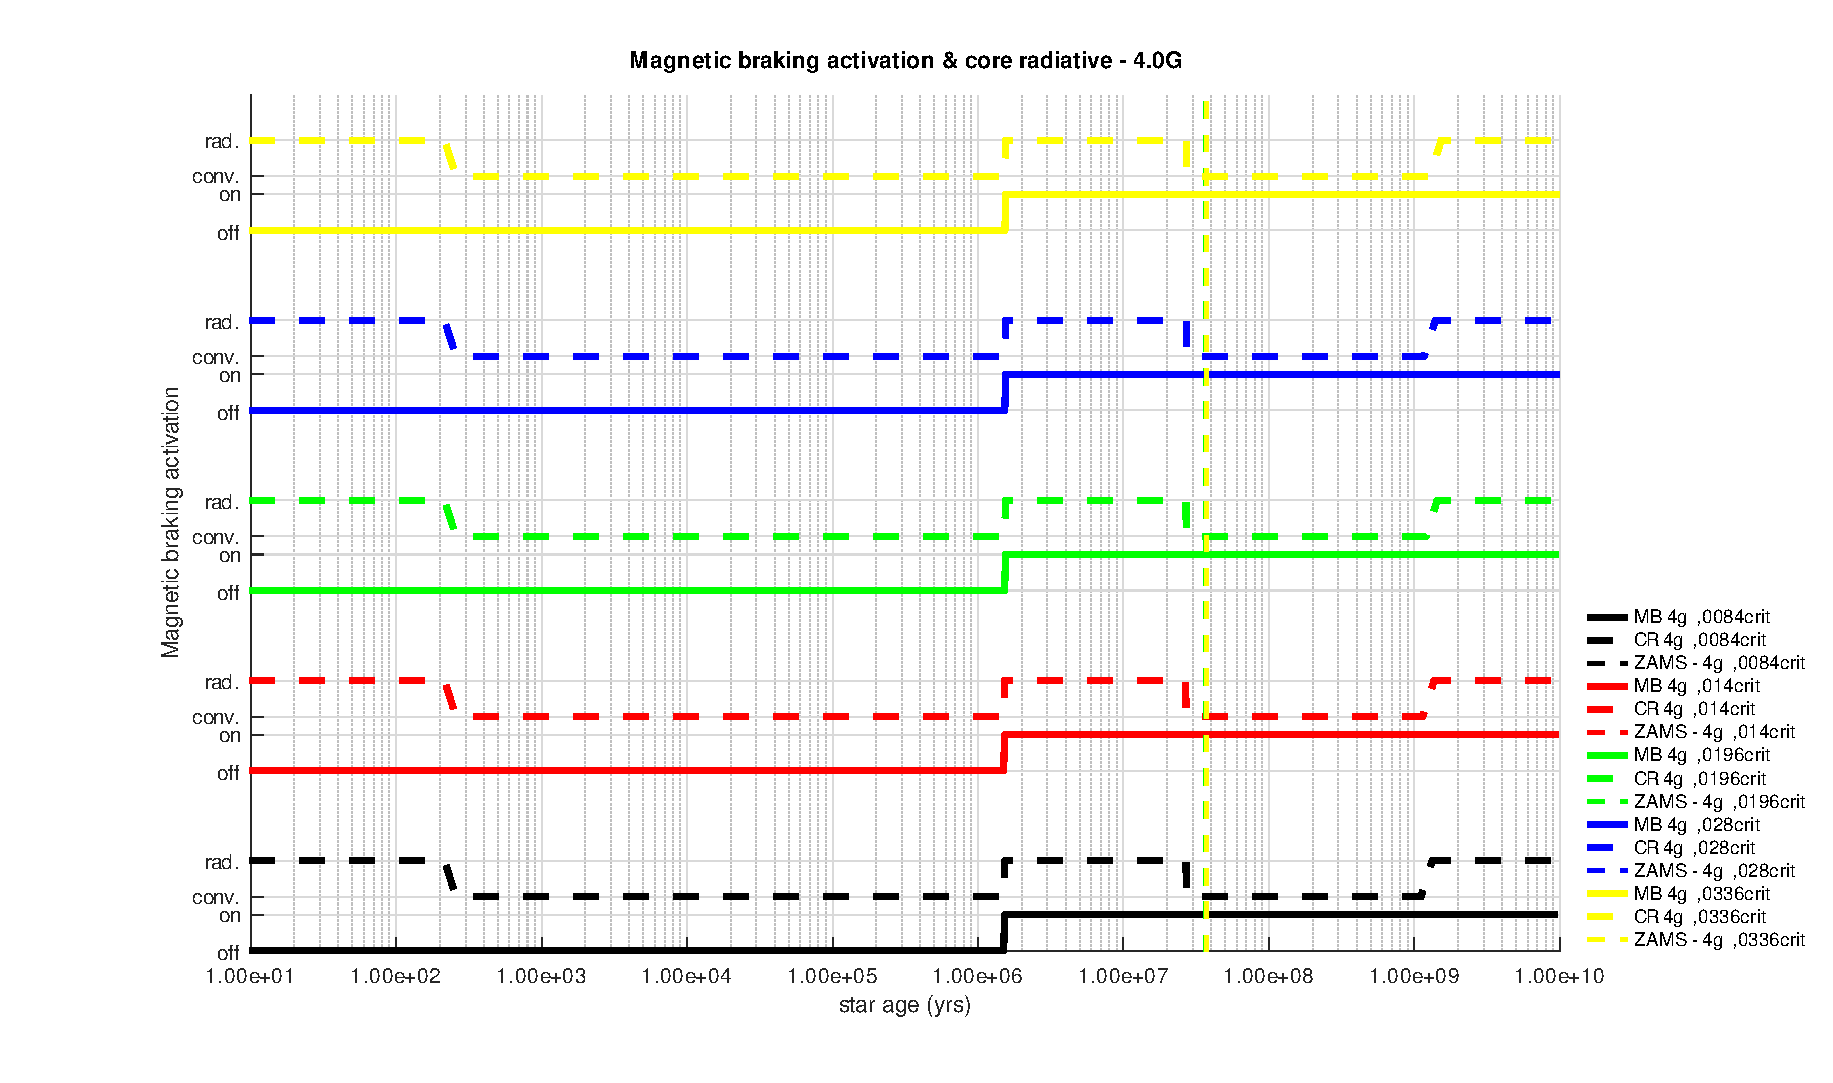
\includegraphics[width=\textwidth]{figures/mb_act_4_0g.eps}
    \label{fig:subim32}
    \end{subfigure}
    \begin{subfigure}[h]{0.47\textwidth}
    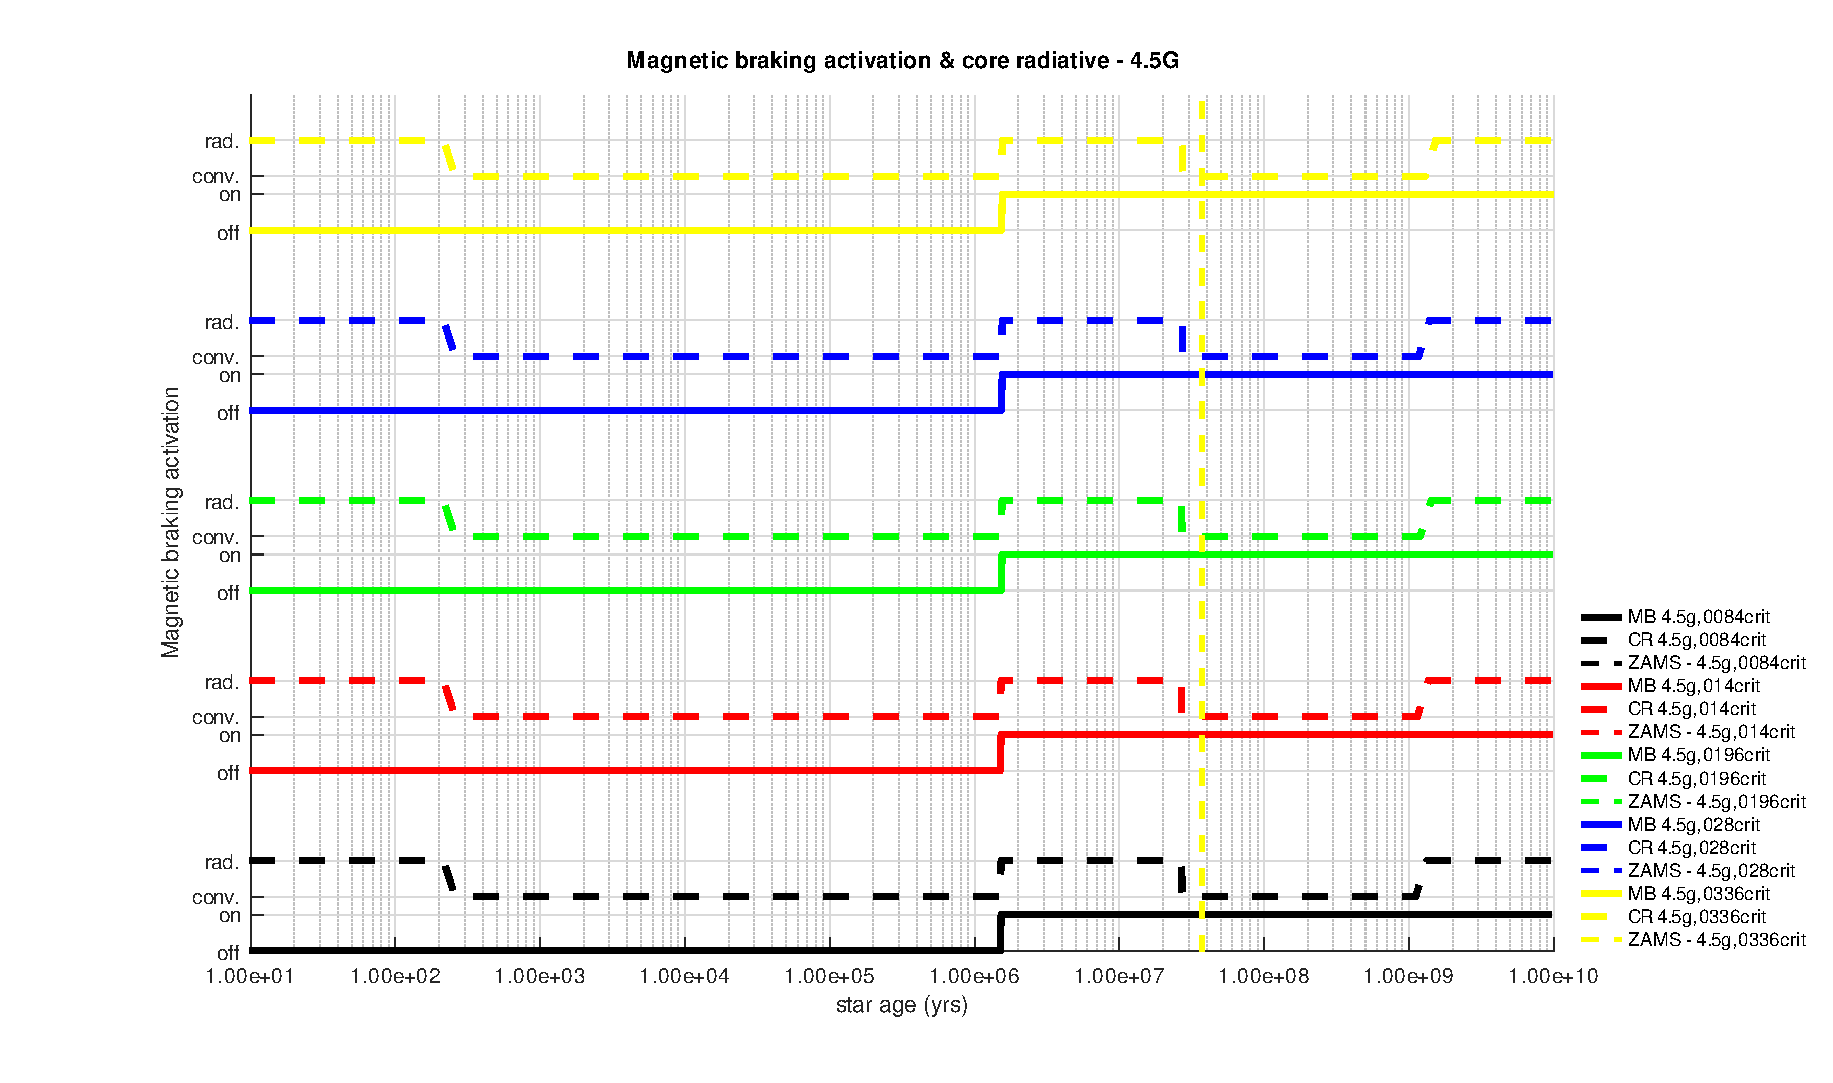
\includegraphics[width=\textwidth]{figures/mb_act_4_5g.eps}
    \label{fig:subim33}
    \end{subfigure}
    \begin{subfigure}[h]{0.47\textwidth}
    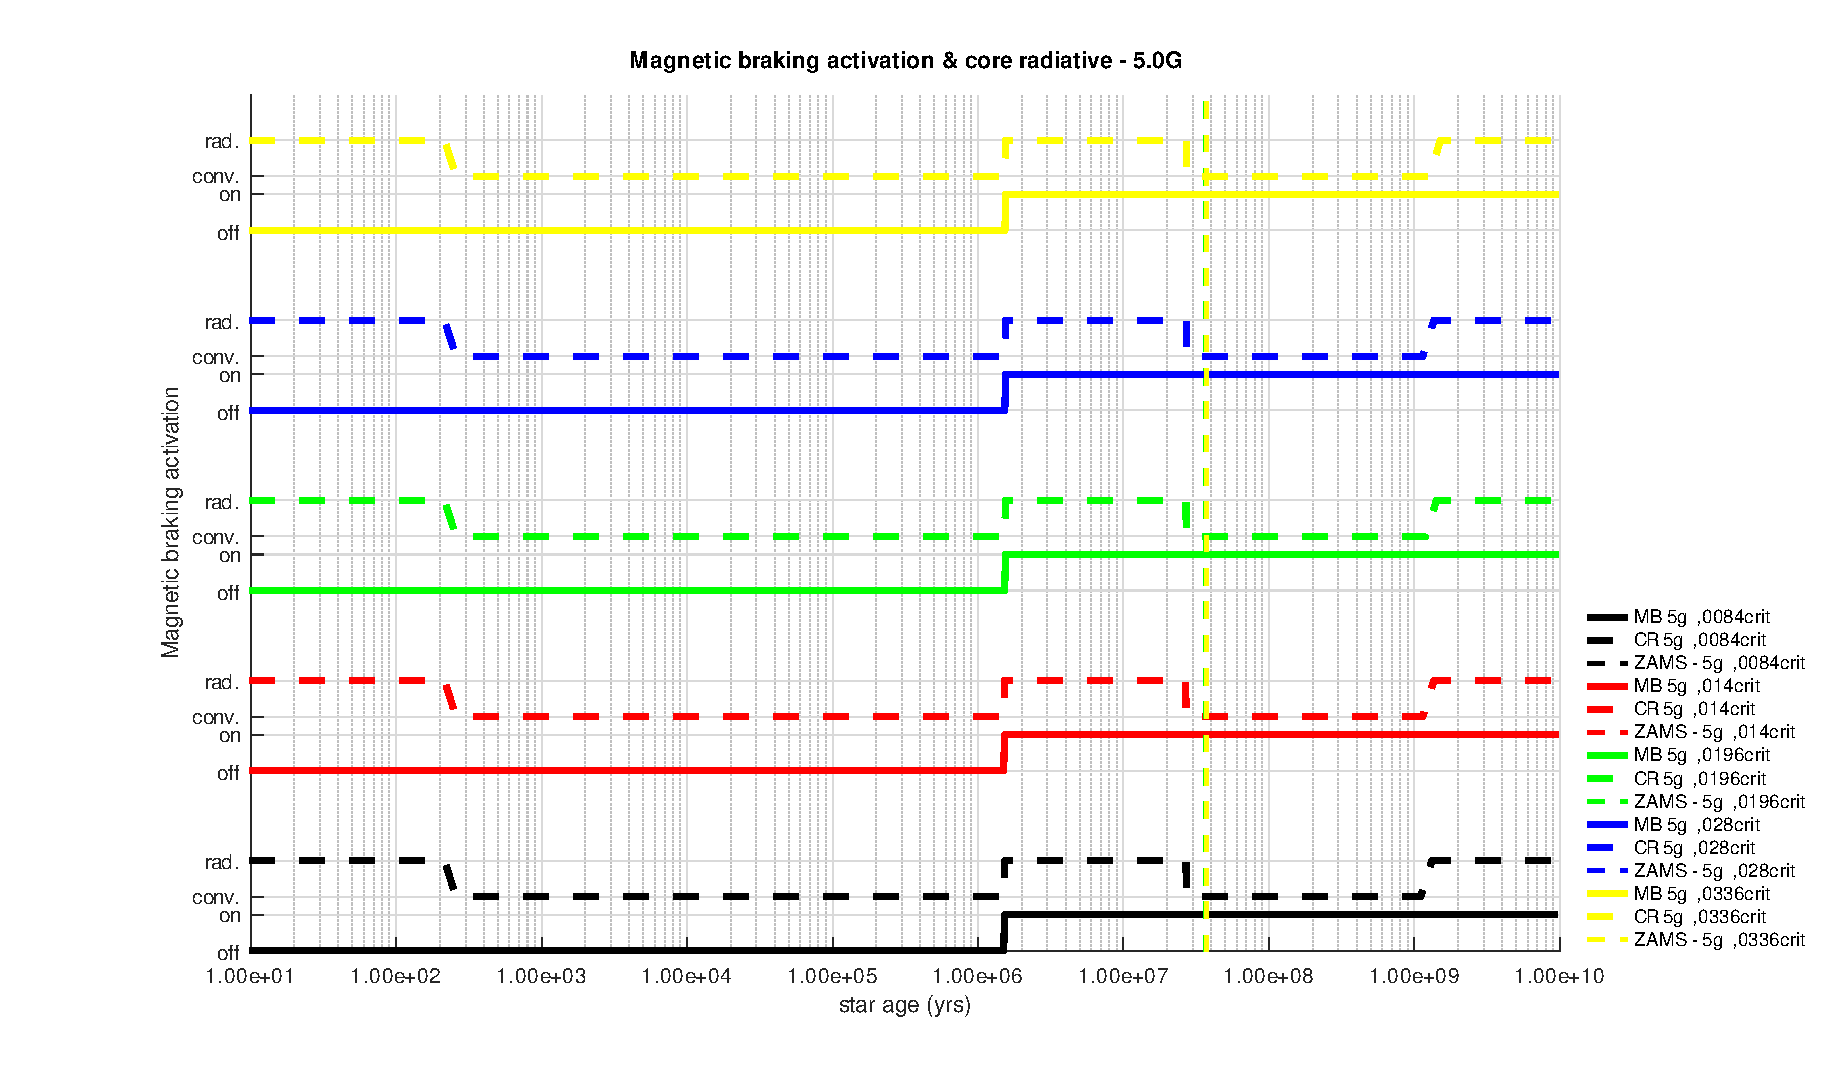
\includegraphics[width=\textwidth]{figures/mb_act_5_0g.eps}
    \label{fig:subim34}
    \end{subfigure}
    \begin{subfigure}[h]{0.47\textwidth}
    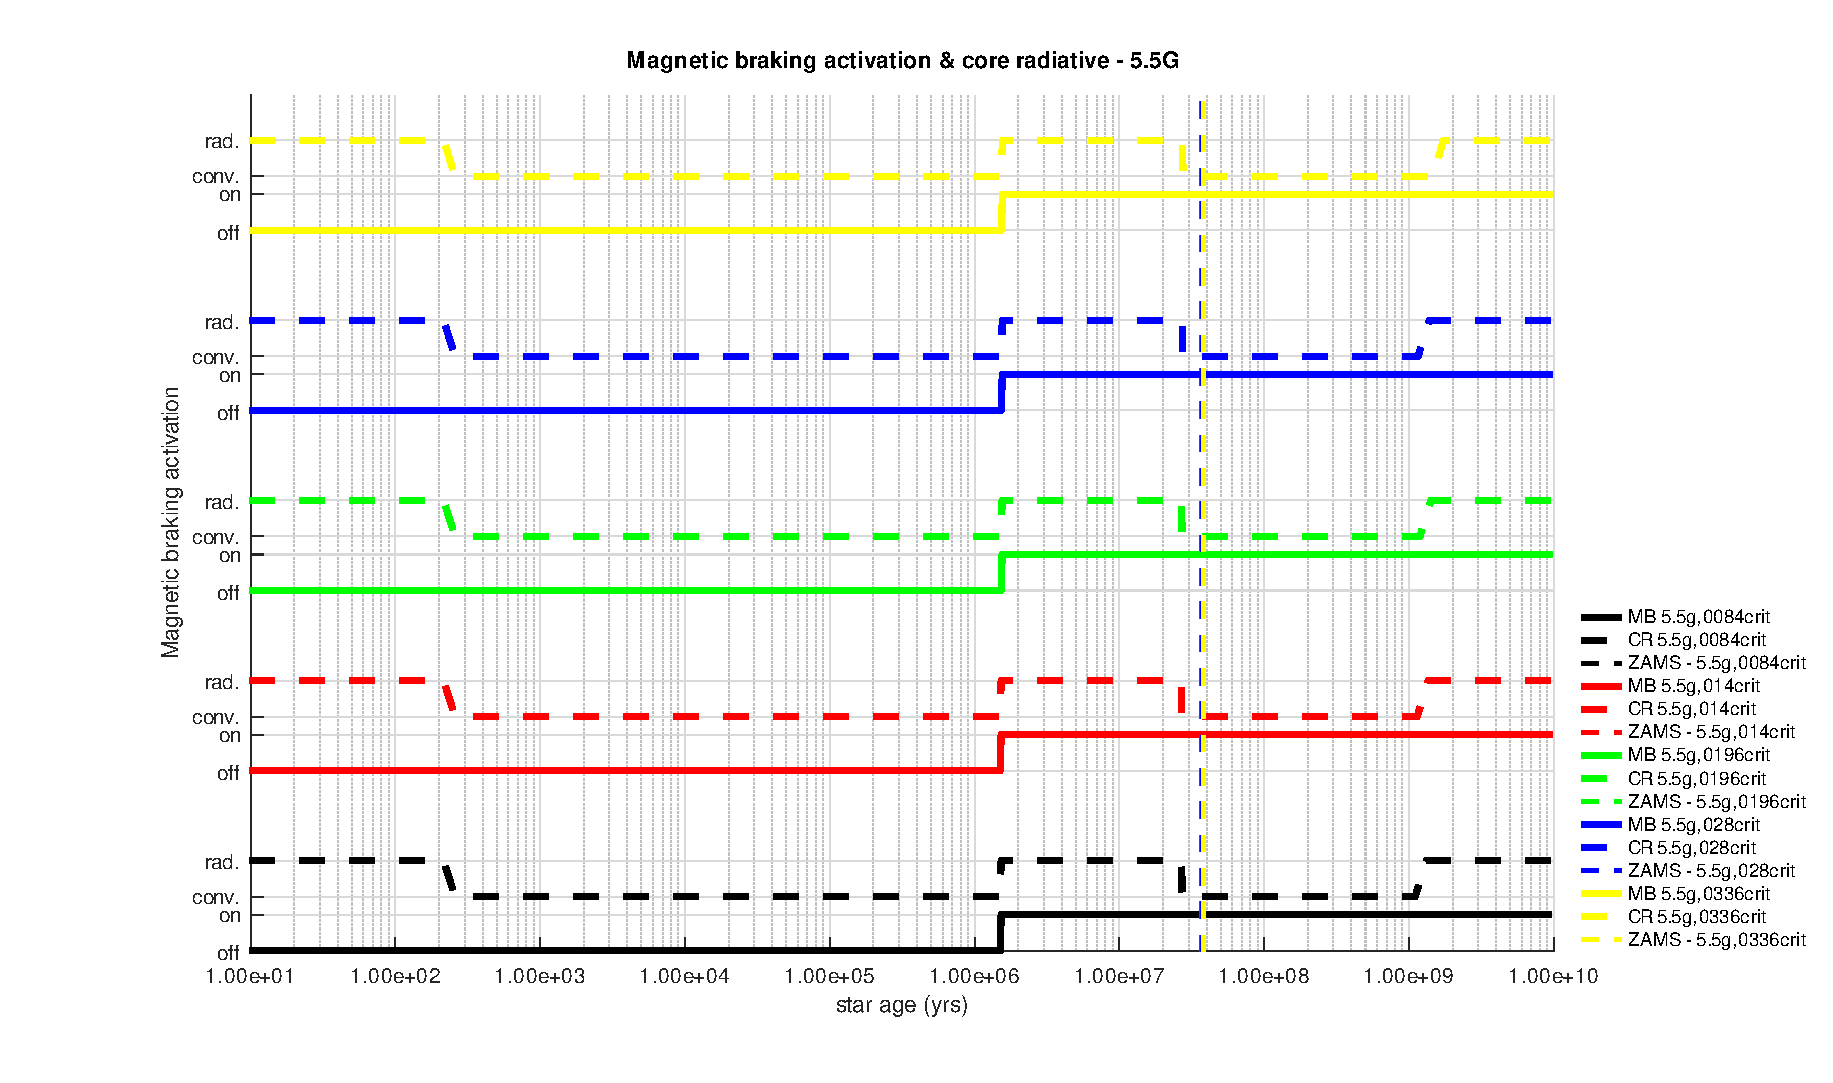
\includegraphics[width=\textwidth]{figures/mb_act_5_5g.eps}
    \label{fig:subim35}
    \end{subfigure}
    \begin{subfigure}[h]{0.47\textwidth}
    \includegraphics[width=\textwidth]{figures/blank.eps}
    \label{fig:subim36}
    \end{subfigure}
\caption{The evolution of magnetic braking activation, as a function of time and the existence of a radiative core for several 1 $M_{\sun}$ models. The lines are models with includes PMS rotation with $v/v_{crit}$ between 0.0084 and 0.0336, respectively. The dashed lines make reference to the ZAMS defined as the temporal simulation instant closest to the timestep in which both the central H mass fraction has been reduced by 0.0015 from its initial value and the model first $L_H/L_{phot} \geq 0.99$, where $L_{H}$ is luminosity produced by the H burning power at the star core and $L_{phot}$ represents the star luminosity in the photosphere.}
\label{fig:image32}
\end{figure*}



\begin{figure}
	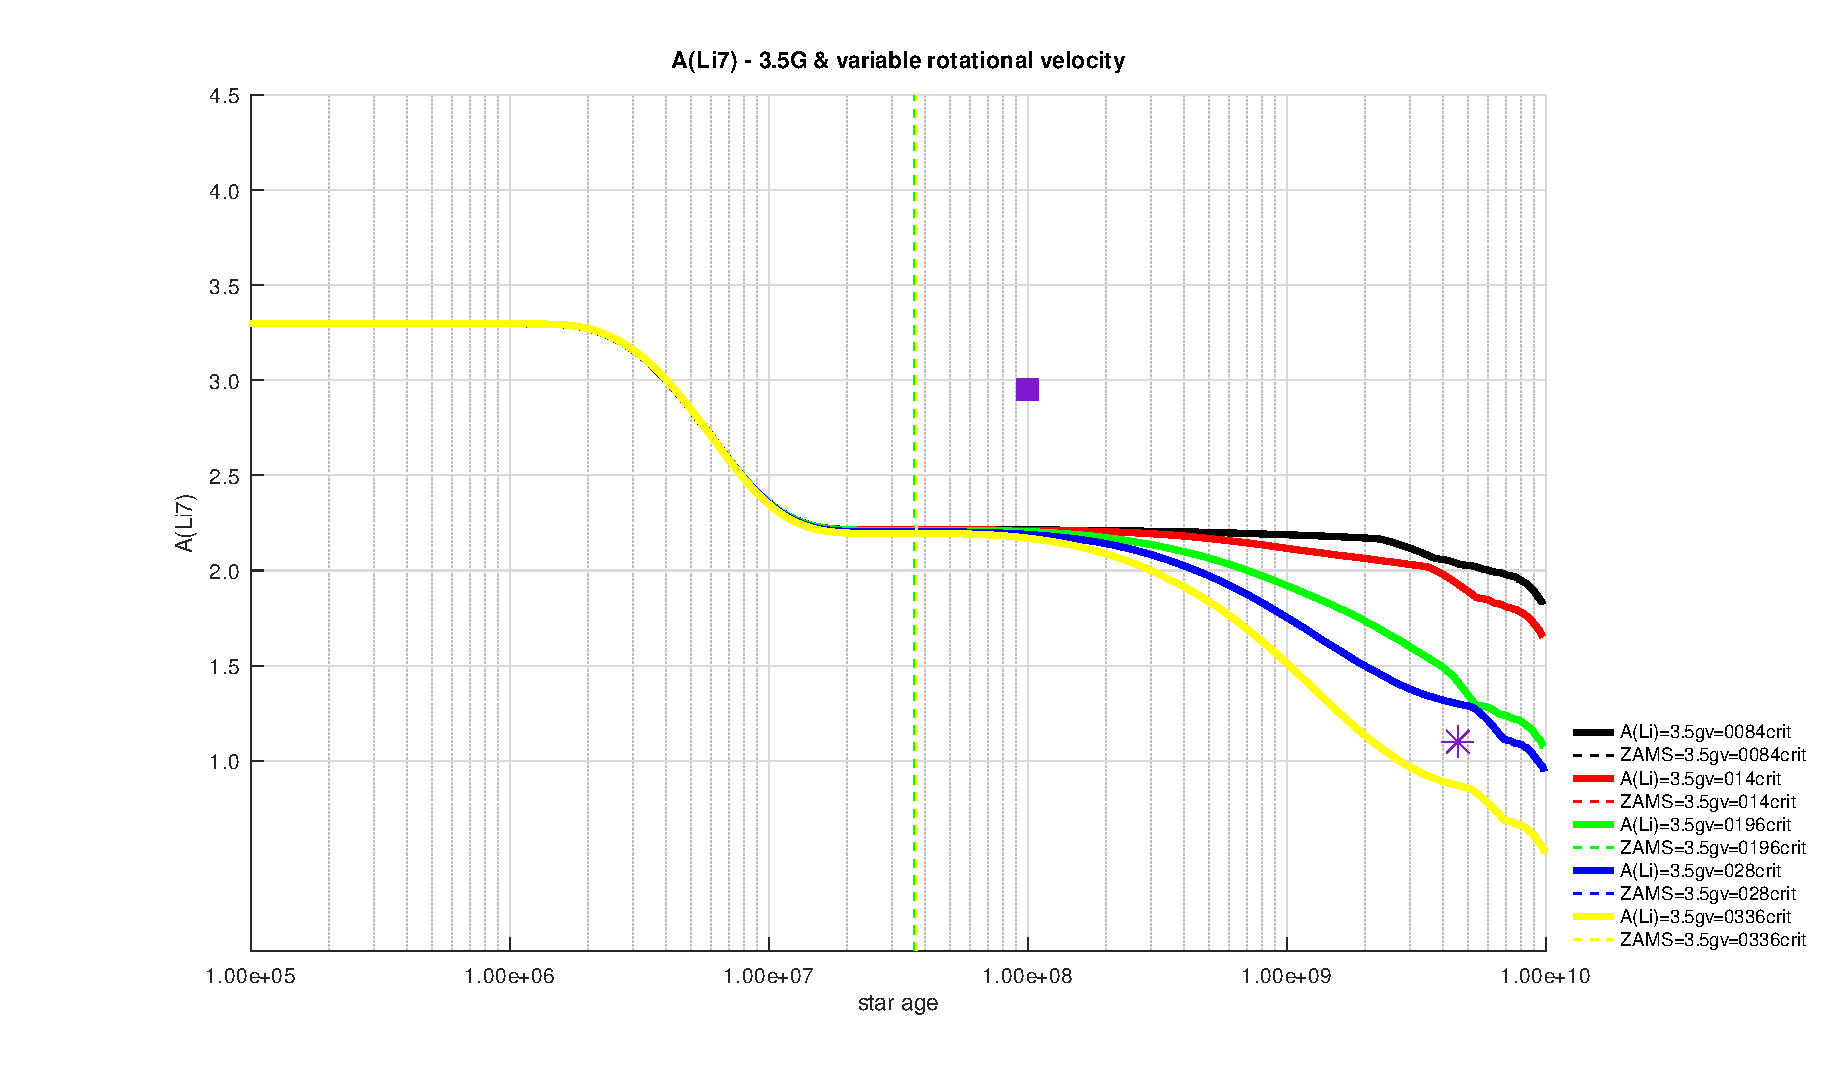
\includegraphics[width=\columnwidth]{figures/li_var_vel_3_5g.eps}
    \caption{The evolution of surface rotational velocity, as a function of time for several 1 $M_{\sun}$ models. The lines are models with includes PMS rotation with $v/v_{crit}$ between 0.0084 and 0.0336, respectively. The purple star is the surface Li abundance for the present-day Sun \citep{Asplund2009}. The dashed lines make reference to the ZAMS defined as the temporal simulation instant closest to the timestep in which both the central H mass fraction has been reduced by 0.0015 from its initial value and the model first $L_H/L_{phot} \geq 0.99$, where $L_{H}$ is luminosity produced by the H burning power at the star core and $L_{phot}$ represents the star luminosity in the photosphere.}
    \label{fig:li_var_vel_3_5g}
\end{figure}



In Figs. 2 and 3, we notice several interesting new facts for models with a magnetic field:
- the models have almost an internal solid body rotation, with a difference of only a few percent between the core and the bulk of the envelope, with a short transition at their inter- face. The differential rotation parameter q is very small, but still different from zero. The relative constancy of $\Omega$ is the result of the high value of the transport coefficient ν by the magnetic field (see below Fig. 8). We notice that these results are in agreement with those of Heger et al. (2004), who also find essentially solid body rotation until the end of the MS phase. Then in later phases, differential rotation appears together with a slowing down of the core;
- there is a general slowing down of rotation during evolution due to two effects: the mass loss which removes angular momentum and the expansion of the external layers. The strong internal coupling of rotation transports this slowing down to the core;
- models M 1 and M 5, although not strictly identical (see Fig. 4), exhibit similar $\Omega$ distributions;
- we notice a small decrease of $\Omega$ near the surface. This is likely resulting from the expansion of the superficial layers after the removal of some mass by stellar winds at the surface.


red lines are models with less and more efficient overshoot, resulting in reduced and enhanced lithium depletion, respectively. The three dot-dashed lines show additional variations in input
physics: the red lines correspond to a MLT = 1.7 , while the orange and green lines are models that include PMS rotation with v v crit = 0.01 and 0.10, respectively. As expected, a lower a MLT produces a puffier, cooler star, resulting in less lithium depletion. The inclusion of rotation during the PMS produces very different, potentially more promising behavior, though the current absence of magnetic braking (see Sec-
tions 3.6.5 and 3.5) in MESA results in an unrealistically high rotation speed ( v v crit between 0.1 and 1) on the MS. The models presented here fail to simultaneously match both the young and present-day solar surface lithium abundances.





\section{Conclusions}
The inclusion of rotation during the PMS and magnetic braking during MS produces very different, potentially more promising behavio, though magnetic braking during PMS seems to be also required for explaining Li abundances in young clusters.

The Teff’s from standard evolutionary tracks represent upper limits since these models do not include the magnetic field effect on the thermal structure.
Inclusion of the magnetic field leads to cooler models and lower Li depletions in the PMS. 

¿Para la cabecera?
This generally neglected physical input ( thermal modifications that are due to the magnetic field) affects the location of the PMS: tracks that do not allow for the effect of the magnetic field on the convective Teff gradients provide an upper limit to the.
This new feature in MESA is not equivalent to an artificial parametric change of the convection efficiency.
We also point out that more complete models are needed, including a self-consistency model between the dynamo
magnetic field and the evolution of stellar rotation.

Mass loss by stellar winds drastically reduces vrot during the evolution (Packet
et al 1980; Langer \& Heger 1998; Figs. 3 and 4). Even if isotropic, the stellar winds carry away quite a lot of angular momentum, and this is even more important in the case of equatorial mass loss. The new surface layers then have a lower vrot as a result of expansion and redistribution.



Indicar que se hace un planteamiento relativamente sencillo para la existencia de un campo magnético: existencia de núcleo radiativo y envelope convectivo. Para un tratamiento más avanzado se puede recurrir al documento (pag 10) "Stellar Evolution with rotation and magnetic fields" (Maeder \& Meynet)

Página 6 de "On the revolution ofrotational velocity..." hay un planteamiento teórico para hacer dependiente la intensidad del campo magnético. Utilizar esto para futuros planteamientos. En la página 16 deriva la fórmula para el cálculo de la pérdida de momento angular. Utilizarla para enlazar con la versión simplificada ofrecida por Cantiello.



The last numbered section should briefly summarise what has been done, and describe
the final conclusions which the authors draw from their work.

A T Tauri star is a type of pre–main sequence star that is being heated through gravitational contraction and has not yet begun to burn hydrogen at its core. They are variable stars that are magnetically active. The magnetic field of these stars is thought to interact with its strong stellar wind, transferring angular momentum to the surrounding protoplanetary disk. This allows the star to brake its rotation rate as it collapses. PODRÍAMOS INDICAR QUE YA QUE NO ACTIVAMOS EL FRENADO MAGNÉTICO DURANTE ESTA FASE SERÍA FACTIBLE QUE LA CONCENTRACIÓN DE LI FUERA SUPERIOR A LA QUE TENEMOS EN EL MODELO, ACORDE CON PLEIADES, Y QUE EL FRENADO MAGNÉTICO DURANTE LA FASE T-TAURI PERMITIESE QUE SE LLEGASE A ESE VALOR Y LUEGO FUERA REDUCIENDO LA VELOCIDAD PARA QUE NO TERMINARA DESTRUYENDO MÁS DE LA CUENTA.

\section*{Acknowledgements}

The Acknowledgements section is not numbered. Here you can thank helpful
colleagues, acknowledge funding agencies, telescopes and facilities used etc.
Try to keep it short. xxxx

%%%%%%%%%%%%%%%%%%%%%%%%%%%%%%%%%%%%%%%%%%%%%%%%%%

%%%%%%%%%%%%%%%%%%%% REFERENCES %%%%%%%%%%%%%%%%%%

% The best way to enter references is to use BibTeX:

\bibliographystyle{mnras}
%\bibliography{magbrlitium} % if your bibtex file is called example.bib
\bibliography{mblithium}


% Alternatively you could enter them by hand, like this:
% This method is tedious and prone to error if you have lots of references
%\begin{thebibliography}{99}
%\bibitem[\protect\citeauthoryear{Author}{2012}]{Author2012}
%Author A.~N., 2013, Journal of Improbable Astronomy, 1, 1
%\bibitem[\protect\citeauthoryear{Others}{2013}]{Others2013}
%Others S., 2012, Journal of Interesting Stuff, 17, 198
%\end{thebibliography}

%%%%%%%%%%%%%%%%%%%%%%%%%%%%%%%%%%%%%%%%%%%%%%%%%%

%%%%%%%%%%%%%%%%% APPENDICES %%%%%%%%%%%%%%%%%%%%%

\appendix

\section{Some extra material}

If you want to present additional material which would interrupt the flow of the main paper,
it can be placed in an Appendix which appears after the list of references.

%%%%%%%%%%%%%%%%%%%%%%%%%%%%%%%%%%%%%%%%%%%%%%%%%%


% Don't change these lines
\bsp	% typesetting comment
\label{lastpage}
\end{document}

% End of mnras_template.tex